%%%%%%%%%%%%%%%%%%%%%%%%%%%%%%%%%%%%%%%%%%%%%%%%%%%%%%%%%%%%%%%%%%%%%%%%%%%
% filename    : sp.tex
% author      : Johcel Gene T. Bitara & Miguel Damien L. Garcera
%%%%%%%%%%%%%%%%%%%%%%%%%%%%%%%%%%%%%%%%%%%%%%%%%%%%%%%%%%%%%%%%%%%%%%%%%%%

% BUGFIX: Save LaTeX kernel version of \@xfloat
\makeatletter
\let\my@xfloat\@xfloat
\makeatother

% use ateneo de naga etd class (actually modified virginia tech's etd class)
\documentclass[oneside]{etd}

% BUGFIX: Create a modified copy of \@xfloat using the kernel definition
\makeatletter
\def\@xfloat#1[#2]{
	\my@xfloat#1[#2]%
	\def\baselinestretch{1}%
	\@normalsize \normalsize
}
\makeatother

% use these packages

\usepackage{graphicx}
\usepackage{amssymb}
\usepackage{gensymb}
\usepackage{latexsym}
\usepackage{amsmath}
\usepackage{booktabs}
\usepackage{multirow}
\usepackage{pifont}
%\usepackage[lineno5,noindent]{lgrind}
%\usepackage{rotating} 
%\usepackage{makeidx}
%\usepackage{stmaryrd}
\usepackage{float}
\usepackage{subfigure}
%\usepackage{cite}
%\usepackage{moreverb}
%\usepackage{pictexwd,dcpic}
\usepackage{algorithm,algorithmic}
\renewcommand{\algorithmicrequire}{\textbf{Input:}}
\renewcommand{\algorithmicensure}{\textbf{Output:}}
\usepackage{tikz}
\usetikzlibrary{positioning,calc}
\usepackage[T1]{fontenc}
\usepackage{xparse}
\usepackage{enumitem}
\usepackage{parskip}
\setlist[description]{
  labelsep=0pt,
  labelwidth=\transcriptlen,
  leftmargin=\transcriptlen,
}

\newlength{\transcriptlen}

\NewDocumentCommand {\setspeaker} { mo } {%
  \IfNoValueTF{#2}
  {\expandafter\newcommand\csname#1\endcsname{\item[#1:]}}%
  {\expandafter\newcommand\csname#1\endcsname{\item[#2:]}}%
  \IfNoValueTF{#2}
  {\settowidth{\transcriptlen}{#1}}%
  {\settowidth{\transcriptlen}{#2}}%
}

\usepackage{listings}
\definecolor{cppred}{rgb}{0.6,0,0} % for strings
\definecolor{cppgreen}{rgb}{0.25,0.5,0.35} % comments
\definecolor{cpppurple}{rgb}{0.5,0,0.35} % keywords
\definecolor{cppdocblue}{rgb}{0.25,0.35,0.75} % doc
 
\lstset{
  basicstyle=\linespread{0.8}\ttfamily\small,
  keywordstyle=\color{cpppurple}\bfseries,
  stringstyle=\color{cppred},
  commentstyle=\color{cppgreen},
  morecomment=[s][\color{cppdocblue}]{/**}{*/},
  numbers=left,
  numberstyle=\tiny\color{black},
  % stepnumber=2,
  numbersep=10pt,
  tabsize=4,
  showspaces=false,
  showstringspaces=false
}

\graphicspath{{figures/}{./}}

%\renewcommand{\floatpagefraction}{0.8}

\makeindex

%%%%%%%%%%%%%%%%%%%%%%%%%%%%%%%%%%%%%%%%%%%%%%%%%%%%%%%%%%%%%%%%%%%%%%%%%%%

\title{Redesigning ADNU-HR Information System: Migrating Internal Processes Through a Customized Strategic Web Application.}
\department{Computer Science}
\BSproject % options: \BSthesis \BSproject \BShonors \Mdegree \MSdegree \PhDdegree
\degreemonth{16 July}  % date of final defense
\degreeyear{2024}

\twostudents % options: \onestudent \twostudents \threestudents \fourstudents
{Johcel Gene T. Bitara}
{Miguel Damien L. Garcera}

\studentsheader
{Bitara, Garcera}

\twodegrees % options: \onedegree \twodegrees \threesdegrees \fourdegrees
{Information Technology}
{Information Technology}

\advisor
{Joshua C. Martinez, MIT}
\threemembers
{Estrella H. Montealegre}
{Adrian Leo T. Pajarillo, MS}
{Raphael Henry M. Garay}
\deanandchair
{Joshua C. Martinez, MIT}
{Lowie Vincent Bisana, MIT}

\keywords{Human Resources Management, Information Systems, Systems Migration}

\begin{document}

%edit etd.cls to accommodate lesser number of proponents
\maketitle
\makerecomm
\makeacceptance
\makedeclaration

%%%%%%%%%%%%%%%%%%%%%%%%%%%%%%%%%%%%%%%%%%%%%%%%%%%%%%%%%%%%%%%%%%%%%%%%%%%
%                    ABSTRACT/EXECUTIVE SUMMARY                           %
%%%%%%%%%%%%%%%%%%%%%%%%%%%%%%%%%%%%%%%%%%%%%%%%%%%%%%%%%%%%%%%%%%%%%%%%%%%

% can use execsummary or abstract
\begin{abstract}
    One of the main challenges of the Ateneo De Naga University is the major limitation of the current Human Resource (HR) legacy system hindering efficient and streamlined HR processes. To resolve this is to propose a new redesign and implementation of a new Human Resources Information System (HRIS) at Ateneo de Naga University to address the limitations of the current legacy system. The study aims to centralize and standardize personal information management across departments, ensuring data integrity and efficiency in HR processes. The project involves a thorough analysis of the current HRIS, identifying unique cases different from other systems, designing a modernized application with standardized data elements, and executing a robust data migration strategy with the University's Integrated Information System (UIIS). The significance of this study lies in improving personnel information management, increasing efficiency in branch administration, and promoting centralized authority and standardized procedures. With this new HRIS, operational workflow is streamlined for HR personnel, employees, and administrators, enhancing transparency, and efficiency with HR records, and maintaining accurate, complete, and reliable data by reducing errors of inconsistencies and data redundancies ensuring integrity.
\end{abstract}

\begin{dedication}

We dedicate this research work to all of humanity.

\end{dedication}


\begin{acknowledgements}

The team extends their sincerest gratitude to all of those who have contributed to the completion of this capstone project.
\\

We would like to give our thanks and gratitude to our adviser, Mr. Joshua C. Martinez, MIT, for his invaluable guidance and support towards the project and throughout the duration of this study. 
\\

We would like to also give our thanks to Ms. Estrella H. Montealegre, Management Information System (MIS) Director, for her invaluable guidance, acknowledgment, and support for the approval of the project to become an MIS migration initiative. Without her approval, this project would not have been possible in the first place. 
\\

We are also grateful to the faculty members of the Department of Computer Science for their assistance, comments/suggestions, and advice to the team.
\\

Finally, we extend our gratitude to the staff and administrators of Ateneo de Naga University's Human Resource employees for their cooperation and assistance in providing access to resources and information necessary for this study. Their assistance made this project more concrete and achievable.
\\

\end{acknowledgements}


\begingroup
\renewcommand*{\addvspace}[1]{}
\tableofcontents
\listoffigures
\listoftables
\endgroup

\beginbody
\pagenumbering{arabic}

%%%%%%%%%%%%%%%%%%%%%%%%%%%%%%%%%%%%%%%%%%%%%%%%%%%%%%%%%%%%%%%%%%%%%%%%%%%
\chapter{Introduction}
%%%%%%%%%%%%%%%%%%%%%%%%%%%%%%%%%%%%%%%%%%%%%%%%%%%%%%%%%%%%%%%%%%%%%%%%%%%
Human Resource Management (HRM) plays an important role in the success and efficiency of institutions. HRM is responsible for managing the most valuable asset of any organization—its people. The primary functions of HRM include recruitment, training, development, performance management, and employee relations. These functions are essential for building a productive and thriving workforce, which is crucial for achieving organizational goals and maintaining a competitive edge in the market \cite{a12019,t12020}.

HR professionals act as strategic partners to the management team, advising on managing human resources effectively to meet the institution's current and future needs. They are involved in developing strategies for talent acquisition, employee retention, and skill development, ensuring the workforce is aligned with the organization's objectives. Additionally, HRM plays a significant role in fostering a positive work environment, enhancing employee engagement, and building loyalty and commitment among employees \cite{b12021,d12022}.

A Human Resources Information System (HRIS) is a software solution designed to manage and automate core HR processes. HRIS serves as a centralized repository for employee data, facilitating efficient data management, payroll processing, benefits administration, time and attendance tracking, and performance management \cite{m22024,o12023}. The implementation of an HRIS transforms HR from an administrative function to a strategic one, enabling HR professionals to focus on more value-added activities such as strategic planning and decision-making \cite{n12023}.

By automating routine HR tasks, HRIS reduces the administrative burden on HR professionals, allowing them to allocate more time to strategic initiatives. This automation leads to increased efficiency, accuracy, and compliance with labor laws and regulations. Moreover, HRIS provides real-time data access and advanced analytics capabilities, which are essential for informed decision-making and strategic workforce planning \cite{gym12024,h12022}.

HRIS also enhances the employee experience by offering self-service portals where employees can access and update their personal information, request time off, and manage their benefits. This not only improves employee satisfaction but also reduces the workload on HR staff. Furthermore, the integration of HRIS with other business systems ensures seamless data flow and consistency across the organization, contributing to overall operational efficiency \cite{a22023,s12022}.

\section{Project Context}
    
    The Human Resource and Management Office (HRMO) at Ateneo de Naga University has been utilizing a system that has served the institution well over the years. This system, consisting of disparate databases and applications, has been instrumental in managing HR processes and maintaining employee records. However, as the university has grown, the limitations of this system have become more apparent. The separation of the HRIS schema from the University Integrated Information Systems (UIIS) has led to challenges such as data duplication and the need for more streamlined processes. These issues can hinder the effectiveness of HR operations, making it difficult to manage the increasing volume of data and integrate with other university systems.
    
    To address these challenges and support the university's continued growth, there is a need to develop and implement a centralized HRIS. This new system will ensure data consistency, accuracy, and accessibility, thereby streamlining HRMO processes and improving overall data management. The centralized HRIS will also facilitate better integration with other university systems, enhancing the institution's ability to manage HR data comprehensively and efficiently. The new HRIS will be designed to interact seamlessly with various stakeholders within the university. HRMO personnel will be responsible for data entry, managing employee records, and processing HR-related tasks. University management will access HR data for decision-making and strategic planning. Other departments requiring HR data for various administrative and operational purposes will also benefit from the new system.

    The study will involve key stakeholders who will provide valuable insights and feedback throughout the project. HRMO personnel, with their firsthand experience with the current system, will help identify areas for improvement and define requirements for the new HRIS. MIS office personnel, with their technical expertise, will be crucial in designing and implementing the new system. University management will ensure that the new HRIS aligns with the institution's overall goals and objectives. The new HRIS will handle various types of data to support HR operations. Input data will include employee records, attendance data, leave applications, and other HR-related information. Output data will consist of reports on employee information, attendance, leave status, and other HR metrics. These reports will be essential for decision-making, compliance, and strategic planning.
    
\section{Purpose and Description}

    The main purpose of the project is to redesign, develop and implement a centralized Human Resource Information System (HRIS) to enhance data management, streamline HR processes, and support the university's growth. This initiative aims to address the limitations of the current system by providing a more integrated and efficient solution that meets the evolving needs of the institution.

    The project will begin with an information-gathering and system analysis phase. This initial phase will involve collecting detailed feedback from HRMO personnel, university management, and other stakeholders to understand the current system's limitations and requirements. Analyzing the existing system will help identify specific areas that need improvement and features that should be incorporated into the new HRIS. Following the analysis, the project will proceed with the design and development of the new HRIS. This includes creating modules for attendance monitoring, leave management, user authentication, and report generation. 
    
    The new system will be designed to accommodate the current requirements that the current system was unable to fully support. Additionally, the project will focus on redesigning HR workflows to make them more efficient and user-friendly. Integration with other university systems will be a key component, ensuring seamless data flow and accessibility across different departments. Finally, the project will involve migrating existing employee data to the new HRIS, ensuring that no valuable information is lost in the transition.

    The new HRIS will bring substantial benefits to various stakeholders within the university:
    
    \begin{itemize}
        \item[] \textbf{HRMO personnel.} The new HRIS will significantly improve data integrity and streamline HR processes, allowing HRMO staff to manage employee information more effectively. This will reduce the time spent on manual data entry and corrections, enabling staff to focus on more strategic HR activities.

        \item[] \textbf{University Management.} University management will benefit from enhanced reporting and analytics capabilities provided by the new HRIS. This will facilitate better decision-making and strategic planning by providing accurate and up-to-date HR data.

        \item[] \textbf{Employees.} Employees will experience more efficient HR services, such as faster processing of leave applications and more accurate attendance tracking. The user-friendly interface of the new HRIS will also make it easier for employees to access and update their personal information.

        \item[] \textbf{Departments.} Other departments that require HR data for various administrative and operational purposes will benefit from the improved data accessibility and integration with other university systems. This will ensure that all departments have access to consistent and accurate HR information.

        \item[] \textbf{The University.} The university will benefit from a scalable system that supports future growth and integration needs. The new HRIS will facilitate easier access, management, and reporting of employee data, thereby enhancing overall operational effectiveness. By addressing the limitations of the current system, the new HRIS will provide a robust foundation for the university's HR operations, supporting its mission and strategic goals.
    \end{itemize}
    
\section{Objectives}

    The main objective of the study is to redesign and implement the core Human Resource Information System (HRIS) functionalities for the Ateneo de Naga University. In order to achieve the main objective, the following objectives must be accomplished:

    \begin{enumerate}
        \item Collect and document data requirements to ensure they align with stakeholders' needs and project goals.
        \item Create design specifications for each system component and module, including data models and interfaces.
        \item Review and confirm the proposed system design with stakeholders to ensure it meets project requirements.
        \item Develop and implement the functionality of modules based on the defined design and requirements.

        \item Gather feedback from stakeholders on the functionality and usability of all modules.
        \item Review the completed work from each iteration and demonstrate the new features to stakeholders.
        \item Assess the system's functionality, performance, and user experience.
        \item Ensure the system meets the needs and expectations of the end-users.
        \item Conclude the testing phase and prepare test reports summarizing testing activities and results.
        \item Prepare the system and infrastructure for deployment to ensure a smooth transition to production.
        \item Deploy the system to the production environment.
        \item Develop comprehensive training materials and documentation to support end-user training.
        \item Finalize detailed technical specifications documenting the system architecture, design, and implementation details.
    \end{enumerate}
    
\section{Scope and Limitation}

    The project is focused on redesigning the Human Resource Information System (HRIS) to address the limitations of the current system and to meet the evolving needs of the university. The project will primarily concentrate on HR processes such as enhancing employee information management, streamlining performance evaluations, improving training and development tracking, maintaining comprehensive health and safety records, automating administrative tasks like generating certificates of employment and employment contracts, monitoring employee status and assignments, managing academic awards and faculty ranks, and facilitating report generation. The project shall also include the migration from the current system to UIIS. This includes covering data migration of records from the previous schema to migrating to the new HR schema and transitioning from the current system's Database Management System -- MySQL to Oracle.
    
    Additionally, the system will include functionalities for managing staff attendance and work schedules, handling leave applications and leave credits, and managing faculty attendance and schedules in connection with ADNU-ONE that cover these modules for the employee-side. This ensures that the new system is robust, user-friendly, and capable of handling the university's current and future requirements. The project will begin with gathering information and analyzing the existing system to identify its limitations and areas for improvement. This analysis will inform the design and development of the new HRIS, which will include several key modules.
    
    The modules to be developed include:
    
    \begin{itemize}
        \item[] \textbf{User Authentication and Authorization Module.} This module is essential for providing secure access mechanisms to ensure that only authenticated users have appropriate permissions within the HRIS. It will utilize GBOX accounts for user authentication, which offers easy access and enhanced security, thereby improving the overall user experience. By integrating GBOX, the system ensures that users can seamlessly log in using their existing credentials, reducing the need for multiple passwords and enhancing security through centralized authentication.
        \item[] \textbf{User Privileges.} The User Privileges module will offer comprehensive administrative tools for managing users, base tables, and other system settings. This module is crucial for security purposes as it ensures that users have the appropriate access levels and permissions based on their roles within the organization. By carefully managing user privileges, the system can prevent unauthorized access to sensitive information and maintain data integrity.
        \item[] \textbf{HRIS Modules.} These modules will contains functionalities to manage HR processes such as:
        \begin{itemize}
            \item[] \textbf{Employee Information Management:}
            Storing and managing personal and professional information of employees.

            \item[] \textbf{Performance Evaluations: }
            Streamlining the process of evaluating employee performance to ensure accurate and timely assessments.

            \item[] \textbf{Training and Development Tracking: } Recording and tracking training sessions attended by employees to support their professional growth.
            
            \item[] \textbf{Health and Safety Records: } Maintaining comprehensive health records to ensure the well-being of employees and compliance with health regulations.
            
            \item[] \textbf{Administrative Tasks: } Generating certificates of employment and employment contracts to reduce administrative burden and improve accuracy.
            
            \item[] \textbf{Monitoring Employee Status and Assignments:  } Tracking status movements and job assignments of employees to ensure proper record-keeping and organizational structure.
            
            \item[] \textbf{Managing Academic Awards and Faculty Ranks: } Handling academic awards and faculty ranks to recognize and incentivize employee achievements.
        \end{itemize}
       

        \item[] \textbf{TIMESYS: Attendance Monitoring (Staff) Modules.} These modules will handle the monitoring and recording of staff attendance. They include functionalities such as capturing login and logout times, processing raw attendance data, managing work schedules, and computing overtime. By accurately tracking attendance, the system can ensure compliance with work schedules and provide reliable data for payroll and performance evaluations.
        \item[] \textbf{FACSYS: Attendance Monitoring (Faculty) Modules.} The FACSYS modules will manage the monitoring and recording of faculty attendance. This includes tracking attendance by semester and school year, managing faculty schedules, and processing attendance reports. These modules ensure that faculty attendance is accurately recorded and reported, facilitating compliance with academic schedules and workload requirements.
        \item[] \textbf{LEAVESYS: Leave Management.} This module will manage employees' leave applications and processing. It includes storing approved leave applications, tracking leave reasons and credits, and processing leave applications with leave credits reports. By automating leave management, the system can streamline the approval process, ensure accurate tracking of leave balances, and provide valuable data for decision-making.
        \item[] \textbf{Optimized Reports Generation.} The current system lacks optimization on their reports causing delays in report generation. With this, the project aims to allow users to set parameters for reports, generate report outputs in various formats such as CSV, Excel, or PDF, and export reports efficiently for faster further analysis and record-keeping. This functionality ensures that users can easily generate and access the data they need for strategic decision-making, compliance reporting, and operational analysis.
    \end{itemize}
    
    Given the wide scope of this project, the focus will be the modules mentioned, with room for scalability to accommodate additional features for the employee view in the future. The project does not include the development of new hardware infrastructure, as it will utilize existing university resources. Additionally, modules unrelated to HR processes, such as financial management or student information systems, are not within the scope of this project.
    
    By concentrating on these areas, the project aims to create a centralized HRIS that enhances data management, streamlines HR processes, and supports the university's growth. The new system will provide a scalable and integrated solution that addresses the limitations of the current system, ultimately benefiting all stakeholders involved.



%%%%%%%%%%%%%%%%%%%%%%%%%%%%%%%%%%%%%%%%%%%%%%%%%%%%%%%%%%%%%%%%%%%%%%%%%%%
% \chapter{Review of Related Systems and Literature}
%%%%%%%%%%%%%%%%%%%%%%%%%%%%%%%%%%%%%%%%%%%%%%%%%%%%%%%%%%%%%%%%%%%%%%%%%%%

% This chapter provides the relevant literature that is essential for developing a better understanding of the problem of the study and the significance of its resolutions. Additionally, existing features and/or systems that can assist in resolving this issue are identified. Researchers found it beneficial to evaluate the gaps in existing systems as it guides in determining the features that a system should have to successfully solve the problem of the study.

% ------------------------------------------------------------------ %
% ------Review of Related Literature-------------------------------- %
% ------------------------------------------------------------------ %

\section{Review of Related Literature}
    Human Resource Information Systems (HRIS) has undergone significant transformation, driven by technological advancements and evolving organizational needs. This literature review provides a foundational understanding of HRIS and its historical progression over time from basic HR processes to complex systems that support a wide range of HR-related tasks. It emphasizes how essential HRIS is to improving corporate effectiveness, simplifying HR procedures, and enabling data-driven decision-making. It also includes the current trends as well as how the progression of technology influences the future of HRM systems.
    
%     \subsection{Definition and Scope}
%         Technological developments and the change of requirements of organizations on the effective management of their human resources have a significant impact on the evolution of the Human Resources Information System. The primary functions of the early HRIS are focused on payroll processing and employee record-keeping \cite{srr12023}. As time passes, these systems have grown into complex platforms which now include several HR duties such as hiring, training, performance management, and analytics \cite{ml12019}.
        
%         The historical development of HRIS appears to date back more than six decades, where the emergence of mainframe systems that support the basic HR functions such as payroll processing and government reporting \cite{srr12023}. Organizations’ strategies in managing their human capital have begun to change as these early technologies paved the way for the integration of HR procedures onto digital platforms. As technology advances, the HR departments adopt advanced HRIS, which effectively improves data management, reporting,  and decision-making capabilities  \cite{ml12019}. The way that HRIS has evolved indicates a change towards the idea of utilizing technology to improve organization efficiency of organizations and streamline HR processes.
        
%         The HRIS’s main components and functionality include a wide range of functionalities that are designed to support various aspects of HR administration. These often include modules for managing employee information management, payroll processing, benefits administration, recruitment, training, and performance evaluation \cite{ep12023}. The core of an HRIS is a centralized repository, which offers a secure and readily available platform for handling and storing personnel data \cite{h12020}. Furthermore, analytics tools are frequently integrated into modern HRIS systems, allowing businesses to get knowledge from HR data and decide on workforce planning and development \cite{aa12021}.
        
%     \subsection{Importance of HRIS in Organizations}
    
%         Human Resources Information Systems (HRIS) are valuable in organizations, offering numerous advantages to organizations and improving HR operations. HR operations are made more efficient by the use of HRIS, which play an essential part in simplifying everything from performance management to recruitment. HR departments may function more effectively and efficiently using HRIS by centralizing employee data and automating repetitive processes \cite{s12024}. Since it enables HR professionals to concentrate on strategic initiatives rather than administrative responsibilities, the integration of HRIS has become essential to the success of organizations, thereby improving the overall operational efficiency \cite{ta12023}. 

%         In addition, the advantages of using HR Information Systems for organizations go beyond operational enhancements and extend to strategic advantages. By offering real-time insights into workforce dynamics and performance measures, HRIS enables data-driven decision-making \cite{hae12021}. Organizations can determine skill shortages, streamline their staff management plans, and match HR activities with corporate goals by utilizing HR's information. Furthermore, HRIS improves regulatory compliance and fosters HR process transparency, which in turn cultivates an organizational culture of responsibility and fairness \cite{pfsa12023}.
        
%         It has been demonstrated that implementing HR systems can substantially improve an organization's efficiency. HRIS simplifies operations and lessens the administrative burden on HR professionals by centralizing HR data and automating manual procedures \cite{arc12020}. By integrating self-service substitutes for activities like leave management and performance assessments, this transition towards digital HR administration improves not just the accessibility and accuracy of data but also the entire experience of employees \cite{f12022}. Thus, implementing HRIS is a strategic investment that helps businesses maximize their HRM procedures and achieve superior results in terms of hiring, developing, and managing people \cite{aab12019}.
        

%     \subsection{HR in Educational Institutions}
%         The challenges associated with human resources in educational institutions are complex and demand considerable planning in order to guarantee efficient people management. Recruitment, retention, professional development, and performance evaluation of professors and staff are issues that educational institutions frequently face \cite{f12023}. These challenges may have an influence on the overall quality of education provided and the efficiency of the institution. Resolving these HR issues is essential to creating an effective environment for learning and encouraging continuous growth in educational institutions.
        
%     	Same as other institutions, HRIS improves the HR operations and decision-making procedures in educational institutions. Educational institutions can improve data accuracy, expedite administrative procedures, and support strategic workforce planning through the use of HRIS \cite{edcpr12019}. With the use of HRIS, educational institutions may automate repetitive HR tasks, consolidate employees' data, and provide insightful data that helps with well-informed decision-making. The implementation of HRIS in educational environments enhances organizational performance overall, regulatory compliance, and operational efficiency.

%     	The implementation of HRIS in educational institutions is an important initiative meant to improve organizational performance and modernize HR procedures. Technology is integrated to improve data management, expedite HR procedures, and increase communication within the organization when HRIS is used in educational settings \cite{s12020}. Educational institutions may analyze employee performance, allocate resources more efficiently, and match HR initiatives with academic objectives by utilizing HRIS. Better teaching and learning results, more staff satisfaction, and increased operational efficiency can all result from the effective adoption of HRIS in educational institutions.

%     \subsection{Challenges in HRIS Implementation and Management}
%         Organizations have many challenges in the implementation and management of Human Resources Information Systems (HRIS) when they adopt and maintain these systems. Employee resistance, unreasonable requirements, change management, the requirement for training, and setting up the proper IT infrastructure are common problems encountered during HRIS implementation \cite{kben12022}. These challenges must be carefully planned for and handled with strategic management in order to prevent HRIS from being implemented improperly. Research has indicated that resolving these issues is crucial to guaranteeing that HRIS is used in businesses in an efficient manner \cite{arc12020}.
        
%         For businesses looking to streamline their HR procedures, maintenance and upgrade challenges in HRIS implementation and management present further challenges. Maintaining the operation and relevance of HRIS systems requires regular maintenance and timely upgrades \cite{ecaj12021}. Organizations frequently struggle with issues like user training, technical support, data quality maintenance, and system upgrades. To optimize the advantages of HRIS and guarantee its continuous efficacy in assisting HR activities, it is important to overcome this maintenance and upgrade barriers \cite{m12024}.

%     \subsection{Trends in Human Resources Information Systems}
%         Technological advancements have had an enormous impact on HR information systems, affecting how businesses manage their human resources and streamline HR procedures. HRIS is evolving into a more complex system with the integration of Artificial Intelligence, Machine Learning, and Deep Analytics, allowing predictive analytics for workforce planning, personalized learning and development plans, and improved recruitment tactics \cite{p12024}. These developments in technology are triggering a change in HR practices toward ones that are more data-driven and flexible, enabling firms to quickly respond to changing business requirements and make well-informed decisions.

%         Enhancing user experience, using data analytics for decision-making, and integrating AI-driven solutions for automation and efficiency are the three main objectives of recent advances in Human Resources Information Systems (HRIS) \cite{s22024}. Cloud-based HRIS systems are becoming more and more popular among organizations because they provide real-time access to HR data, scalability, and flexibility. Furthermore, the incorporation of mobile HRIS applications facilitates employees' access to HR services at any time and location, hence fostering increased productivity and engagement. These patterns show a move toward more adaptable, user-focused HR procedures that make use of technology to boost business performance.
    
%     \subsection{Redesign Considerations}
%          One of the organizations that need to consider redesigning HRIS is to guarantee a smooth transition. The common reason for redesigning HRIS is because of the need for better operational efficiency, improved data accuracy, and to accommodate business requirements \cite{m12023}. By HRIS redesign, organizations can improve employee experiences, streamline workforce management procedures, and match HR operations with strategic goals. By identifying the reasons behind the redesign, organizations can establish clear goals and objectives for the HRIS transformation.

%         The important aspects of HRIS redesign include assessing the limitations of the current system, determining the redesign's objectives, including major stakeholders, guaranteeing data security and compliance, and organizing change management \cite{is12020}. Important factors to take into account include comprehending the organization's particular HR requirements, assessing the new system's scalability and adaptability, and coordinating the HRIS redesign with organizational objectives. Furthermore, a successful redesign of HRIS involves carefully choosing the technology, guaranteeing seamless integration with existing systems, and offering users appropriate training and support \cite{ymqz12022}.
        
%         Legacy HRIS has to be redesigned in order to take advantage of new features and capabilities according to the influence of the advancement of technology. Organizations are modernizing their HRIS to provide predictive analytics, customized HR services, and task automation via the amalgamation of Artificial Intelligence, Machine Learning, and data analytics \cite{mee12022}. The demand for a complete revamp of HRIS is being driven by technological improvements, which aim to increase operational efficiency, streamline labor management, and facilitate better decision-making. Organizations may foster innovation in HR processes, remain competitive, and adjust to shifting business environments by adopting new technology.
    
%     \subsection{Migration Initiatives}
%         According to Bakar, H. et.al.,  migration in the context of an information system is defined as the systematic transfer of data, applications, and processes from old systems to new platforms in order to improve operational effectiveness and meet changing business requirements \cite{hrd12022}. By reducing the risks connected with outdated technology, enhancing system performance, and guaranteeing compatibility with existing IT infrastructure, migration enables businesses to take advantage of cutting-edge innovations and maintain their edge in today's digital economy.
        
%         Re-engineering, re-platforming, and re-hosting are a few common migration techniques that are tailored to the particular requirements of the company and the legacy system being migrated. \cite{hrd12020}. Re-platforming is the process of moving programs to a new platform without changing their essential functionality, whereas re-engineering is rewriting the system architecture to adjust to current requirements. Re-hosting, on the other hand, entails transferring the system to a different setting while preserving its present state. With the use of these techniques, companies may select the best course of action depending on variables like system complexity, financial resources, and time frame.
        
%         In this migration process, it is important to consider having a meticulously planned migration strategy. In this way, it guarantees a seamless and effective migration from outdated systems to modern ones. Detailed planning of migration operations, determination of migration goals and objectives, risk assessment, stakeholder participation, and a complete assessment and analysis of the current system are all components of a well-planned migration strategy \cite{hrd12021}. Organizations may minimize operational disturbances, manage possible risks, and guarantee the smooth integration of new technologies into the current IT infrastructure by creating a comprehensive migration strategy. An organized method for planning migrations also makes it easier to manage schedules, allocate resources efficiently, and assess the process after migration to make sure everything goes as planned.


% % ------------------------------------------------------------------ %
% % ------Review of Related Systems----------------------------------- %
% % ------------------------------------------------------------------ %

% \section{Review of Related Systems}
%     Within this chapter, the researchers will explore different pre-existing HRIS systems, their features, similarities, and relevance to addressing the identified problem. By examining pre-existing HRIS systems, researchers can identify unique advantages that can be leveraged to develop a more effective HR system solution. Furthermore, the chapter will explore the importance of Human Resource Information Systems (HRIS) in enhancing HR planning, job roles, performance reviews, and training initiatives that cover the multifaceted roles of HRIS in optimizing various HR procedures and sub-processes within organizations.
    
%     \subsection{Overview of Popular HRIS Solutions}
%     Throughout the years of HR systems, many different HRIS solutions have emerged, each offering unique features and capabilities tailored to organizational needs. Some allow services for generic HR web systems that are offering cloud-based services providing enhanced flexibility and accessibility compared to traditional data storage methods.

%     Modern popular HRIS solutions offer a wide range of functionalities most often including the core common services such as:

%     \begin{enumerate}
%         \item \textbf{Human Resources Management:} This includes all employee/personnel-related management. Ranging from job management, performance evaluation, scheduling/time-related services e.g., attendance, leave, work schedule, etc.
%         \item \textbf{Cloud-based Flexibility:} This allows for data storage or management through the use of cloud-based services. This allows for more scalable, reliable, and accessible data access due to its remoteness capability.
%         \item \textbf{Time/Scheduling Services (e.g., Attendance, Leave, Calendar):} This process is used for employee attendance management and other scheduling processes e.g., work schedule management, faculty attendance, absent without official leave (AWOL), etc.
%         \item \textbf{Payroll System:} This includes to timely compensation for employees with sub-processes including modules like automated payroll processing, tax compliance, benefits, reporting, wage management, employee self-service, etc.
%     \end{enumerate}

    \subsection{Comparison of Features and Functionalities}
    In order to strengthen the proposed web application, a comparative analysis of different HRIS solutions needs to be gathered. This involves focusing on their strengths, weaknesses, and suitability for the University's requirements and use cases through different kinds of modules. For this, a comparison matrix of features and functionalities is established to visualize and clearly overview each system's strengths and the edge of the new proposed HR system over other pre-existing popular global systems.
    
    % GENERIC table
\begin{table}[H]
    \centering
    \begin{tabularx}{\textwidth}{|p{5cm}|p{2cm}|X|p{2cm}|X|p{2cm}|X|p{2cm}}
        \toprule
        \textbf{Modules}                                    & \textbf{ADNU HRIS}             & \textbf{OMNI HR}               & \textbf{DEEL HR}               & \textbf{PAYCOR HCM}            \\ \midrule
        Data Extraction                                     & \checkmark                     & \checkmark                     & \checkmark                     & \checkmark                     \\
        Personal Info                                       & \checkmark                     & \checkmark                     & \checkmark                     & \checkmark                     \\
        General Employee Status Tracker                     & \checkmark                     & \checkmark                     & \checkmark                     & \checkmark                     \\
        Employee Profile                                    & \checkmark                     & \checkmark                     & \checkmark                     & \checkmark                     \\
        Assignment Designation                              & \checkmark                     & \checkmark                     & \checkmark                     & \checkmark                     \\
        Assignment Archive                                  & \checkmark                     & \checkmark                     & \checkmark                     & \checkmark                     \\
        Faculty Rank                                        & \checkmark                     & \ding{55}                      & \ding{55}                      & \ding{55}                      \\
        Academic Record                                     & \checkmark                     & \checkmark                     & \checkmark                     & \checkmark                     \\
        Academic Awards                                     & \checkmark                     & \checkmark                     & \checkmark                     & \checkmark                     \\
        Professional License Record                         & \checkmark                     & \checkmark                     & \checkmark                     & \checkmark                     \\
        Training Attended Module                            & \checkmark                     & \checkmark                     & \checkmark                     & \checkmark                     \\
        Performance Evaluation                              & \checkmark                     & \checkmark                     & \checkmark                     & \checkmark                     \\
        COE                                                 & \checkmark                     & \ding{55}                      & \ding{55}                      & \ding{55}                      \\
        COE Reports                                         & \checkmark                     & \ding{55}                      & \ding{55}                      & \ding{55}                      \\
        Contracts/Appointment Generation Reports            & \checkmark                     & \checkmark                     & \checkmark                     & \checkmark                     \\
        Health Record                                       & \checkmark                     & \checkmark                     & \checkmark                     & \checkmark                     \\
    \end{tabularx}
    \caption{ADNU HRIS Core in comparison with other HRM/HCM systems.}
    \label{tab:core-comparison}
\end{table}

In comparison to other HRM/HCM systems, the newly developed ADNU HRIS will contain core essential features catering to not just employees but faculty personnel within the University. This includes handling employee/personal information, faculty rankings, employee assignments, and certificate of employment.

% TIMESYS table
\begin{table}[H]
    \centering
    \begin{tabularx}{\textwidth}{|p{5cm}|p{2cm}|X|p{2cm}|X|p{2cm}|X|p{2cm}}
        \toprule
        \textbf{Modules}                                    & \textbf{ADNU HRIS}             & \textbf{OMNI HR}               & \textbf{DEEL HR}               & \textbf{PAYCOR HCM}            \\ \midrule
        DTR Scanner                                         & \checkmark                          & \text{\ding{55}} & \text{\ding{55}} & \text{\ding{55}} \\
        Attendance Module                                   & \checkmark                          & \checkmark                          & \checkmark                          & \checkmark                          \\
        Attendance Archive                                  & \checkmark                          & \text{\ding{55}} & \text{\ding{55}} & \text{\ding{55}} \\
        Flexible Time Office                                & \checkmark                          & \checkmark                          & \checkmark                          & \checkmark                          \\
        Staff Attendance Report                             & \checkmark                          & \checkmark                          & \checkmark                          & \checkmark                          \\
        Calendar Management                                 & \checkmark                          & \text{\ding{55}} & \text{\ding{55}} & \checkmark                          \\
        Holiday Calendar Creation                           & \checkmark                          & \text{\ding{55}} & \text{\ding{55}} & \text{\ding{55}} \\
        Work Schedule Scheme                                & \checkmark                          & \checkmark                          & \checkmark                          & \checkmark                          \\
        Assign Work Schedule Scheme                         & \checkmark                          & \checkmark                          & \checkmark                          & \checkmark                          \\
        Work Schedule Scheme Checker                        & \checkmark                          & \checkmark                          & \checkmark                          & \checkmark                          \\
        Tardines Module                                     & \checkmark                          & \checkmark                          & \checkmark                          & \checkmark                          \\
        Remarks Module                                      & \checkmark                          & \checkmark                          & \checkmark                          & \checkmark                          \\
        AWOL Module                                         & \checkmark                          & \checkmark                          & \checkmark                          & \checkmark                          \\
        Overtime Module                                     & \checkmark                          & \checkmark                          & \checkmark                          & \checkmark                          \\
        Staff Monthly/Annual Attendance Report              & \checkmark                          & \text{\ding{55}} & \text{\ding{55}} & \text{\ding{55}} \\ \bottomrule
    \end{tabularx}
\caption{ADNU HRIS TIMESYS requirements in comparison with other HRM/HCM systems.}
\label{tab:timesys-comparison}
\end{table}

Part of the requirements of the HRMO and their workflow is a system that can handle the attendance of employees and faculty members. The newly developed ADNU HRIS will contain a TIMESYS module that can handle the attendance of employees and faculty members, including the generation of reports for tardiness, absences, and overtime.

% % LEAVESYS table
\begin{table}[H]
    \centering
    \begin{tabularx}{\textwidth}{|p{5cm}|p{2cm}|X|p{2cm}|X|p{2cm}|X|p{2cm}}
        \toprule
        \textbf{Modules}                                    & \textbf{ADNU HRIS}             & \textbf{OMNI HR}               & \textbf{DEEL HR}               & \textbf{PAYCOR HCM}            \\ \midrule
        Leave Application                                   & \checkmark                          & \checkmark                          & \checkmark                          & \checkmark                          \\
        Leave Reason                                        & \checkmark                          & \checkmark                          & \checkmark                          & \checkmark                          \\
        Leave Credits                                       & \checkmark                          & \checkmark                          & \checkmark                          & \checkmark                          \\
        Leave Credits Scheme                                & \checkmark                          & \checkmark                          & \checkmark                          & \checkmark                          \\
        Assign Leave Credit Scheme                          & \checkmark                          & \checkmark                          & \checkmark                          & \checkmark                          \\
        Process Leave Application with Leave Credits Report & \checkmark                          & \checkmark                          & \checkmark                          & \checkmark                          \\ \bottomrule
    \end{tabularx}
    \caption{ADNU HRIS LEAVESYS requirements in comparison with other HRM/HCM systems.}
    \label{tab:leavesys-comparison}
\end{table}

The LEAVESYS module of the ADNU HRIS will handle the leave application of employees and faculty members. This includes the leave reason, leave credits, and leave credits scheme crucial to any HR systems. The system will also generate reports for leave applications and leave credits.

% % FACSYS table
\begin{table}[H]
    \centering
    \begin{tabularx}{\textwidth}{|p{5cm}|p{2cm}|X|p{2cm}|X|p{2cm}|X|p{2cm}}
        \toprule
        \textbf{Modules}                                    & \textbf{ADNU HRIS}             & \textbf{OMNI HR}               & \textbf{DEEL HR}               & \textbf{PAYCOR HCM}            \\ \midrule
        Faculty Attendance                                  & \checkmark                          & \text{\ding{55}} & \text{\ding{55}} & \text{\ding{55}} \\
        Faculty Schedule                                    & \checkmark                          & \text{\ding{55}} & \text{\ding{55}} & \text{\ding{55}} \\
        Pending Faculty Schedule                            & \checkmark                          & \text{\ding{55}} & \text{\ding{55}} & \text{\ding{55}} \\
        Required Class Hours                                & \checkmark                          & \text{\ding{55}} & \text{\ding{55}} & \text{\ding{55}} \\
        Process Faculty Attendance Report                   & \checkmark                          & \text{\ding{55}} & \text{\ding{55}} & \text{\ding{55}} \\ \bottomrule
    \end{tabularx}
    \caption{ADNU HRIS FACSYS requirements in comparison with other HRM/HCM systems.}
    \label{tab:facsys-comparison}
\end{table}

The FACSYS module of the ADNU HRIS handles the attendance and schedule of faculty members. This includes the required class hours and the generation of reports for faculty attendance. In comparison to other HRM/HCM systems, the ADNU HRIS will have a more comprehensive FACSYS module that caters to the needs of a University HR system.
    
    % \subsection{Evaluation of HRIS Solutions for Redesign}
    
    % When organizations decide to redesign or migrate to a new HRIS system, it is crucial to critically evaluate the strengths and weaknesses of their current solution. This evaluation and analysis will help identify the areas that require improvement and set criteria for selecting the appropriate redesign approach. This section shall examine the evaluation process, highlighting the strengths and weaknesses of the current HRIS solution at the organization, and outlining the key criteria to consider when selecting a redesign strategy.
    
    %     \subsubsection{Strengths and Weaknesses of the current HRIS Solution}
    %     % Talk about the cons...
    %     According to the study, the current system struggles with maintaining a scalable system preventing other processes from progressing e.g., the payroll system. Not only that, the system lacks better efficiency in operations i.e., being able to instantly receive up-to-date information from other branches. Due to the system's age in the technology stack, the ability for further updates and technological advancement to the application is hindered and is stuck to not break the operation e.g., the DTR scanner in HR uses an old version and limited compatibility with other software only accessible to Internet Explorer (IE). 

    %     % talk about the pros...
    %     Despite its issues, the system still performs as functional and operational as the current application for handling the HRIS and has well-established processes that define most of the core modules of the University's requirements. 
        
    %     \subsubsection{Criteria for Selecting an HRIS Redesign}
    %     To solve the HRIS's issues, criteria for redesigning the HRIS have to be set, and must consider various factors before creating an application redesign. These factors must be included:

    %     \begin{itemize}
    %         \item[] \textbf{Scalability:} By allowing the system to be as scalable as possible, organizations can effectively manage growth and adapt to changing business needs. This involves creating a database design that can adapt to various use cases and is generic. 
    %         \item[] \textbf{Ease-of-Use:} This involves developing and improving user experience (UX) by creating a responsive and modernized user interface (UI) for employees and admins to use. Doing this will improve not only the ease of access but will ensure better communication and exchange of information from other departments.
    %         \item[] \textbf{Modernized Frameworks and Technology Stack:} This involves replacing the existing technology stack with modern frameworks and tools to develop an up-to-date HRIS system. With this, the developers can use vast web technologies for better compatibility, and various design possibilities to create a better system accessible not only within University grounds but through internal networks.
    %         \item[] \textbf{Integration with UIIS:} This involves centralizing the database through integration with the UIIS. This allows for improved efficiency due to its integration not only to the UIIS but to the MIS; aligning with the goals of the MIS office which is to create unified and interconnected systems within the University to streamline operations and workflows. This way data redundancy and inconsistencies eliminated.
    %     \end{itemize}
    
    % \subsection{Case Study Analysis of HRIS Redesign and Migration}
    % To further prove the study, deeper analysis and examination of other works in HRIS redesign has to be considered in support of claiming the need for an HRIS redesign in the first place; why and how implementing HRIS equates to effectiveness in an organization's operations.
    
    %     \subsubsection{Case Studies of Successful HRIS Migration}
    %     Among millions of organizations across the world, research would show that at least 55\% of organizations are only using Applicant Tracking System (ATS) or HRIS, and 45\% of organizations currently do not use ATS or HRIS \cite{ms12019}. This meant that at least a large number of organizations have personal information management as decentralized; leading to issues like data inconsistency, redundancy, and inaccuracy.

    %     In a recent study PT Pertamina based in India, conducted research regarding the effectiveness of their system --- Information About Me Human Resource Information System (I-AM HRIS). According to the article, PT Pertamina developed the I-AM HRIS application in 2016 to facilitate HR administration processes and bring "One Pertamina" uniformity. The study used the DeLone and McLean IS Success model along with Quality Function Deployment (QFD) analysis to evaluate I-AM HRIS implementation effectiveness. However, the system became ineffective, with a survey found that 67.8\% of employees were unaware of the service facilities provided by I-AM HRIS, 52.4\% did not frequently use the application, and employee satisfaction was not achieved \cite{rh12021}. 

    %     With this analysis, the study recommended redesigning I-AM HRIS to improve quality and achieve better employee service satisfaction, especially focusing on increasing process speed and ease of use.
        
    %     \subsubsection{Challenges and Solutions}
    %     The problem with redesigning and migrating to a new system despite being just the same existing system but redesigned, is that it raises potential obstacles and challenges for developers to make. One of the common issues that organizations will likely resist in this proposal is the idea of change from employees to use the newer processes. More often than not, some organizations and people are used to legacy processes and will resist any changes. With this, comes considerations for the company to conduct training and knowledge transfer gaps. In addition, budgetary and resource constraints for the redesign and migration project may become a problem for some organizations.

    %     Another critical issue is the data migration and integration across multiple systems, migrating to a newer system meant a probable change in the database schema. This major change will likely break the records and hinder the migration process. Hence, the emphasis on creating scalable and dynamic schemas is to be practiced as they serve as the foundation at the start of the design.
        
    %     Despite these challenges, potential solutions for handling them can be through effective change management and communication strategies as well as conducting a comprehensive training program tailored to different user types. The team can also establish a project management strategy through iterative prototyping and user feedback loops to achieve user requirements. Moreover, create robust data migration planning and quality assurance before implementation.
        
    %     \subsubsection{Outcomes and Benefits Achieved Post-Migration}
    %     While the paper did not actually achieve post-migration and focused more on the evaluation of the existing state of the I-AM HRIS implementation using gap analysis and QFD, they still provided recommendations for redesigning I-AM HRIS to improve quality and achieve better employee service satisfaction, especially focusing on increasing process speed and ease-of-use. With this, we can infer potential outcomes and benefits earned if the migration were successful. 

    %     One would be the improved operational efficiencies in HR processes like employee data management, payroll, recruitment, etc. through automation and integration. Better scalable systems come with better data quality, consistency, and accuracy by redesigning the system to meet employee expectations allowing an increase in employee satisfaction and productivity by addressing gaps like slow processes mentioned in the case study and the lack of user-friendliness identified within the analysis.

    %     Another benefit can be cost savings by reducing manual efforts and errors through the redesigned HRIS capabilities and overall better decision-making through access to comprehensive, real-time workforce analytics and reporting from the HRIS.

    %     With this case study, the researchers can draw out similarities within the ADNU HRIS' current system being in the similar state with it being limited, lacking in accessibility, user-friendliness, and compatibility; that are in need of a new redesign and migration. Doing so will achieve the proposed objectives of this study and enhance the HR operations within the University.
%%%%%%%%%%%%%%%%%%%%%%%%%%%%%%%%%%%%%%%%%%%%%%%%%%%%%%%%%%%%%%%%%%%%%%%%%%%
\chapter{Technical Framework} 
%%%%%%%%%%%%%%%%%%%%%%%%%%%%%%%%%%%%%%%%%%%%%%%%%%%%%%%%%%%%%%%%%%%%%%%%%%%

One of the critical components in understanding and developing any system is establishing a firm theoretical framework. This chapter will delve into the foundational concepts and technologies that form the infrastructure of the HRMO system. By outlining the project code infrastructure, front-end and back-end technologies, and the database environment, the researchers aim to provide a comprehensive overview of the system's architecture and the rationale behind the technological choices. 

\section{Project Code Infrastructure}

    The web application utilizes Laravel by Taylor Otwell as the main full-stack web application framework. Laravel, by default, follows a Model-View-Controller (MVC) architectural pattern \cite{medium12023}. A common project structure when creating complex and dynamic web systems. 
    
    \begin{figure}[H]
        \centering
        
\includegraphics[width=1\linewidth]{figures/images/mvc.png}
        \caption{How the MVC architecture Works.}
        \label{fig:enter-label}
    \end{figure}
    
    With this architecture, the process is streamlined and optimized by following the Single-Responsibility Principle (SRP) rule in programming. Wherein, the \textit{View} contains the web front-end web design/experience and logic for sending client requests to the server. For every request the client makes, is handled within the \textit{Controller}. Within this layer, it handles the logic for communicating within client-to-server requests and responses. Within this layer, will handle exceptions, validations, Data Access Objects (DAO), APIs, and many more \cite{mdn12023}.
    
    For every \textit{Controller} request to the Database, the \textit{Model} layer is responsible for interacting with the database. The \textit{Model} encapsulates the data and logic necessary for business operations, ensuring a clean separation of concerns. This architecture allows each component to focus on its specific responsibility, leading to a more maintainable and scalable system \cite{mdn12023} \cite{wikipedia12024}. 

\section{Development Tools and Technologies}

    To effectively build and maintain the project, different development tools and technologies are to be utilized. Among the key tools and technologies employed in the project's development lifecycle are the following:

    \begin{itemize}
        \item[] \textbf{Figma:} The developers utilized Figma as their main design tool to create high-fidelity wireframes, prototypes, and UI/UX designs. Figma offers a collaborative platform that enables seamless teamwork, version control, and real-time feedback among designers and stakeholders. 
        \item[] \textbf{Version Control Tools (Gitlab/Git):} The developers utilized version control tools such as Gitlab and Git to maintain version history and facilitate collaboration among team members. Git provides a distributed version control system that enables developers to track changes, manage code branches, and coordinate work effectively. Gitlab, as a web-based Git repository manager, offers additional features such as issue tracking, continuous integration (CI), and code review, enhancing the overall development workflow.
        \item[] \textbf{SQL Developer:} On the back-end side, SQL Developer is utilized within the application for developers to manage the database schema, execute queries, write procedures, and business logic to the application. This data accessibility is possible through the use of a Virtual Private Network (VPN) application approved by the University's Database Administrator (DBA) and Management Information Systems (MIS). With this, developers can establish a secure connection to the network, ensuring the confidentiality and integrity of data transmission between the application and the University's internal database.
    \end{itemize}

\subsection{Front-end Technologies and Languages}
    The system shall utilize different front-end technologies and languages to create a dynamic and responsive user interface. This will allow for a more streamlined development building complex features and modules. These technologies and languages will include:
    
    \begin{itemize}
        \item[] \textbf{NodeJS:} The application utilized NodeJS as its main runtime for running the front-end libraries. This decision allowed the developers to utilize and integrate the vast JavaScript ecosystem in the application e.g., Jquery, Bootstrap, Xtreme, etc.
        \item[] \textbf{Vite:} The application utilized Vite in partnership with NodeJS. This allowed the developers to efficiently increase productivity in development as Vite allows for fast Hot Module Reload (HRM). In addition, Vite is lightweight, fast, and efficient in alignment with the system's needs as it will be a high-traffic website.
        \item[] \textbf{Laravel Blade:} The application will utilize Laravel's built-in templating engine. Laravel's Blade supports writing dynamic HyperText Markup Language (HTML) with added Hypertext Preprocessor (PHP) accessibility and the capability to use static web languages such as HTML, Cascading Style Sheets (CSS), and JavaScript.
        \item[] \textbf{Laravel Livewire:} The application will utilize a front-end framework called Livewire. Livewire uses PHP as its main language and allows great compatibility with Laravel's default supported language. Livewire allows for building dynamic interfaces easily, without leaving the comfort of Laravel. By utilizing Livewire, the developers can write interactive components using simple PHP instead of relying heavily on JavaScript frameworks.
        \item[] \textbf{TailwindCSS:} The application utilized TailwindCSS as its main CSS Framework. TailwindCSS allows for efficient and ready-made utility classes in order to eliminate the use of writing CSS in the application. TailwindCSS allows for efficient space in the application as it purges unused styling upon production. Furthermore, it will allow the application to be designed uniquely modern.
    \end{itemize}

\subsection{Back-end Technologies and Languages}
    The system will utilize back-end technologies in compatibility with Laravel's back-end framework support. These technologies and languages will include:
    
    \begin{itemize}
        \item[] \textbf{Laravel Livewire:} The application will utilize Livewire not only as a front-end framework but also as a tool to aid the controller in providing dynamic state changes in data requests. This allows for cleaner and shorter code for developers to write.
        \item[] \textbf{PHP:} The application shall utilize PHP as the main server scripting language for writing business logic throughout the entire system. PHP allows for robust server-side scripting, supported integration with Oracle Databases, and a wide range of frameworks and libraries that enhance development speed and efficiency. 
        \item[] \textbf{Composer:} The application will utilize Composer as its dependency manager for PHP. Composer allows for managing and installing libraries and packages efficiently, ensuring that all dependencies are up-to-date and compatible. With this, the developers can integrate third-party packages and tools to streamline the project setup.
      
    \end{itemize}

\subsection{Database Environment and Language}
    \begin{itemize}    
        \item[] \textbf{Oracle Database:} The application will utilize Oracle Database as its main Database Management System (DBMS). Oracle Database provides a robust, scalable, and secure environment for managing data \cite{oracle2nd}. By leveraging the Oracle Database, the application can handle large volumes of data efficiently and ensure high availability and reliability suitable for the project's complexity and objective capabilities.
        \item[] \textbf{PL/SQL:} The use of Oracle as a DBMS comes with built-in supported database languages such as the Structured Query Language (SQL) and Procedural Language extension to SQL (PL/SQL). With PL/SQL, developers can write powerful stored procedures and packages directly within the database. This enables efficient data processing and manipulation, as well as the implementation of business logic directly at the database level allowing for a more secure business logic processing and scalability \cite{oracle1nd}. 
    \end{itemize}
%%%%%%%%%%%%%%%%%%%%%%%%%%%%%%%%%%%%%%%%%%%%%%%%%%%%%%%%%%%%%%%%%%%%%%%%%%%
\chapter{Methodology}
%%%%%%%%%%%%%%%%%%%%%%%%%%%%%%%%%%%%%%%%%%%%%%%%%%%%%%%%%%%%%%%%%%%%%%%%%%%

\section{Development Model}
In the development process of the system, the developers will utilize the Rapid Application Development (RAD) model as a project management strategy. This methodology is characterized by an iterative approach in the software development process, which begins with the specification of requirements from the users and proceeds through rapid prototyping iterative delivery, and continual maintenance for the currently completed software. This methodology is well-suited for the study as it provides researchers a clear overview to follow from the beginning to the end, making it easier to track each step's progress as well as make sure everything went according to the plan. Moreover, the RAD model is perfect to use for projects with expedited schedules and evolving requirements as it lays a strong emphasis on speed, adaptability, and user-centric design. 

The implementation of RAD provides a substantial advantage in developing the HRIS application. In terms of speed in development, RAD makes it possible to develop and release new features, which makes it ideal for projects with tight deadlines. And because of its adaptability, it can accommodate changes in requirements even at the end of the development cycle, guaranteeing that the result fulfills the requirements of the users. With the user-centric nature of RAD, it includes user feedback in every iteration, which could increase user satisfaction with the finished product. Furthermore, this methodology includes a risk reduction aspect which implies that early prototypes can help in recognizing any potential issues and reducing risks associated with functionality and usability. Due to RAD's iteration methodology, the HRIS system may be continuously improved in response to user feedback and changing educational requirements, keeping it updated and efficient in providing the desired outcomes.

\begin{figure}[H]
    \centering
    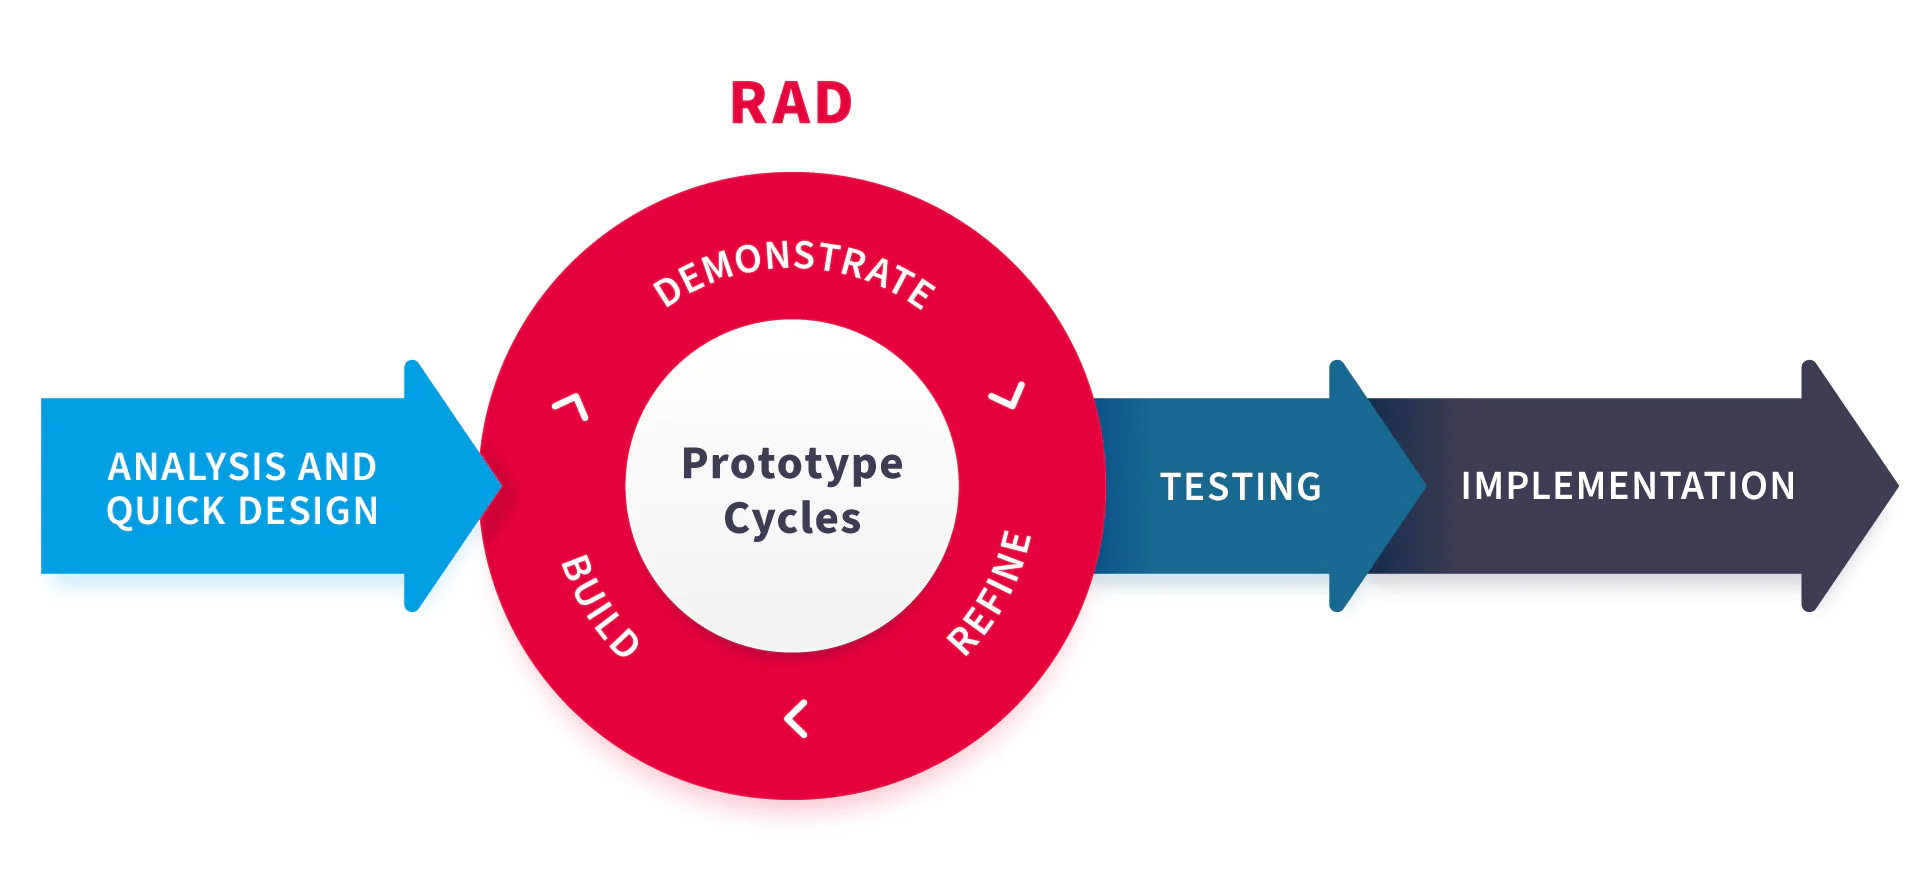
\includegraphics[width=1\linewidth]{figures/images/doc/rad.png}
    \caption{Rapid Application Development (RAD) Model.}
    \label{fig:rad}
\end{figure}
    
\section{System Analysis}
The system analysis phase of the HRIS application development involves utilizing various methods to understand and define the system's functional and data requirements. These include information gathering, analytical methods, personnel consultation assessments, and content analysis. These methods aid in identifying user needs, defining system functionalities, and establishing the database schema. 

Through the use of visual tools i.e., Swim-lane Diagram, Use case Diagrams, Entity Relational Diagrams, and Gantt charts, the system analysis phase enables a comprehensive understanding of the HRIS application's scope and requirements. By employing a systematic approach to system analysis, the development team can ensure that the HRIS application is designed and implemented in alignment with the project objectives and user expectations.

\subsection{Organizational Structure}

The ADNU HRMO currently maintains an organizational structure, with each role clearly defined to ensure efficient management and operation of the HRIS. Each role has specific responsibilities and access levels within the HRIS, ensuring that the system operates smoothly and effectively.

\begin{figure}[H]
    \centering
    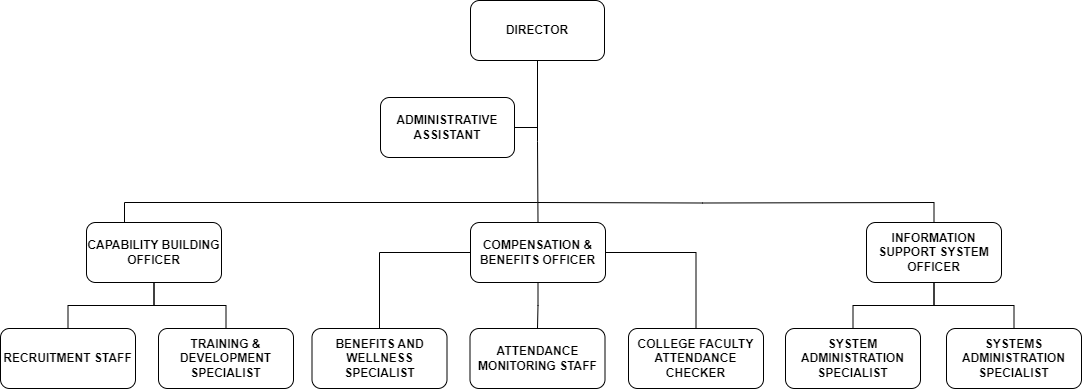
\includegraphics[width=1\linewidth]{figures/images/doc/organizational-structure.png}
    \caption{HRIS Organizational Structure.}
    \label{fig:organizational-struct}
\end{figure}

With this organizational structure in place, the new system will be designed to accommodate the roles and responsibilities of each HR staff member present in the structure figure \ref*{fig:organizational-struct}. 

    \subsection{Swim-lane Diagram}
    The Swim-lane diagram illustrates the process flow of the HRIS. The process begins when the user enters their login credentials. These credentials are unique to each University personnel, distinguishing them from other users in the system. Each user has different privileges and assignments set initially to access the system. After entering the credentials, the system validates them, granting the user access to the system. Once the user successfully logs in, they are directed to the dashboard where they can perform different actions depending on their privileges e.g., perform employee actions or tasks and HR overall general management.

    The identified roles i.e., Director, Sys. Admin, Attendance Monitoring and Checker, Training \& Dev. Specialist, Records Mgt. Specialist, Comp. \& Benefits Officer, ISS Officer, Recruitment \& Admin Staff, and Capability Bldg. Officer, are assigned specific tasks and responsibilities within the system. These responsibilities and privileges are outlined in table \ref*{tab:hris-basic-modules}. 

    \begin{figure}[H]
        \centering
        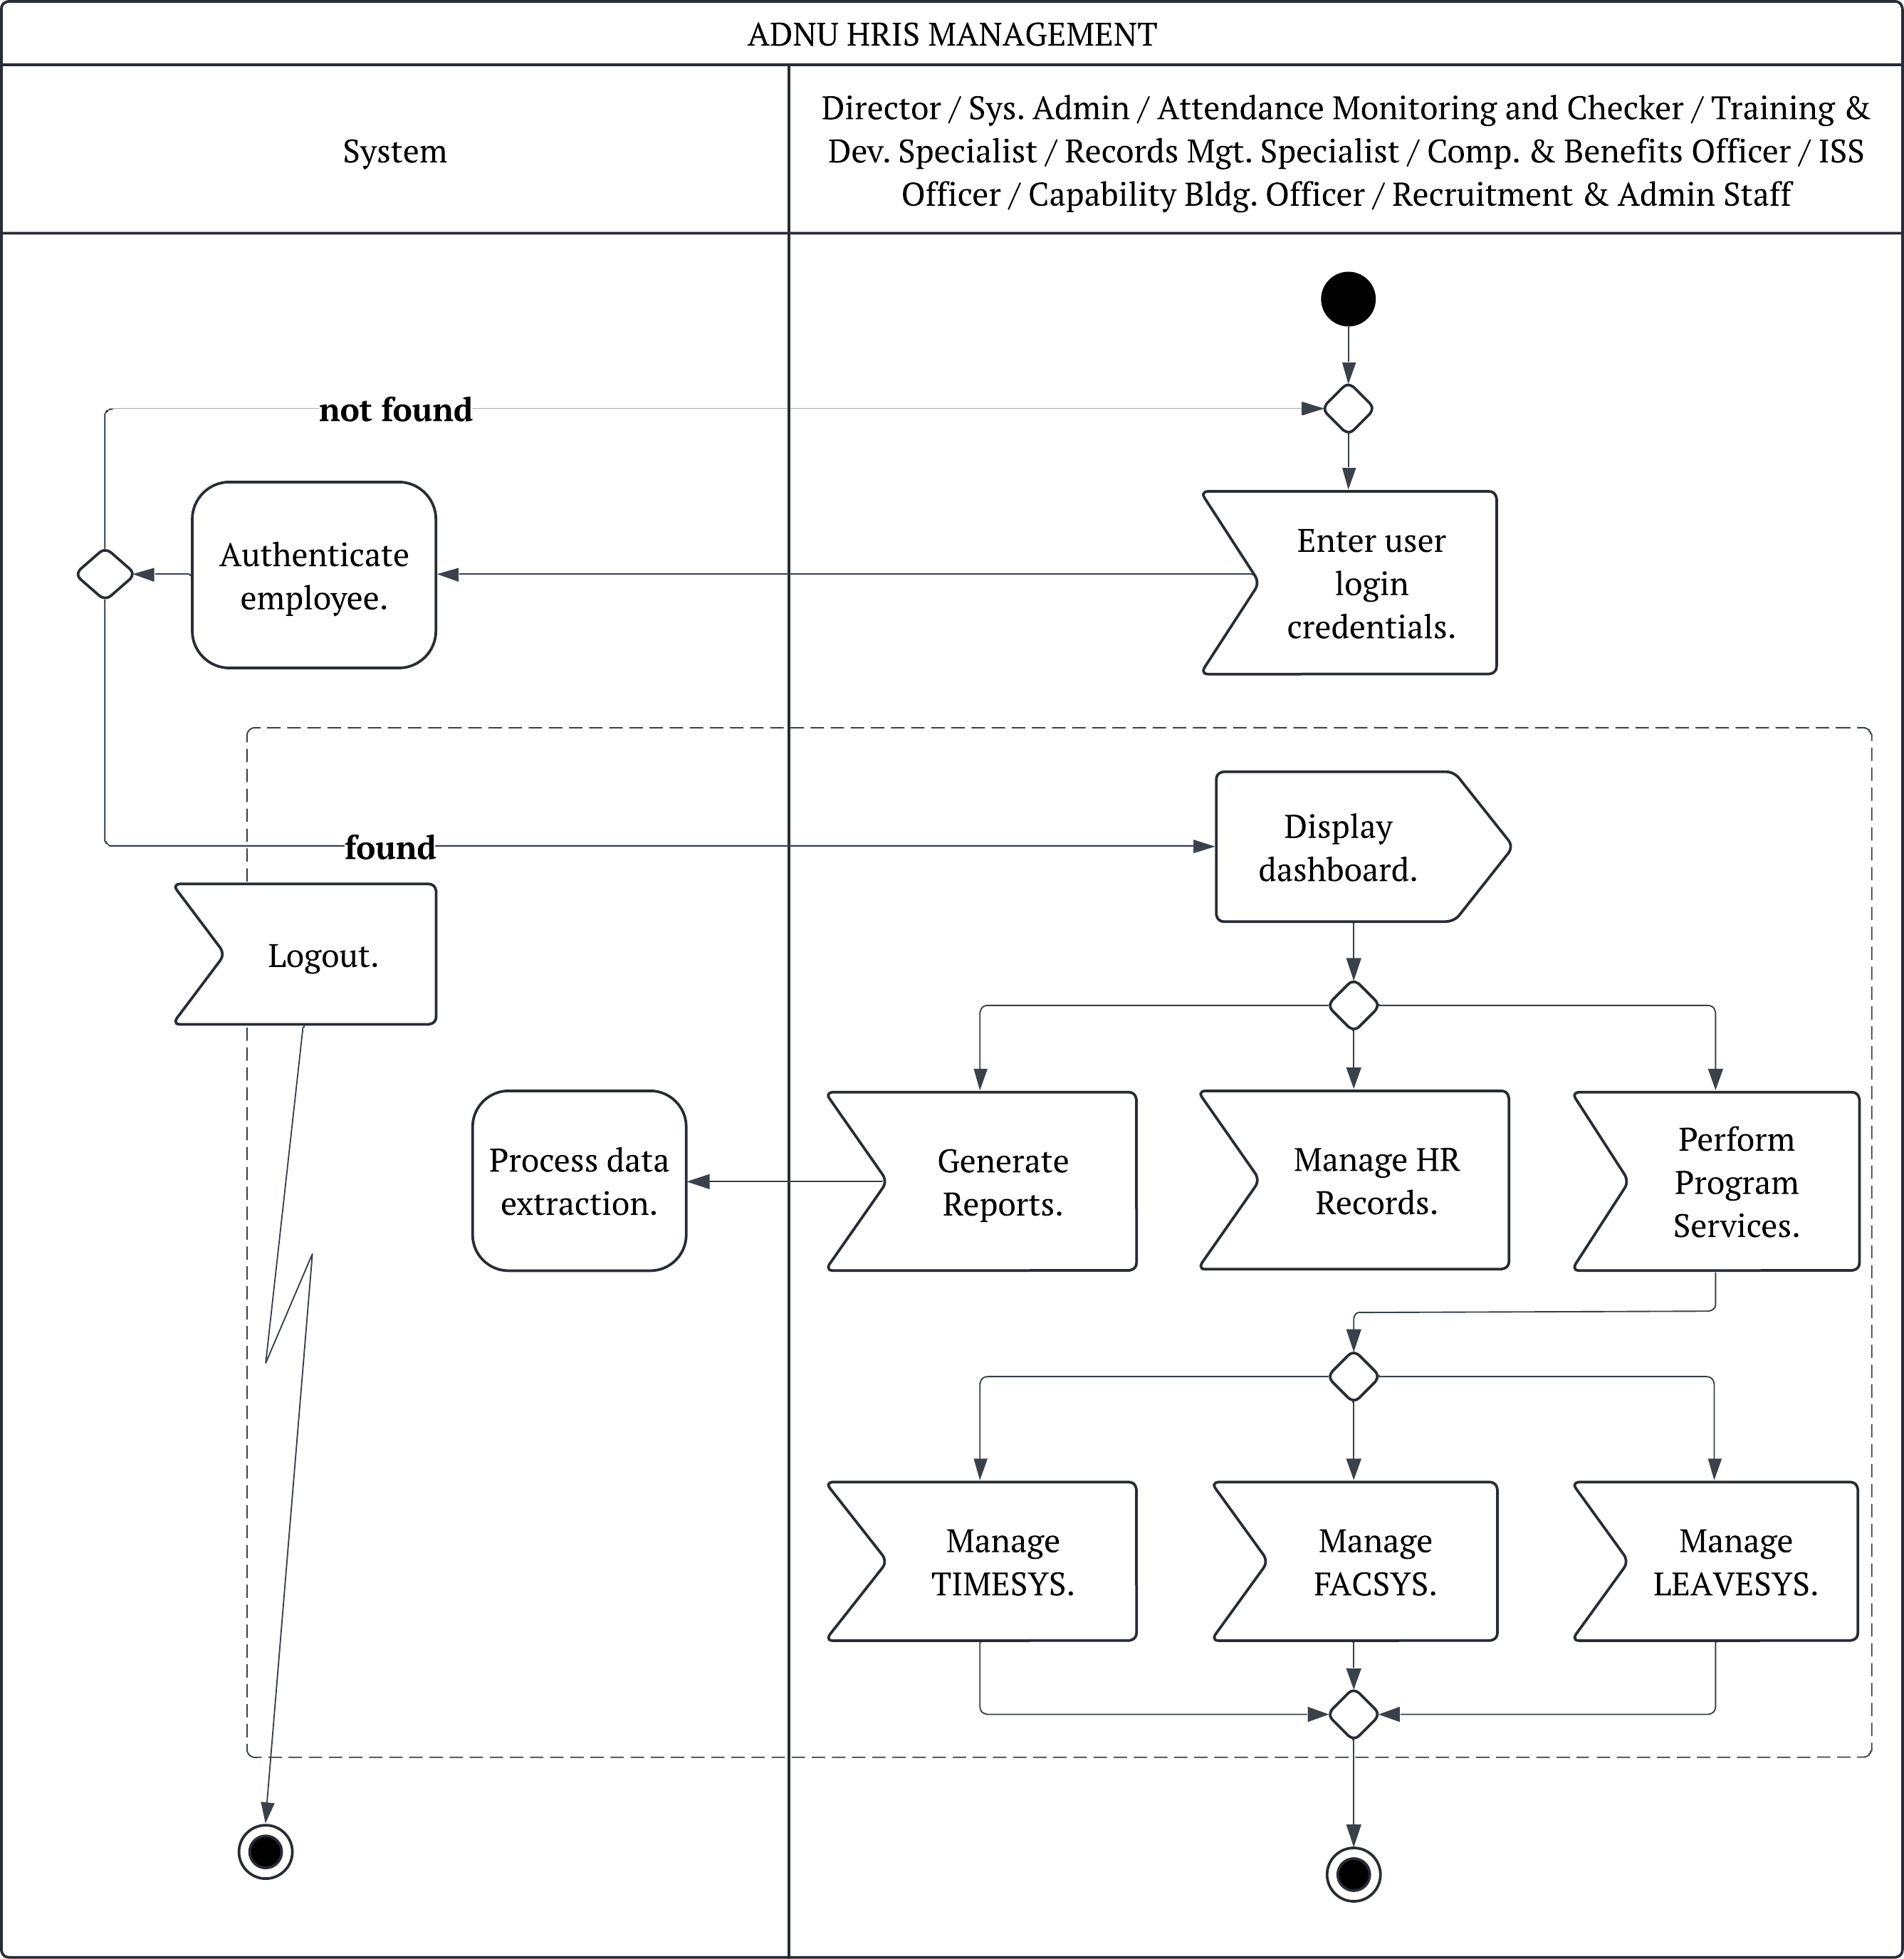
\includegraphics[width=1\linewidth]{figures/images/diagrams/swimlane/swimlane-admins.png}
        \caption{HRIS Swim-lane Diagram Model for HR Management.}
        \label{fig:swimlane-admins}
    \end{figure}

    Each role area can perform admin privileges and manage different modules within the system. For these actions, they are processed and managed under the system to provide a streamlined operation for any users in the system. Higher admins will have access to core modules e.g., Manage employee/personnel containing the employee contacts, personal information, profiles, assignments, assignment archive, faculty rank, academic, academic awards, professional license, training attendance, Certificate of Employment (COE), and health record.

    Besides this, these admins can also generate different kinds of reports within the system e.g., performing data extraction, queries, employee performance evaluation, COE reports, contracts/appointment generation, etc.

    \begin{figure}[H]
        \centering
        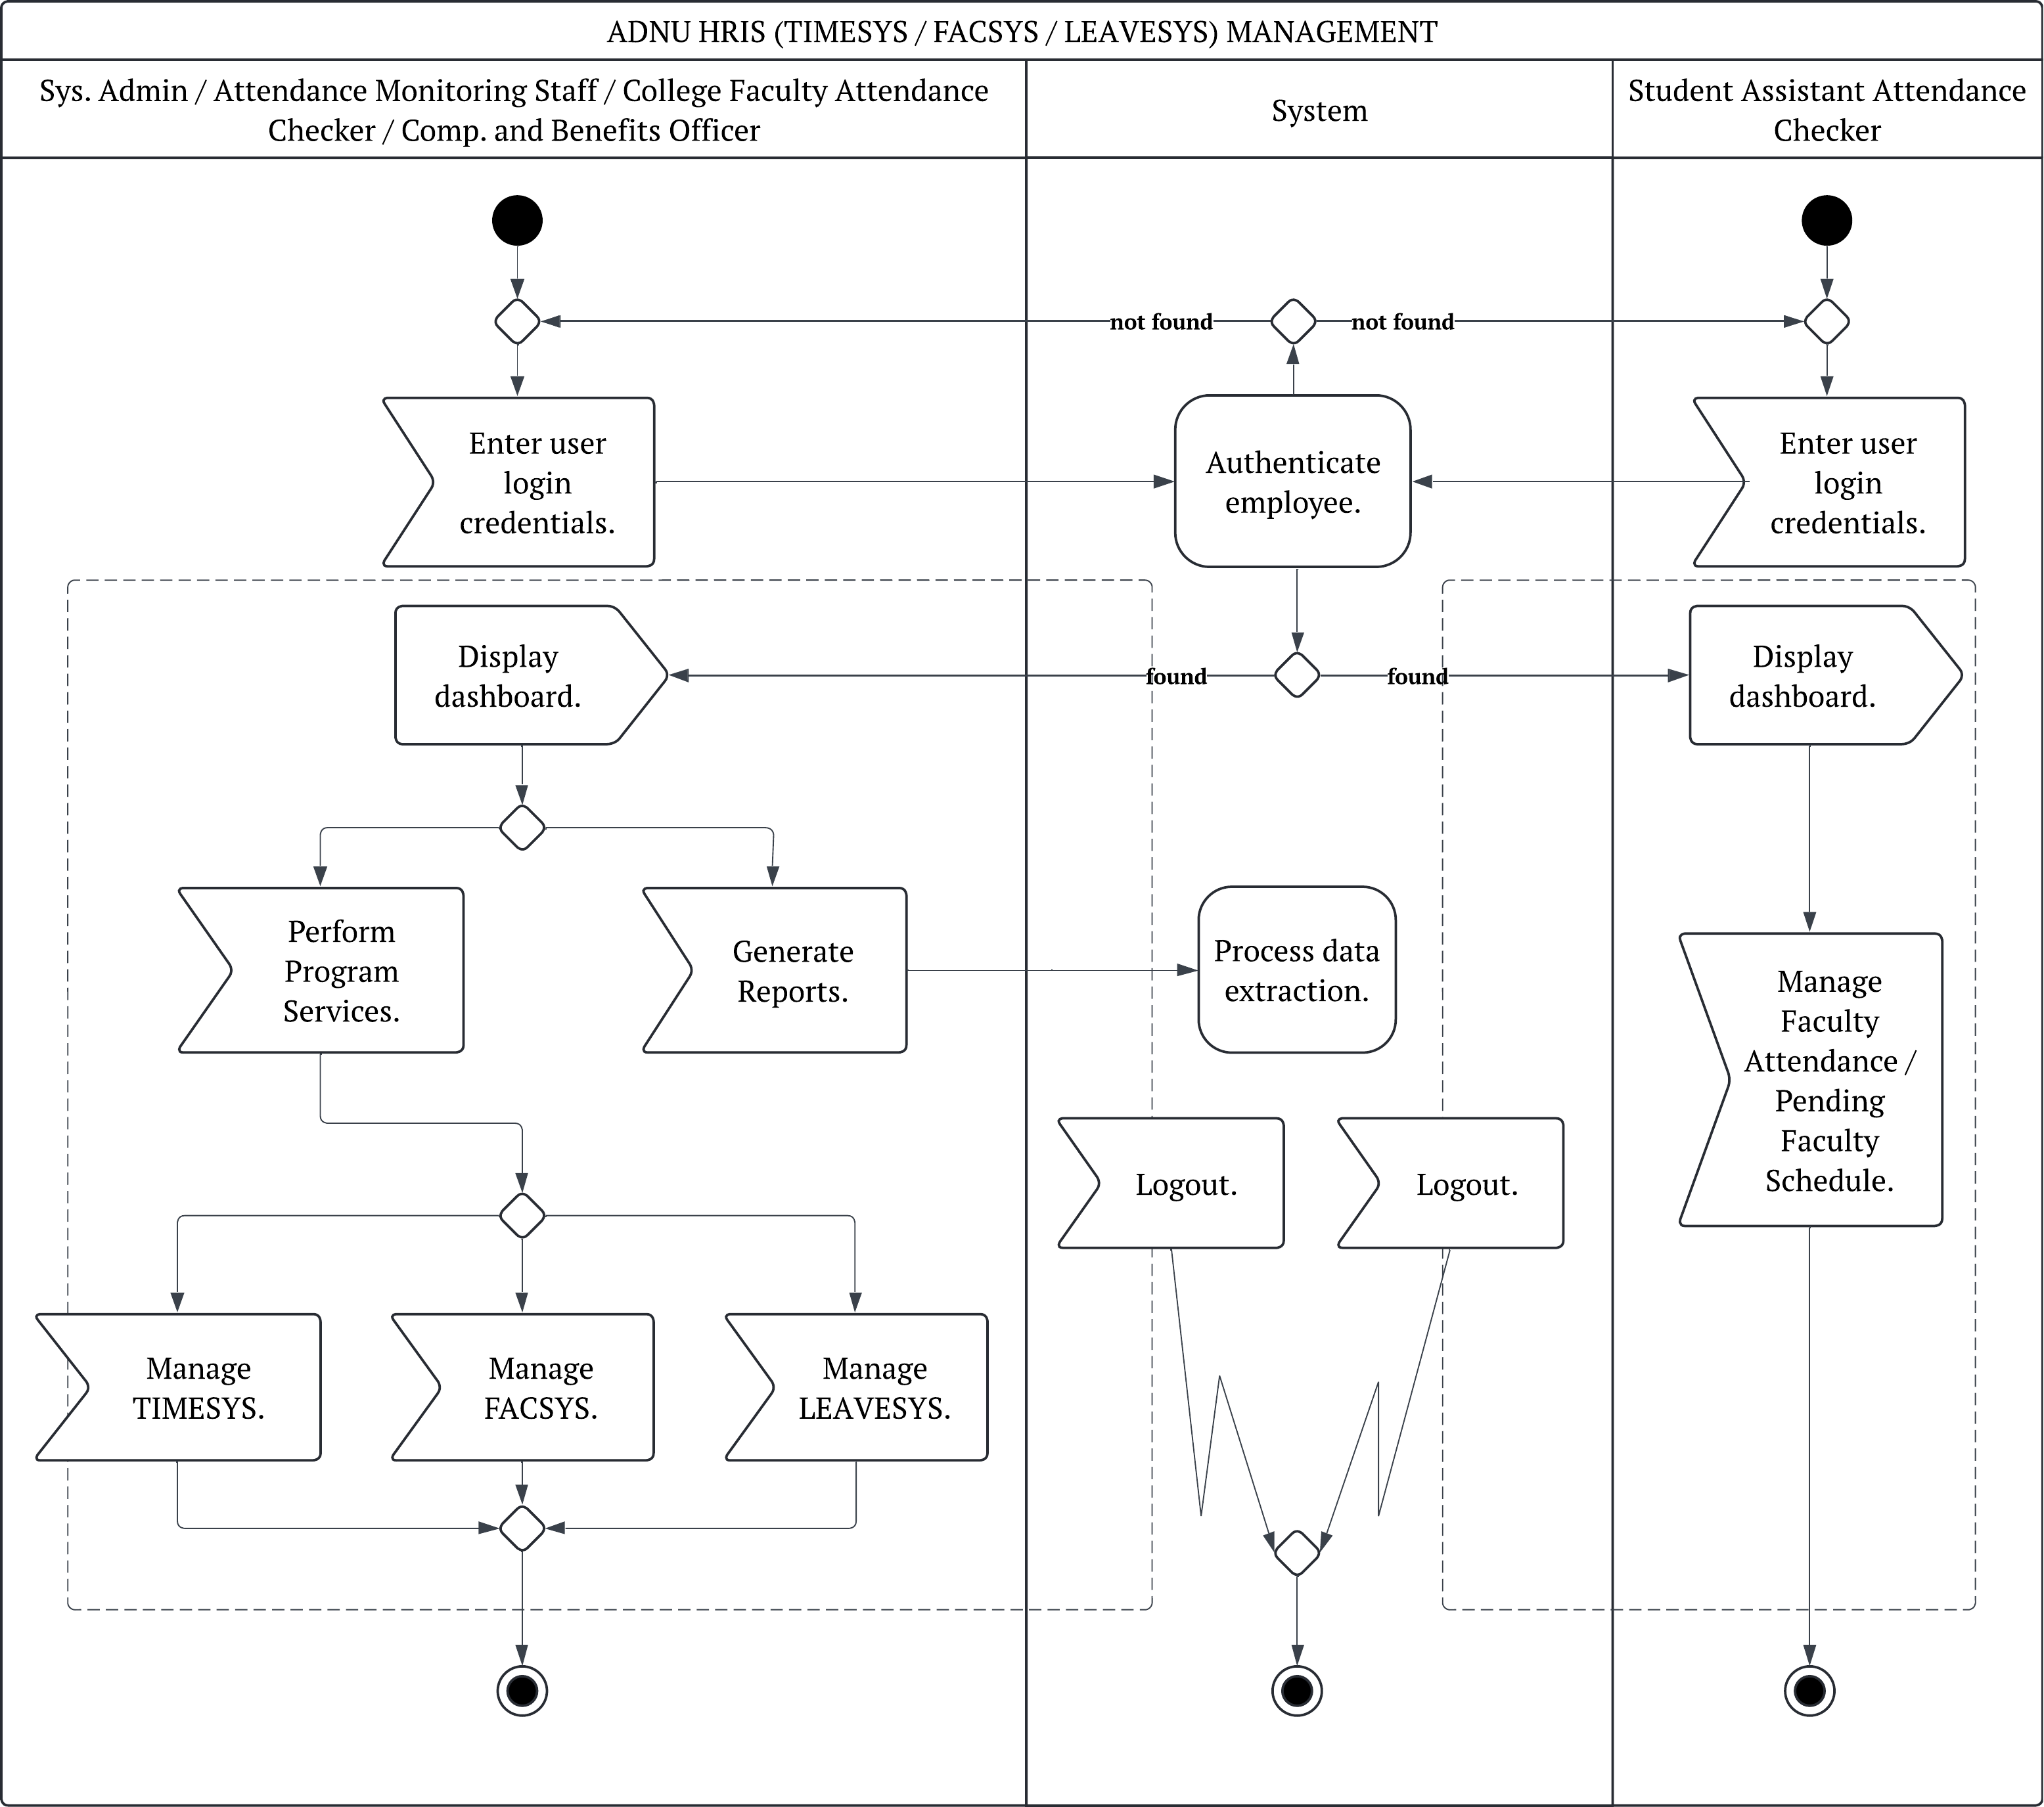
\includegraphics[width=1\linewidth]{figures/images/diagrams/swimlane/swimlane-sys-mgt.png}
        \caption{HRIS Swim-lane Diagram Model for TIMESYS, FACSYS, and LEAVESYS Management.}
        \label{fig:swimlane-sys-mgt}
    \end{figure}

    The system also includes modules for TIMESYS, FACSYS, and LEAVESYS. These modules are designed to manage employee attendance, faculty attendance, and employee leave applications, respectively. In the diagram, the identified roles along with their privilege are assigned to manage the three (3) SYS as well as allowing them to generate reports. Meanwhile, the Student Assistant Attendance Checker has lesser privilege and is assigned only to managing faculty attendance, faculty schedule, and managing pending faculty schedules.

    \subsection{Use Case Diagram}
    
    The use case diagram serves as a visual representation of the functional requirements of the system from an external user's perspective. It illustrates the interactions between users and the system, showcasing the various use cases and how they relate to each other. Each module referred to in \ref*{tab:hris-basic-modules}, \ref*{tab:hris-facsys-modules}, \ref*{tab:hris-leavesys-modules}, \ref*{tab:hris-timesys-modules} has specific use cases that define the functionalities and interactions within the system. Moreover, each module has different actors with specific roles and access levels, allowing for a comprehensive overview of the system's behavior and user interactions.
    
    Additionally, the concept of 'Manage' refers to the access users have to create, view, edit, and archive data or information within specific modules, By mapping out these interactions and incorporating both 'Manage' and 'View' functionalities, the use case diagram helps in identifying the system's behavior and the roles of different users in the HRIS application.

    In the HRIS Basic Modules Use Case Diagram, alongside Performing Data Extraction and Managing/Viewing Performance Evaluation, the use cases are grouped into four primary functional areas: Employee Information Access, Employment and Assignment Access, Academic and Professional Development Access, and Certification and Reporting Access. Each area extends to specific management or viewing capabilities. Employee Information Access covers personal data, profiles, health records, and professional licenses. Employment and Assignment Access encompasses employee assignments, their archives, and status information. Academic and Professional Development Access includes academic records, awards, and attended training sessions. Lastly, Certification and Reporting Access handles COE (Certificate of Employment) requests, reports, and contracts/appointments generation. This structure allows for efficient organization of various HRIS functions, providing comprehensive coverage of employee-related data management and access across different aspects of human resource operations.

    \begin{figure}[H]
        \centering
        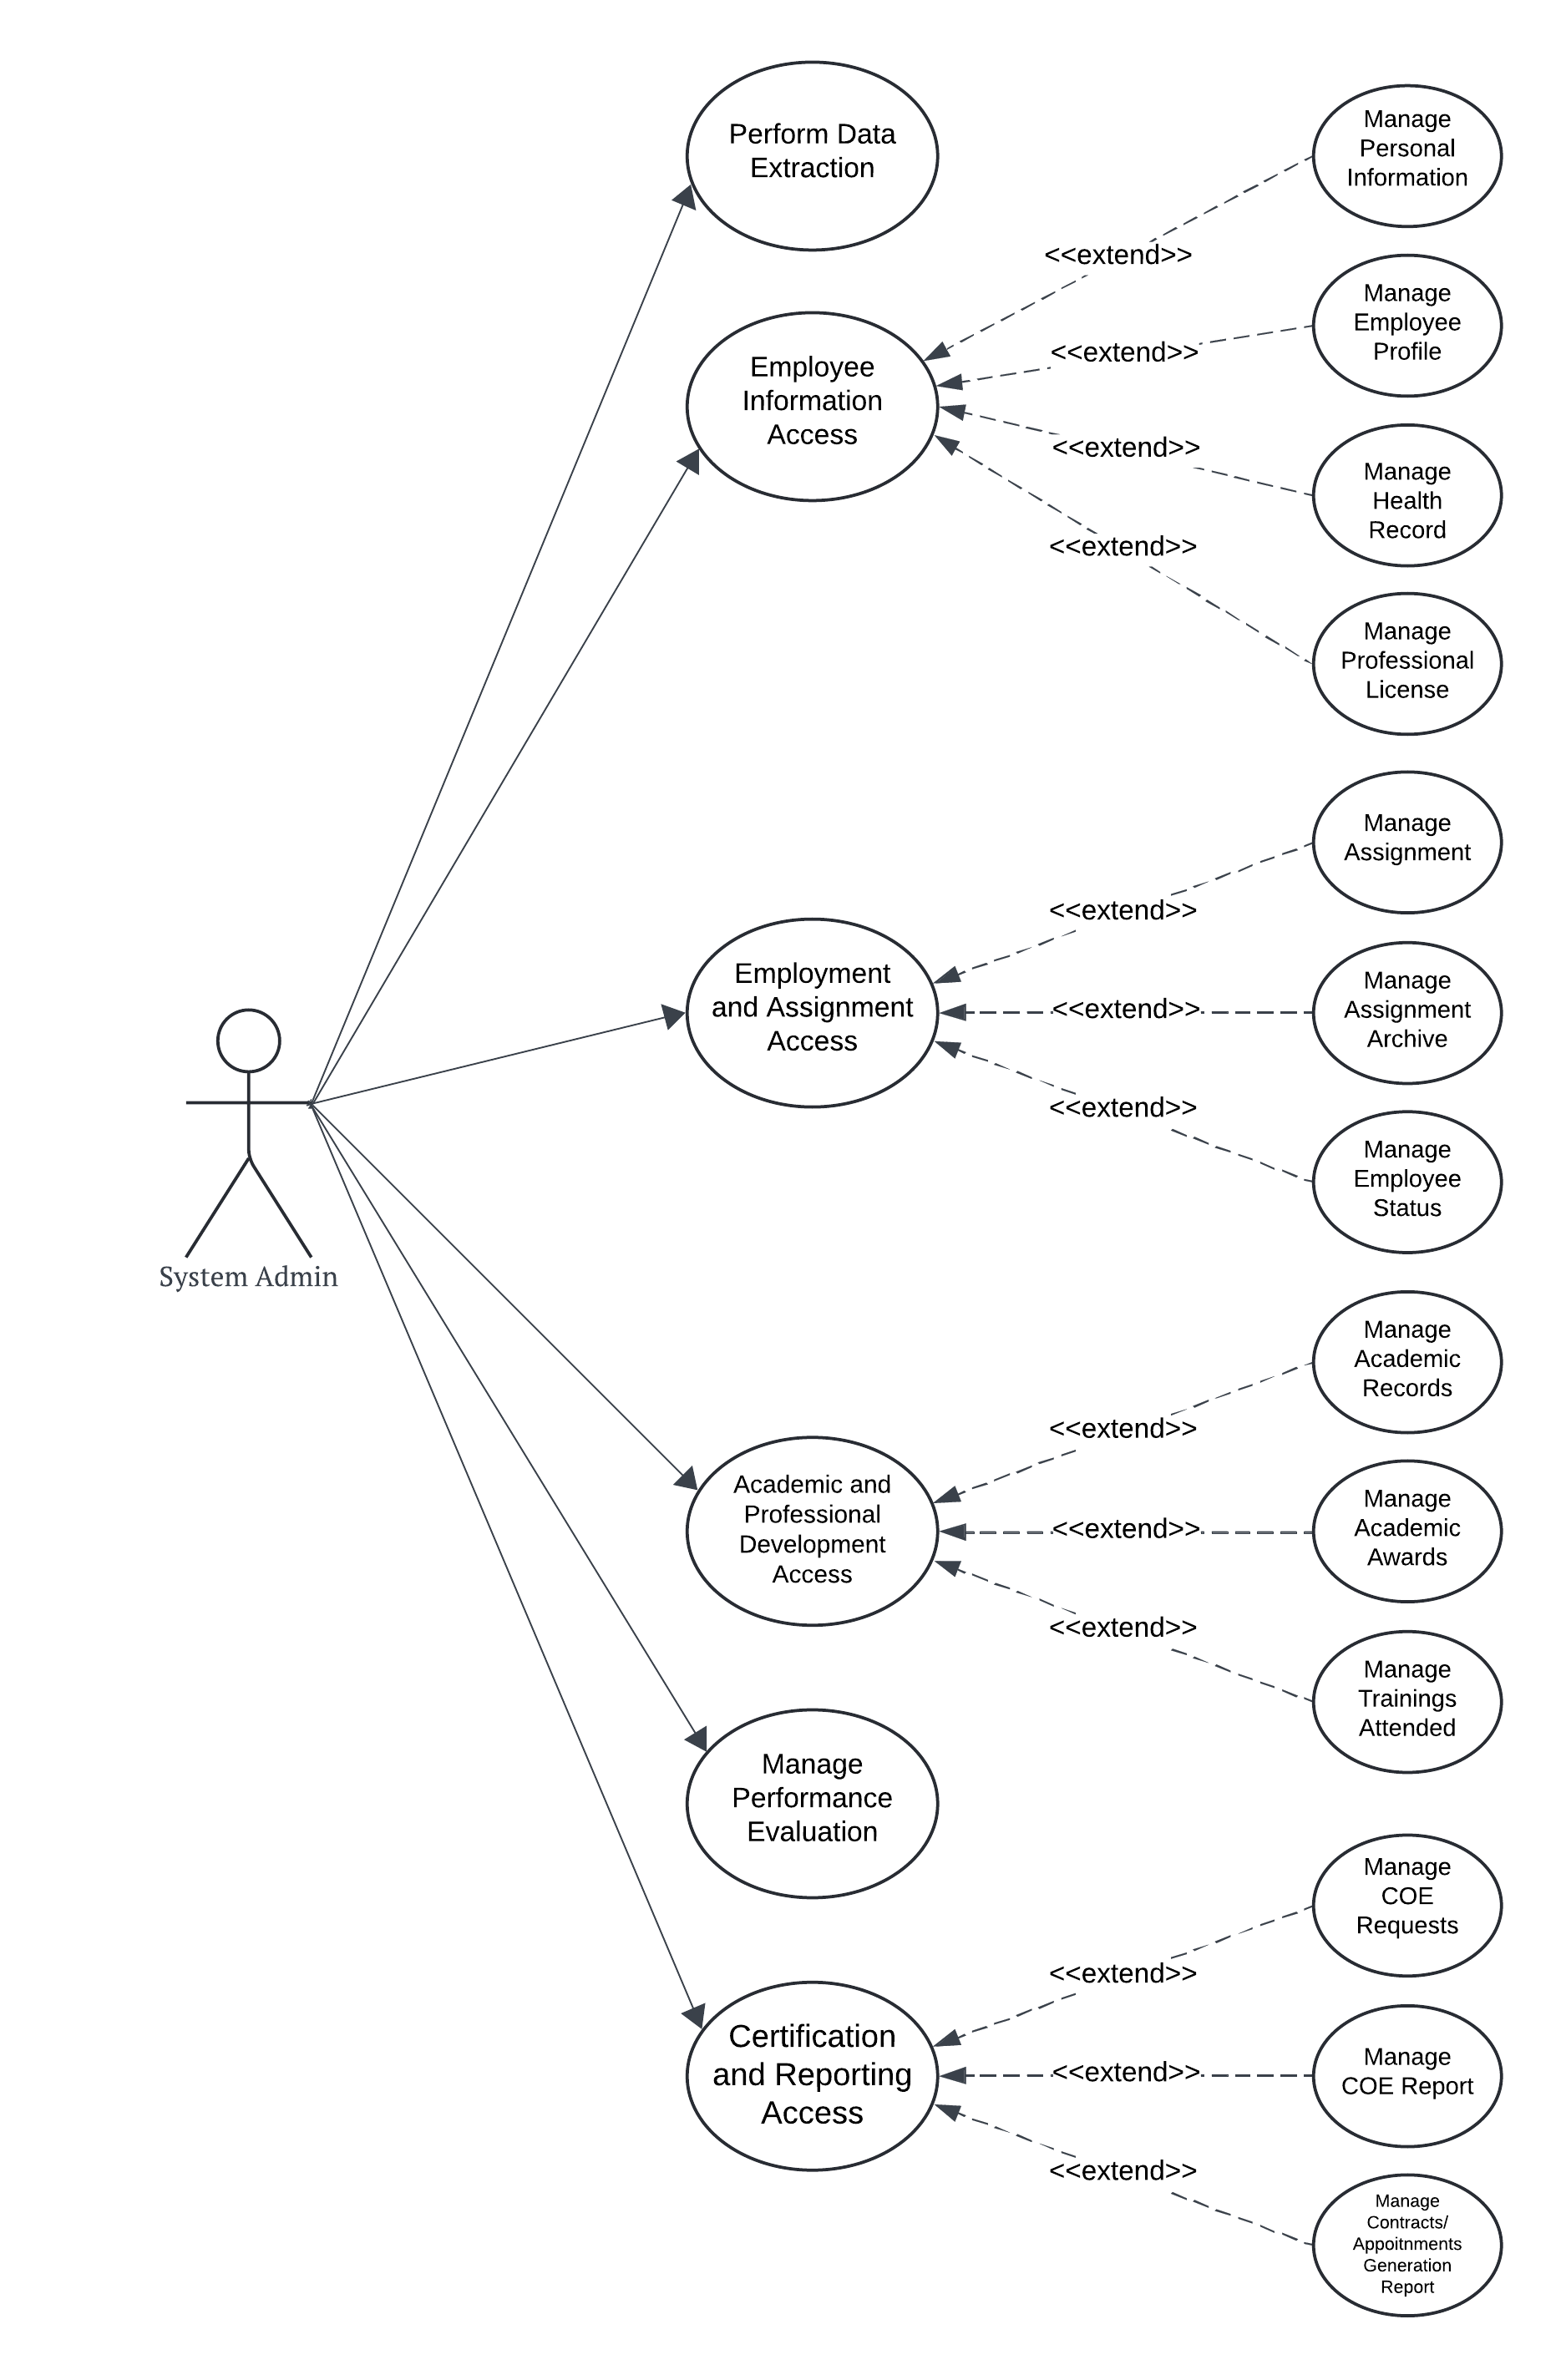
\includegraphics[width=0.9\linewidth]{figures/images/diagrams/usecase/use-case-basic-1.png}
        \caption{HRIS Basic Modules Use Case Diagram: System Admin.}
        \label{fig:use-case-basic-1}
    \end{figure}

    The figure \ref{fig:use-case-basic-1} shows the use case diagram for the System Admin within the HRIS Basic Modules. The System Admin has full managing access to all use cases. This includes Performing Data Extraction, Managing Performance Evaluation and all the modules that encompasses the 4 functional areas: Employee Information Access, Employment and Assignment Access, Academic and Professional Development Access, and Certification and Reporting Access. This comprehensive access enables the System Admin to oversee and manage all aspects of the HRIS application, ensuring efficient and effective HR operations.

    \begin{figure}[H]
        \centering
        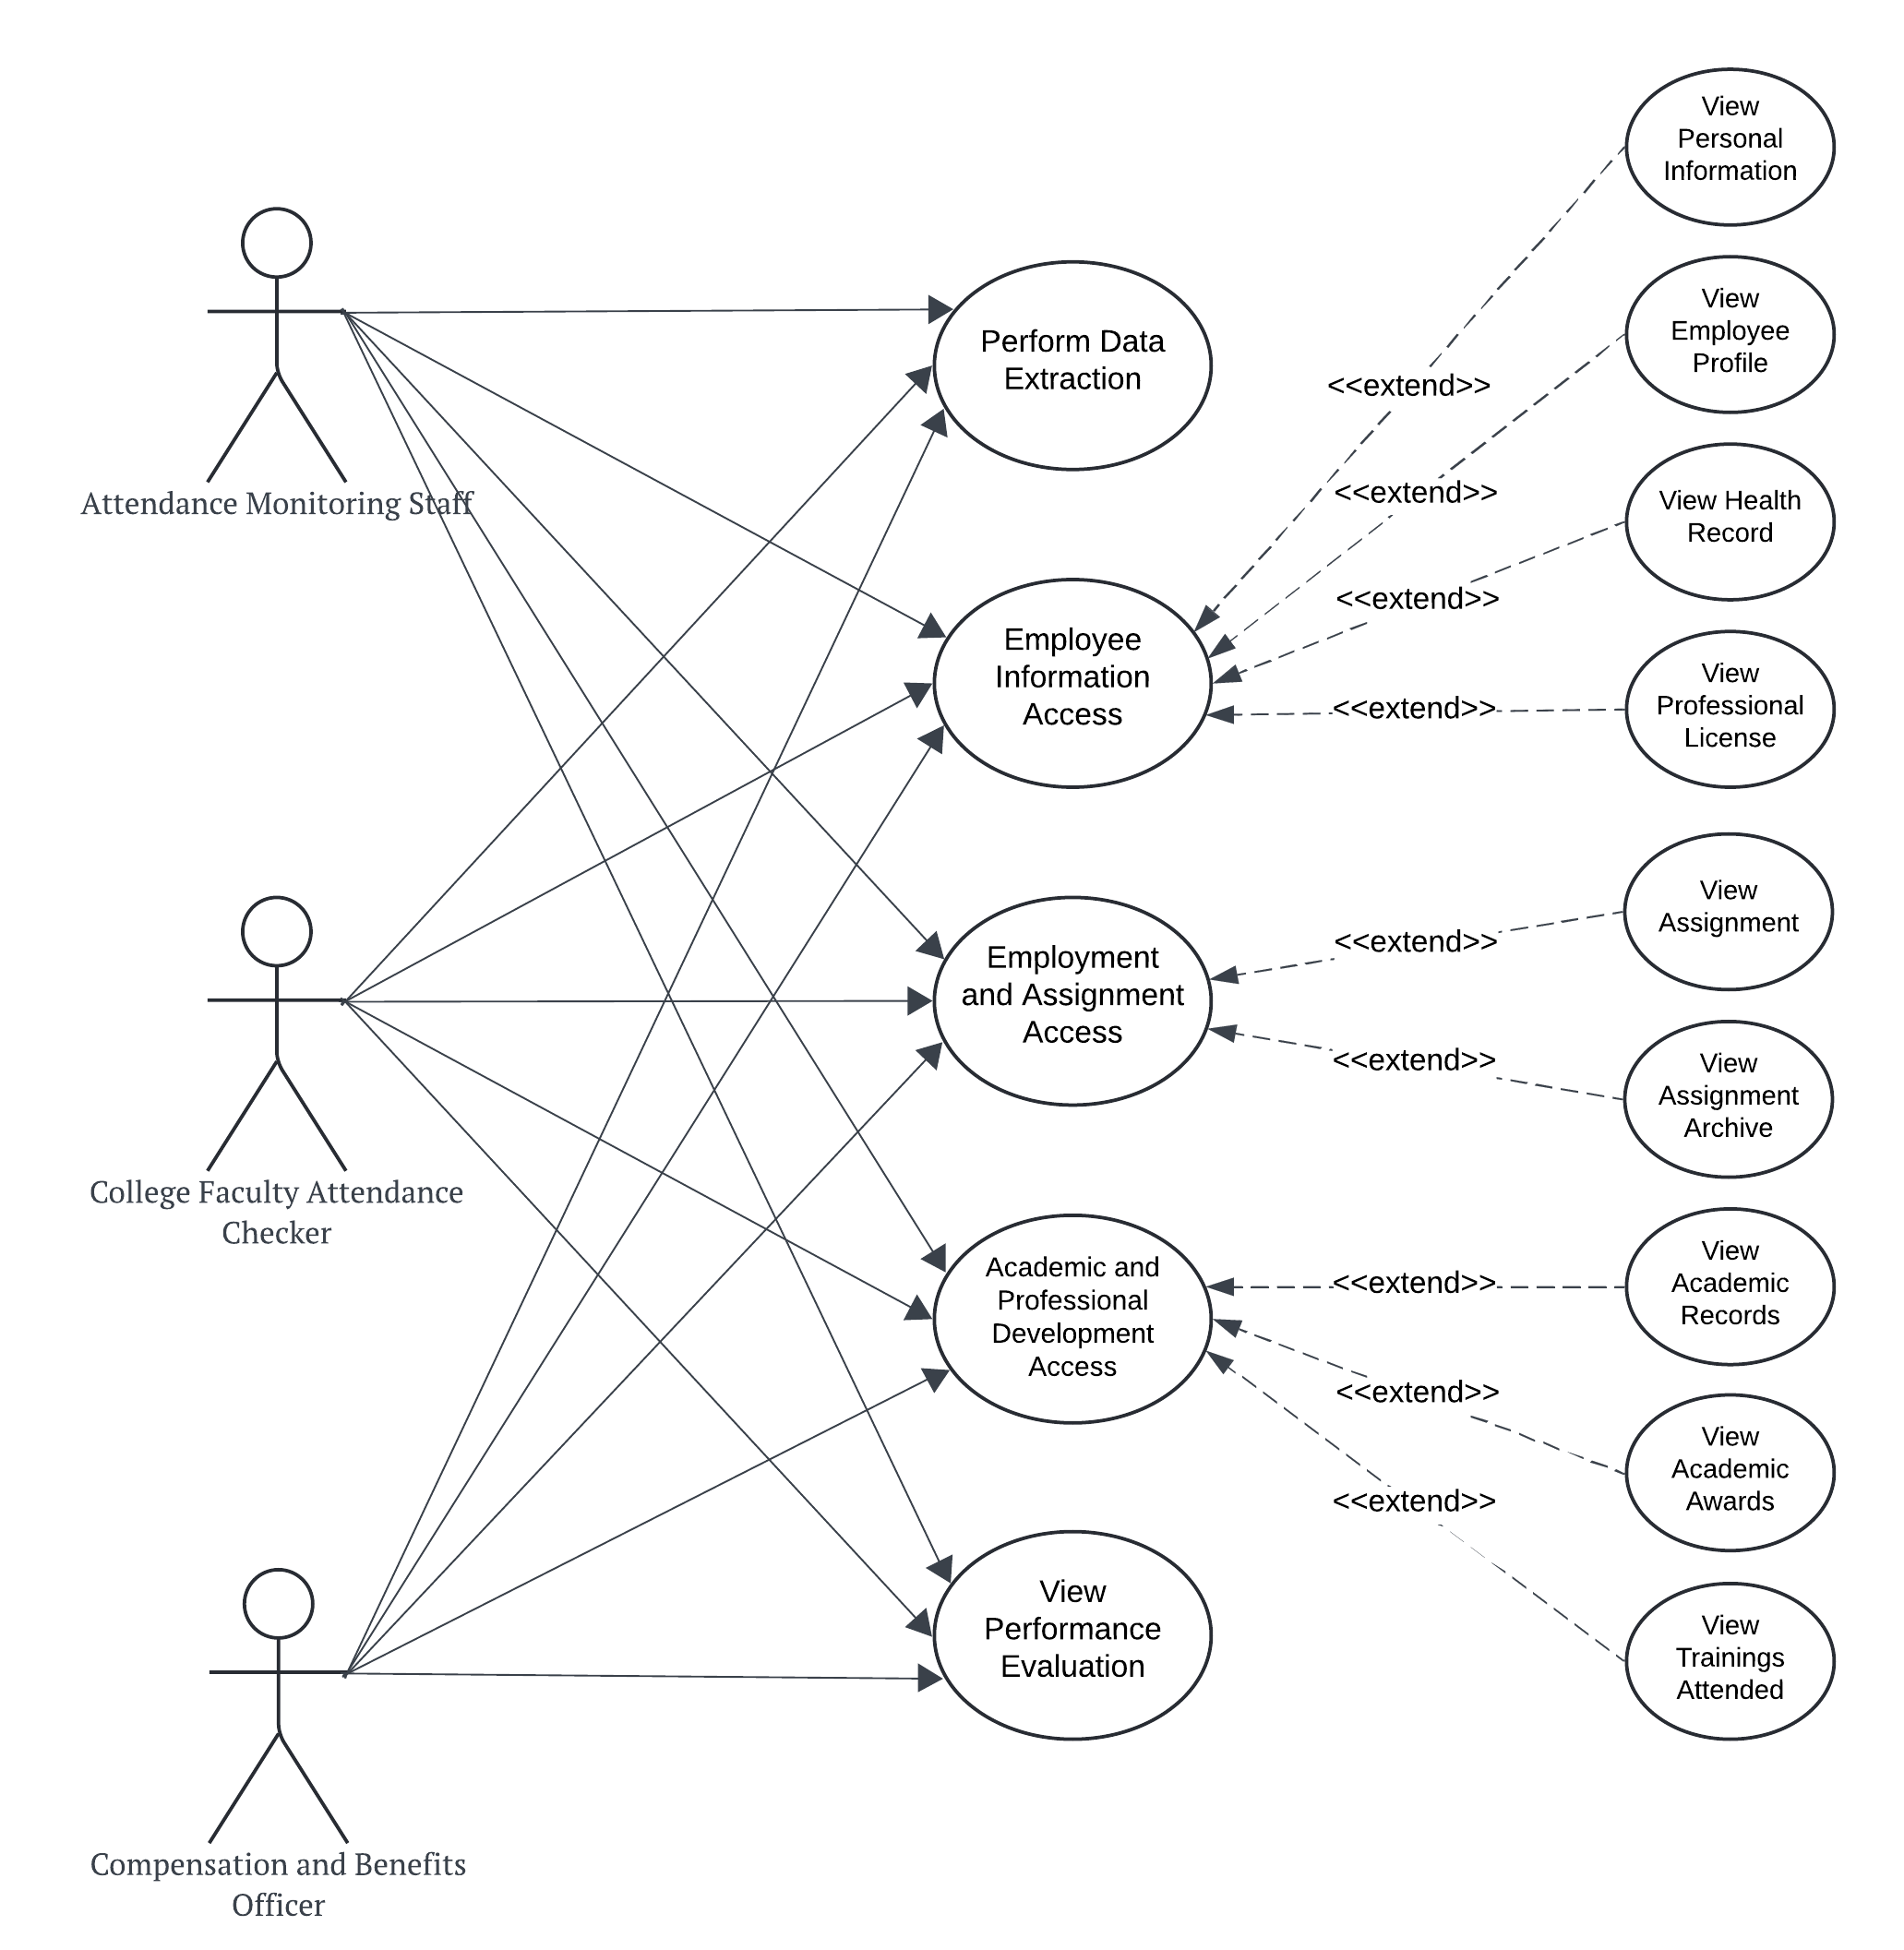
\includegraphics[width=0.9\linewidth]{figures/images/diagrams/usecase/use-case-basic-2.png}
        \caption{HRIS Basic Modules Use Case Diagram: Attendance Monitoring Staff, College Faculty Attendance Checker, and Compensation and Benefits Officer.}
        \label{fig:use-case-basic-2}
    \end{figure}

    The figure \ref{fig:use-case-basic-2} depicts the use case diagram for Attendance Monitoring Staff, College Faculty Attendance Checker, and Compensation and Benefits Officer within the HRIS Basic Modules. These three actors share identical access which is limited to view-only across most use cases. This includes Performing Data Extraction, Viewing Performance Evaluation, and all the use cases that encompasses the 3 functional areas: Employee Information Access, Employment and Assignment Access, and Academic and Professional Development Access. 

    \begin{figure}[H] 
        \centering
        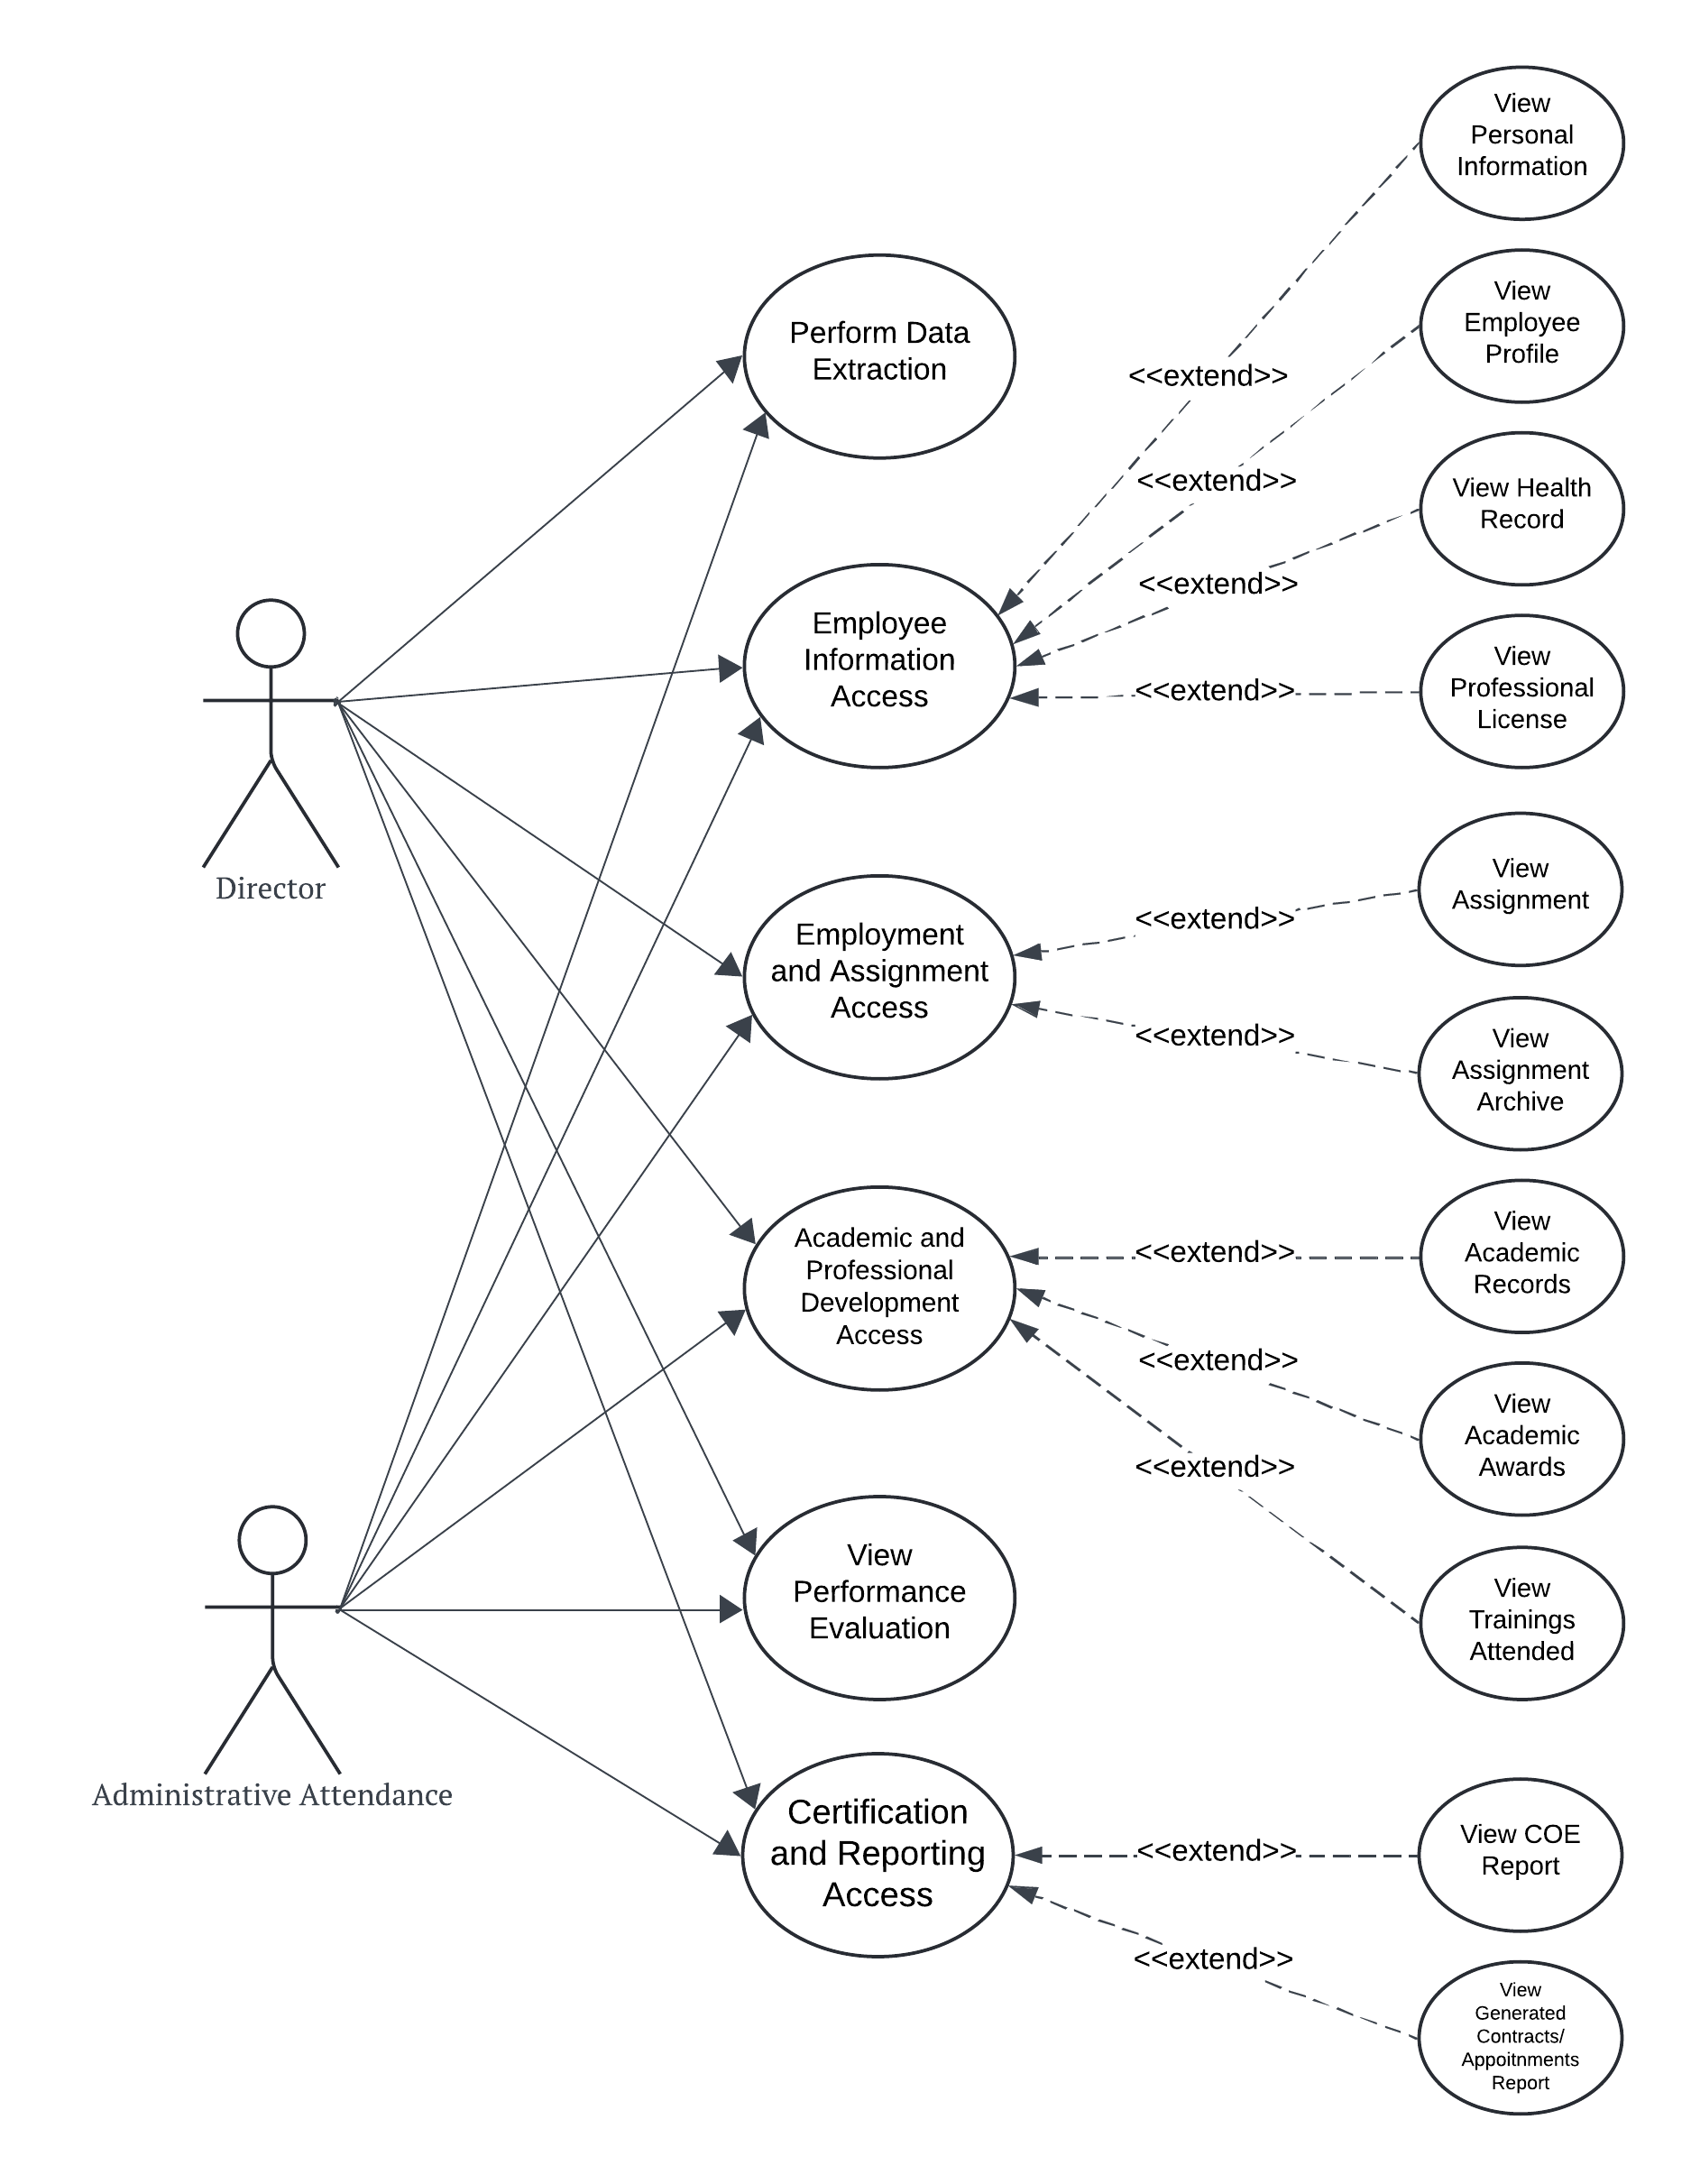
\includegraphics[width=0.9\linewidth]{figures/images/diagrams/usecase/use-case-basic-3.png}
        \caption{HRIS Basic Modules Use Case Diagram: Director and Administrative Assistant.}
        \label{fig:use-case-basic-3}
    \end{figure}

    The figure \ref{fig:use-case-basic-3} shows the use case diagram for the Director and Administrative Assistant within the HRIS Basic Modules. Both actors share access which is limited to view-only across all the use cases. This includes Performing Data Extraction, Viewing Performance Evaluation, and all the use cases that encompasses the 4 functional areas: Employee Information Access, Employment and Assignment Access, Academic and Professional Development Access, and Certification and Reporting Access. 

    \begin{figure}[H]
        \centering
        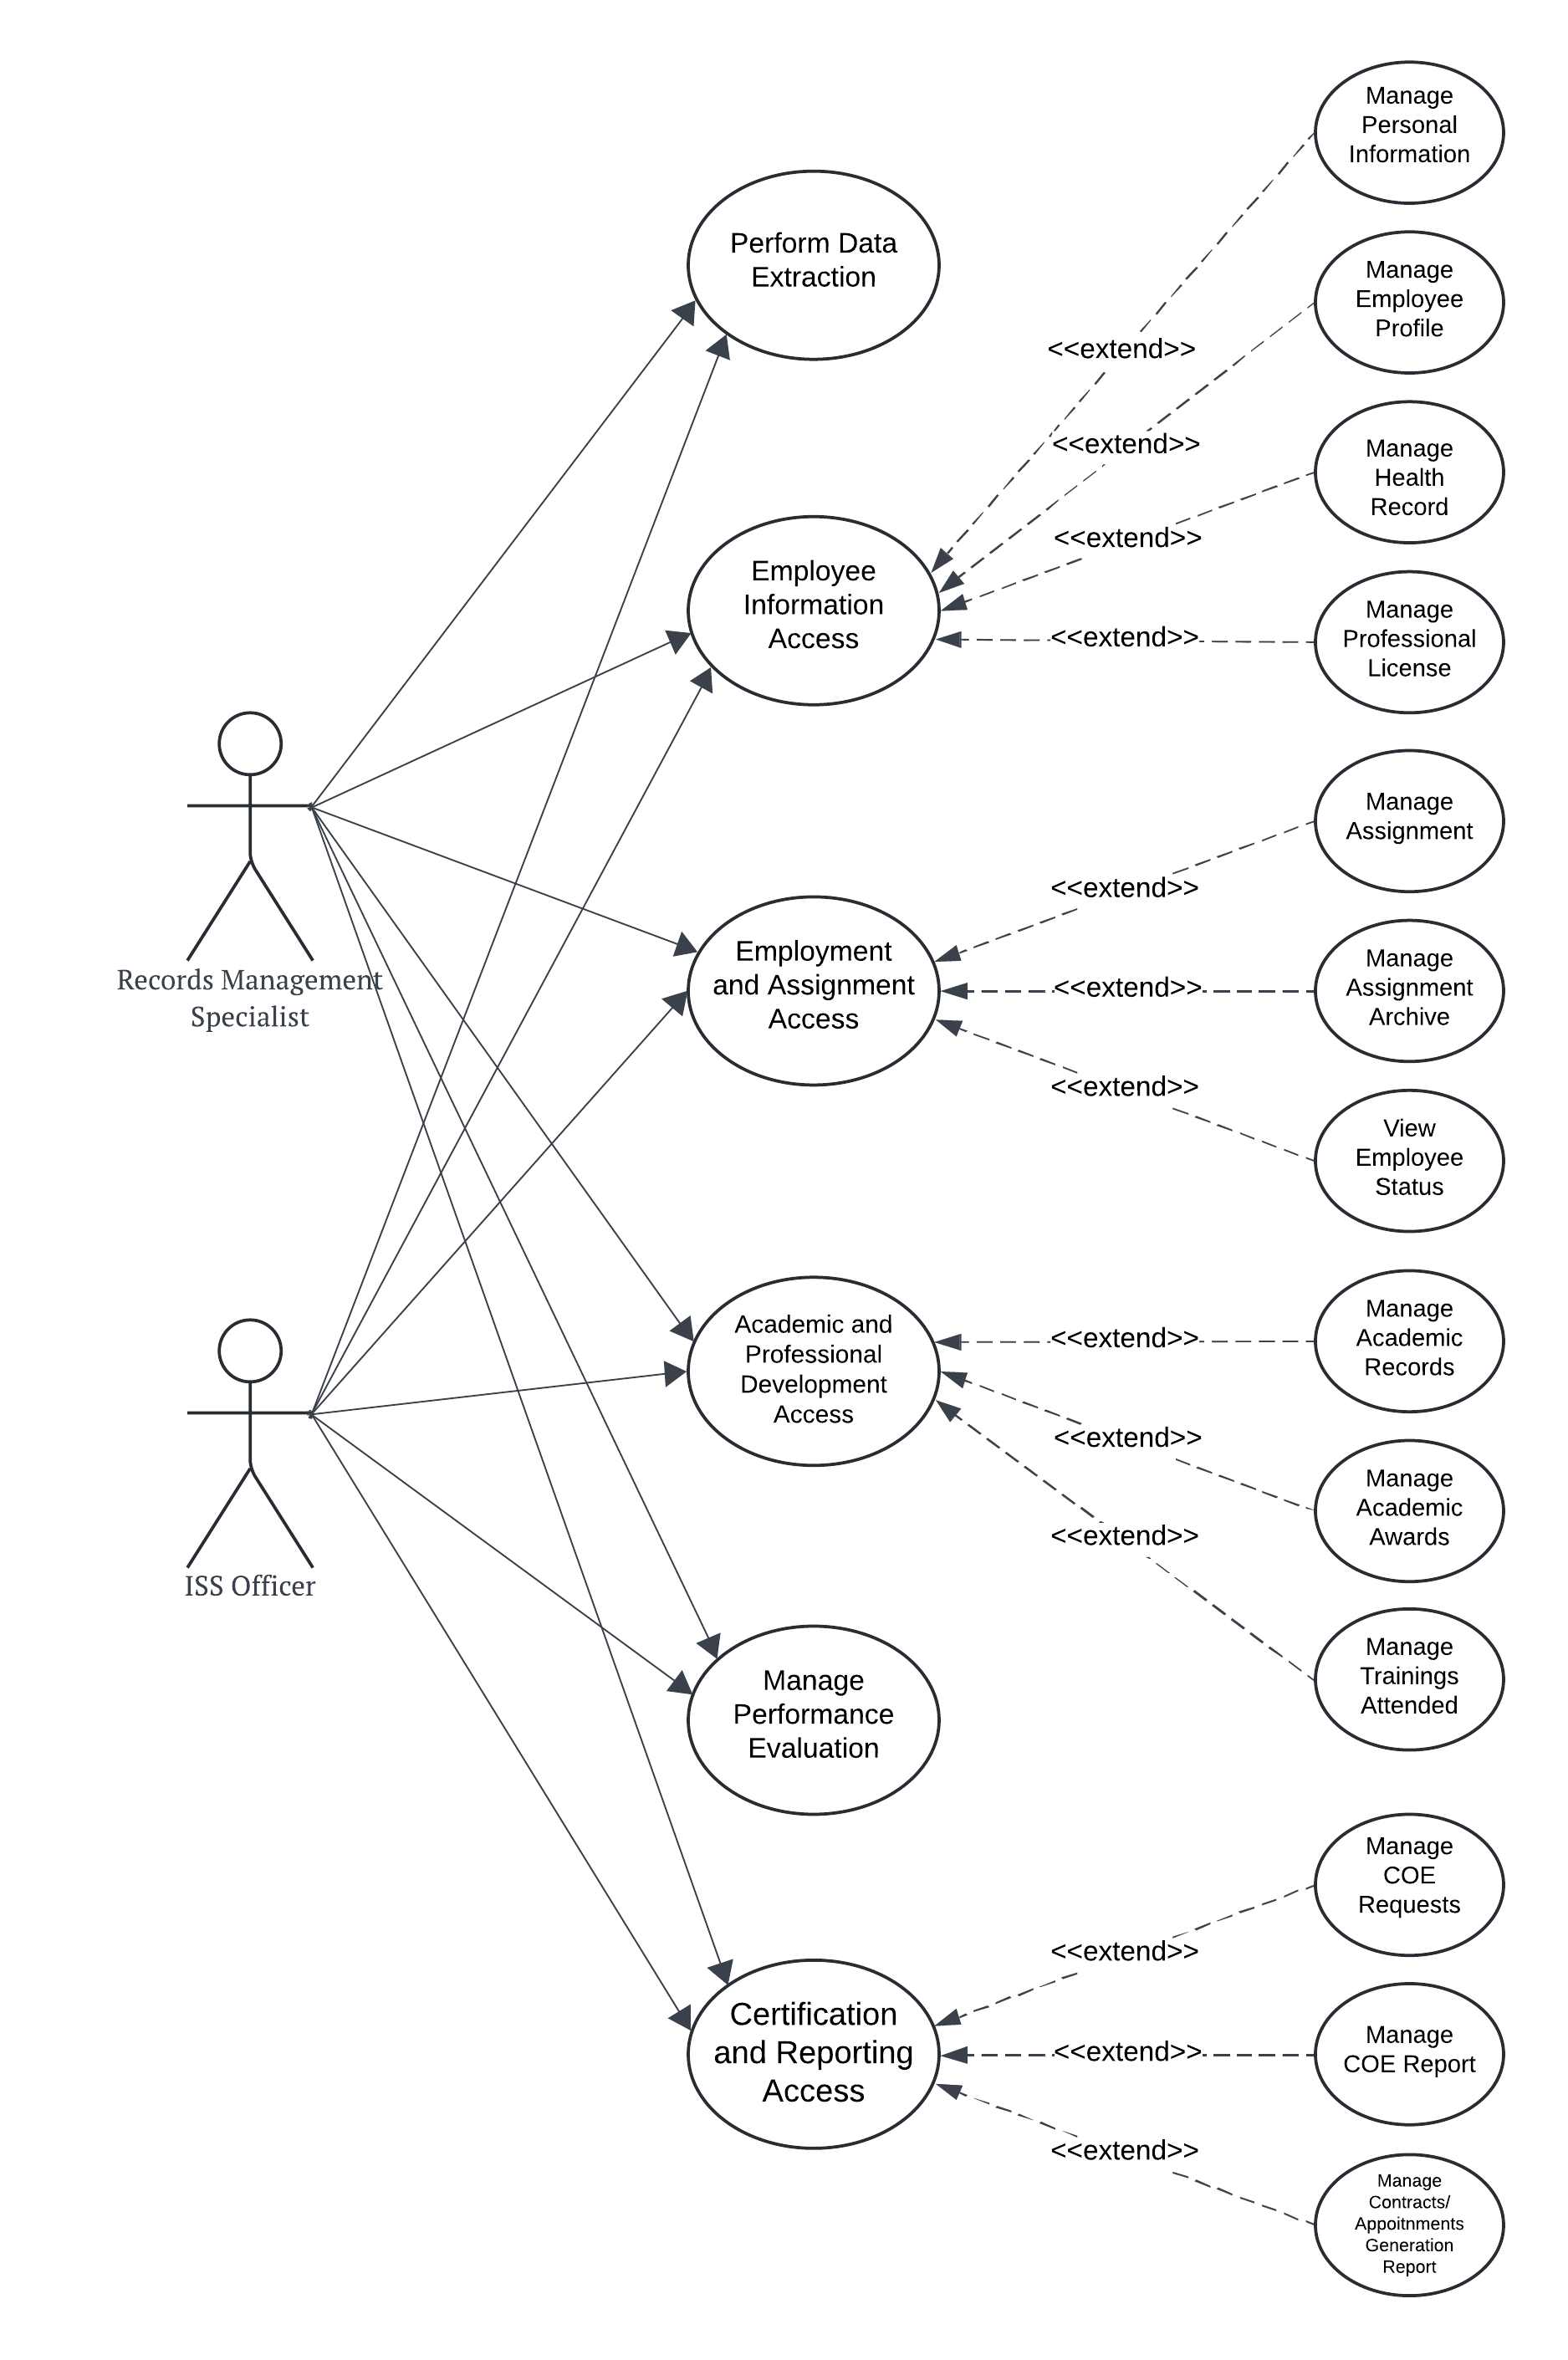
\includegraphics[width=0.9\linewidth]{figures/images/diagrams/usecase/use-case-basic-4.png}
        \caption{HRIS Basic Modules Use Case Diagram: Records Management Specialist and ISS Officer.}
        \label{fig:use-case-basic-4}
    \end{figure}

    The figure \ref{fig:use-case-basic-4} illustrates the use case diagram for the Records Management Specialist and ISS Officer.Both actors share the same access to the HRIS Basic Modules which is managing access to all use cases except one. This includes Performing Data Extraction, Managing Performance Evaluation, and all the use cases that encompasses the 4 functional areas: Employee Information Access, Employment and Assignment Access, Academic and Professional Development Access, and Certification and Reporting Access. The only exception is that, both actors can only view the employee status found in the Employment and Assignment Access functional area.

    \begin{figure}[H]
        \centering
        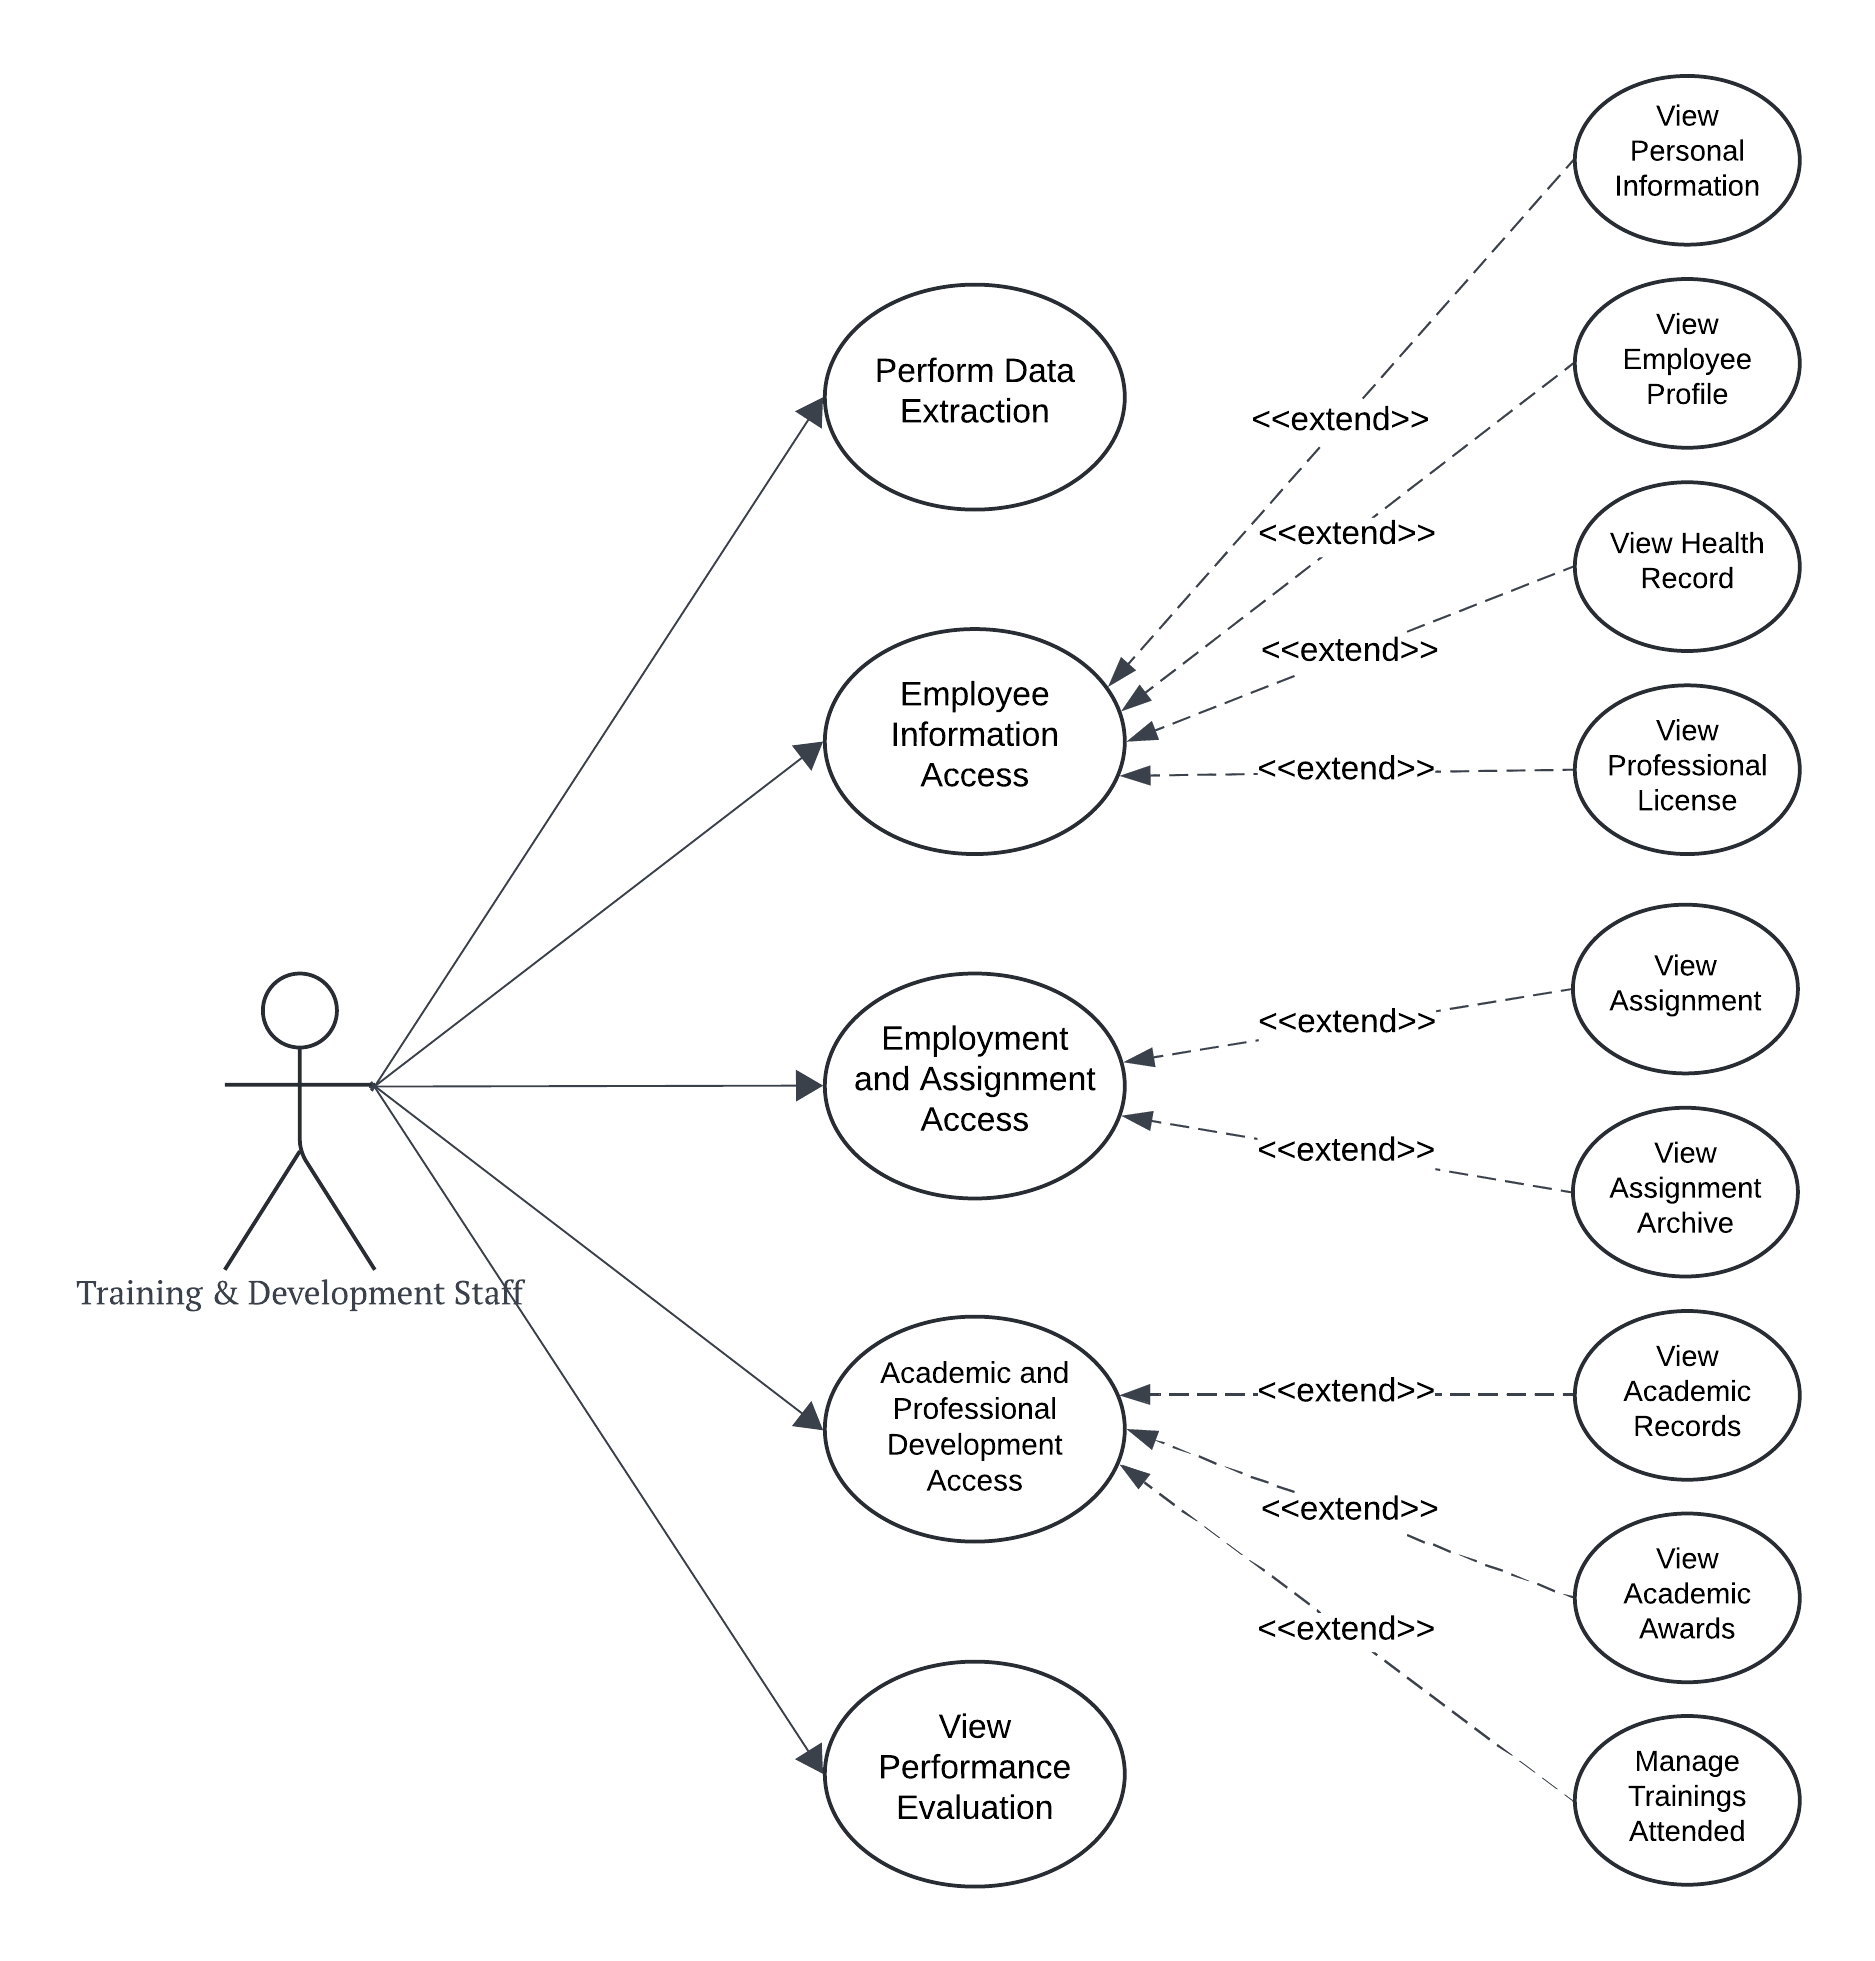
\includegraphics[width=0.9\linewidth]{figures/images/diagrams/usecase/use-case-basic-5.png}
        \caption{HRIS Basic Modules Use Case Diagram: Training and Development Staff.}
        \label{fig:use-case-basic-5}
    \end{figure}
    
    The figure \ref{fig:use-case-basic-5} demonstrates the use case diagram for the Training and Development Staff within the HRIS Basic Modules. The actor has limited view access to the most of the use cases. This includes Performing Data Extraction, Viewing Performance Evaluation, and also the use cases that  encompasses the 3 functional areas: Employee Information Access, Employment and Assignment Access, and Academic and Professional Development Access. The only exception is that, the Training and Development Staff has the privilege to Manage the Trainings Attended of the employees found in the Academic and Professional Development Access functional area.

    \begin{figure}[H]
        \centering
        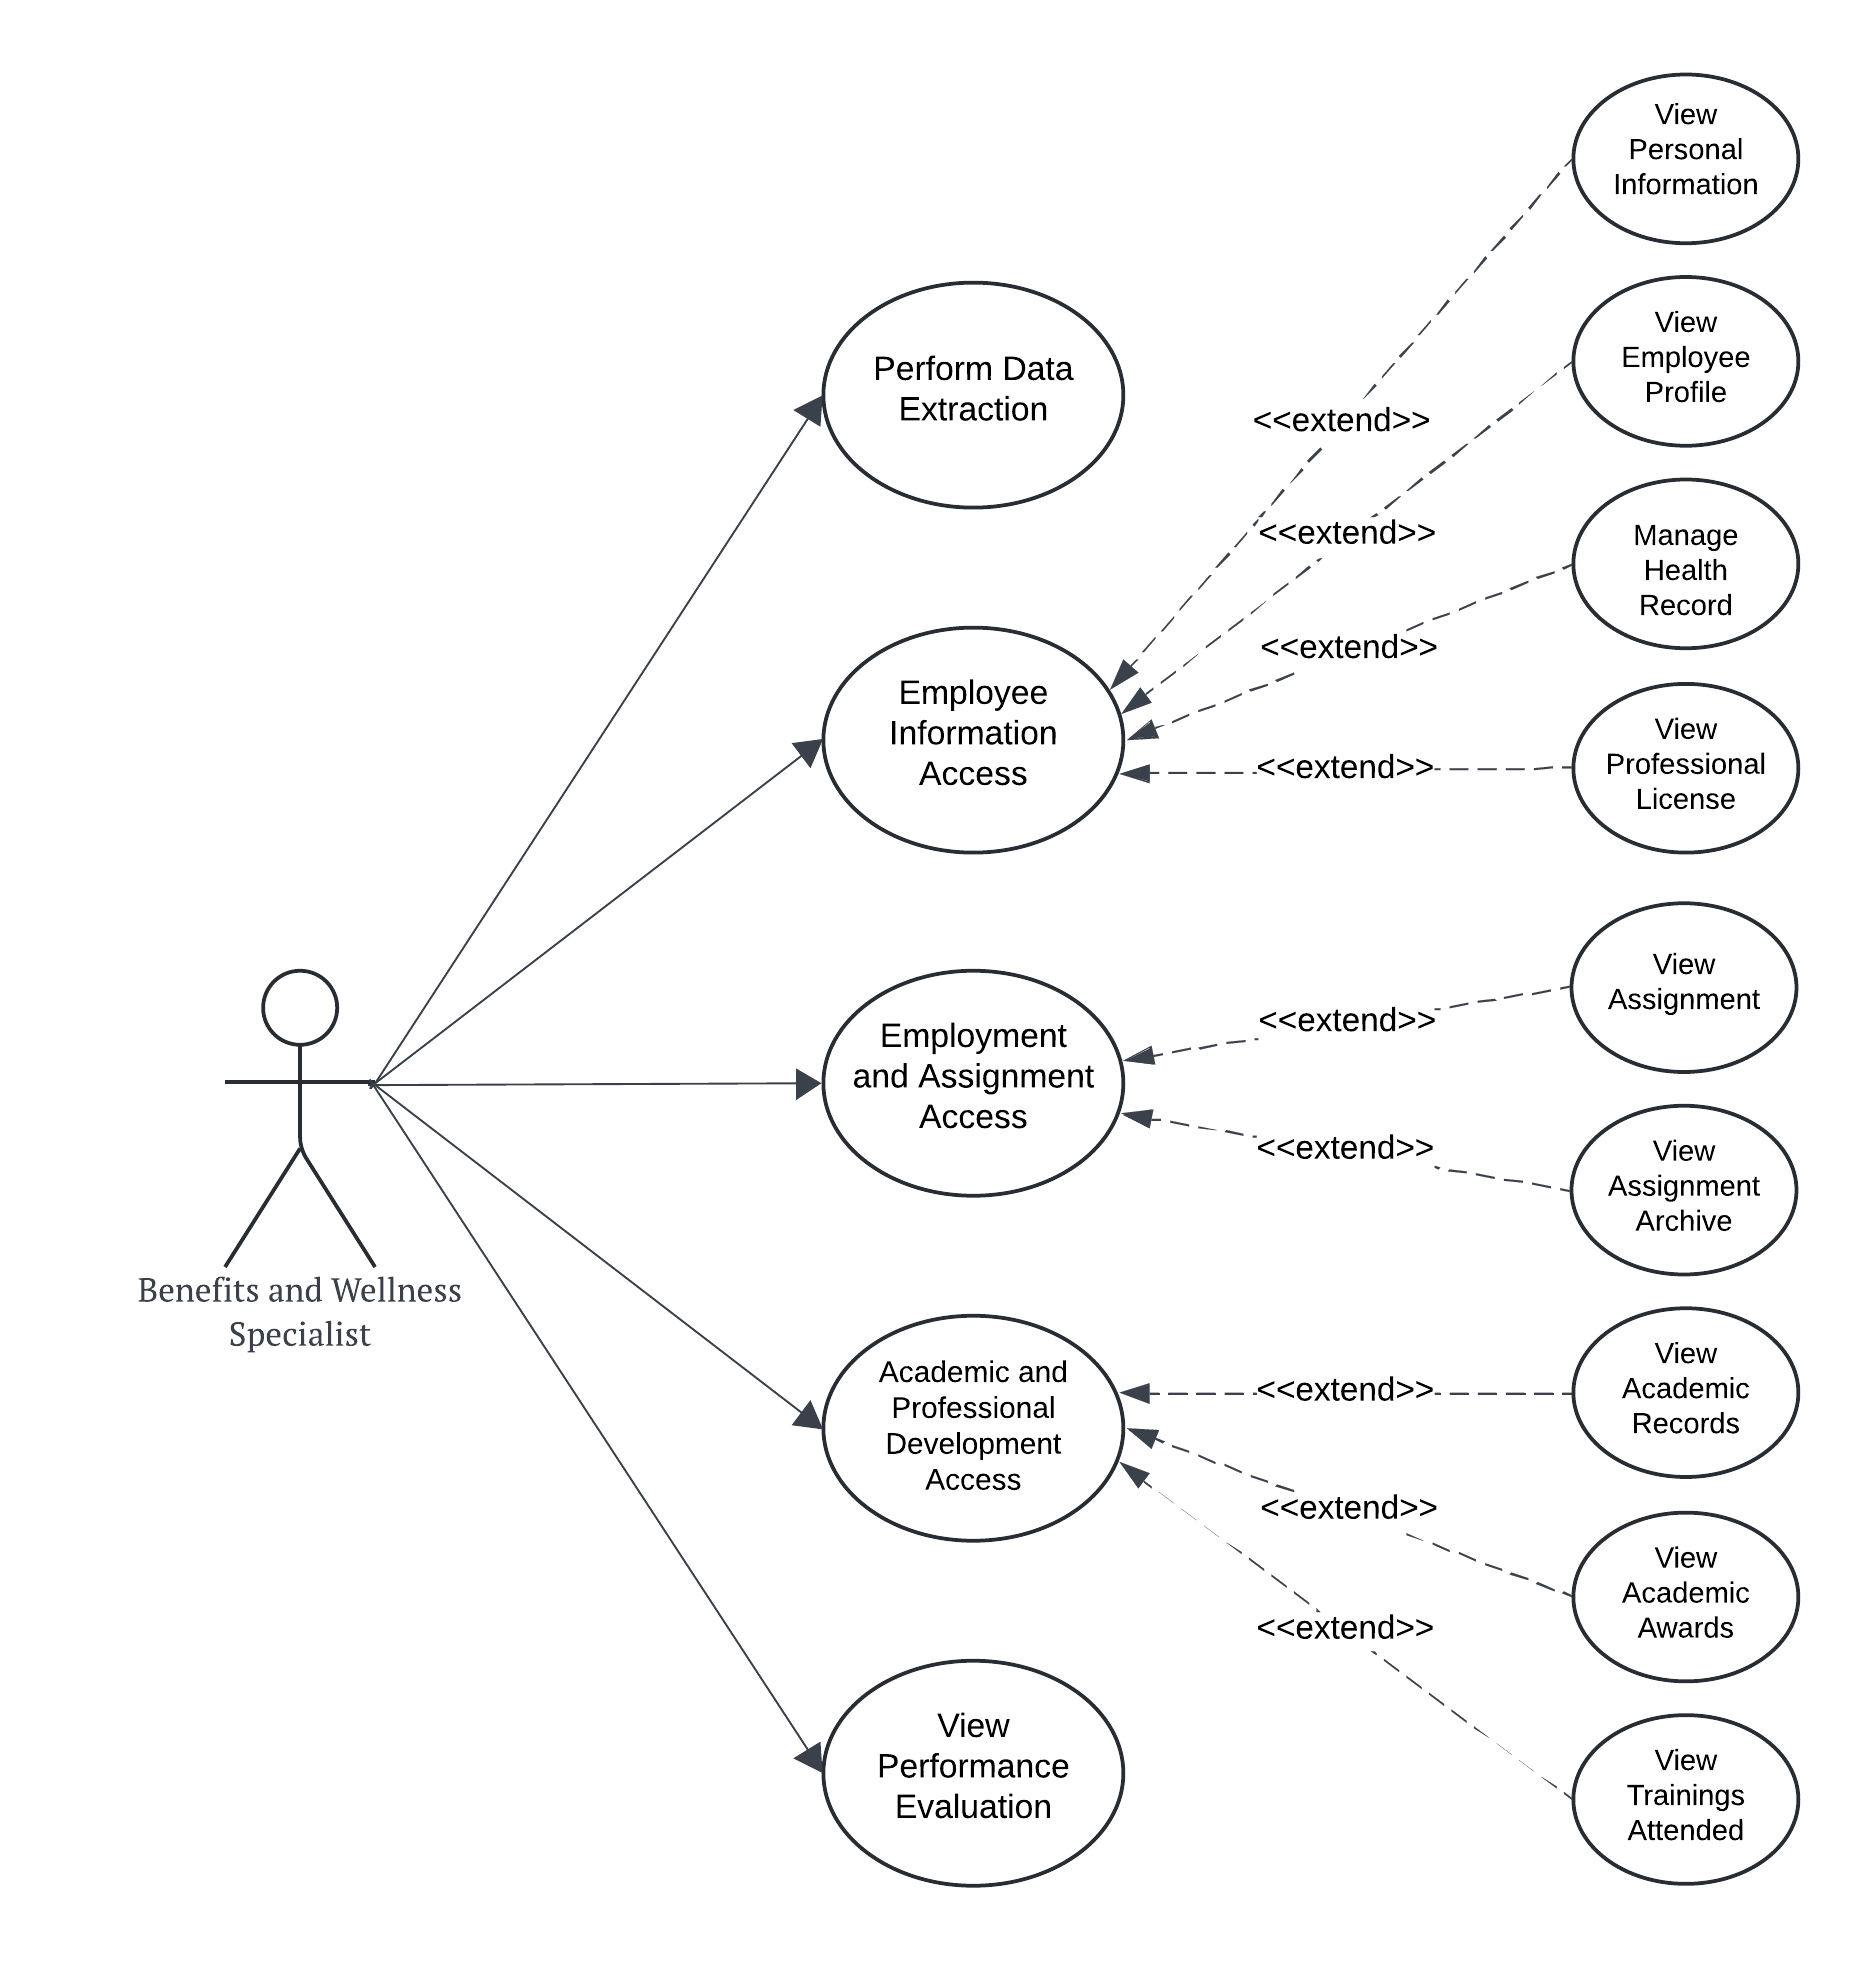
\includegraphics[width=0.9\linewidth]{figures/images/diagrams/usecase/use-case-basic-6.png}
        \caption{HRIS Basic Modules Use Case Diagram: Benefits and Wellness Specialist.}
        \label{fig:use-case-basic-6}
    \end{figure}

    The figure \ref{fig:use-case-basic-6} shows the use case diagram for Benefits and Wellness Specialist. The actor has limited view access to the most of the use cases within the HRIS Basic Modules. This includes Performing Data Extraction, Viewing Performance Evaluation, and also the use cases that  encompasses the 3 functional areas: Employee Information Access, Employment and Assignment Access, and Academic and Professional Development Access. The only exception is that, the Benefits and Wellness Specialist was able to Manage the Health Records of the employees which is found in the Employee Information Access functional area.

    \begin{figure}[H]
        \centering
        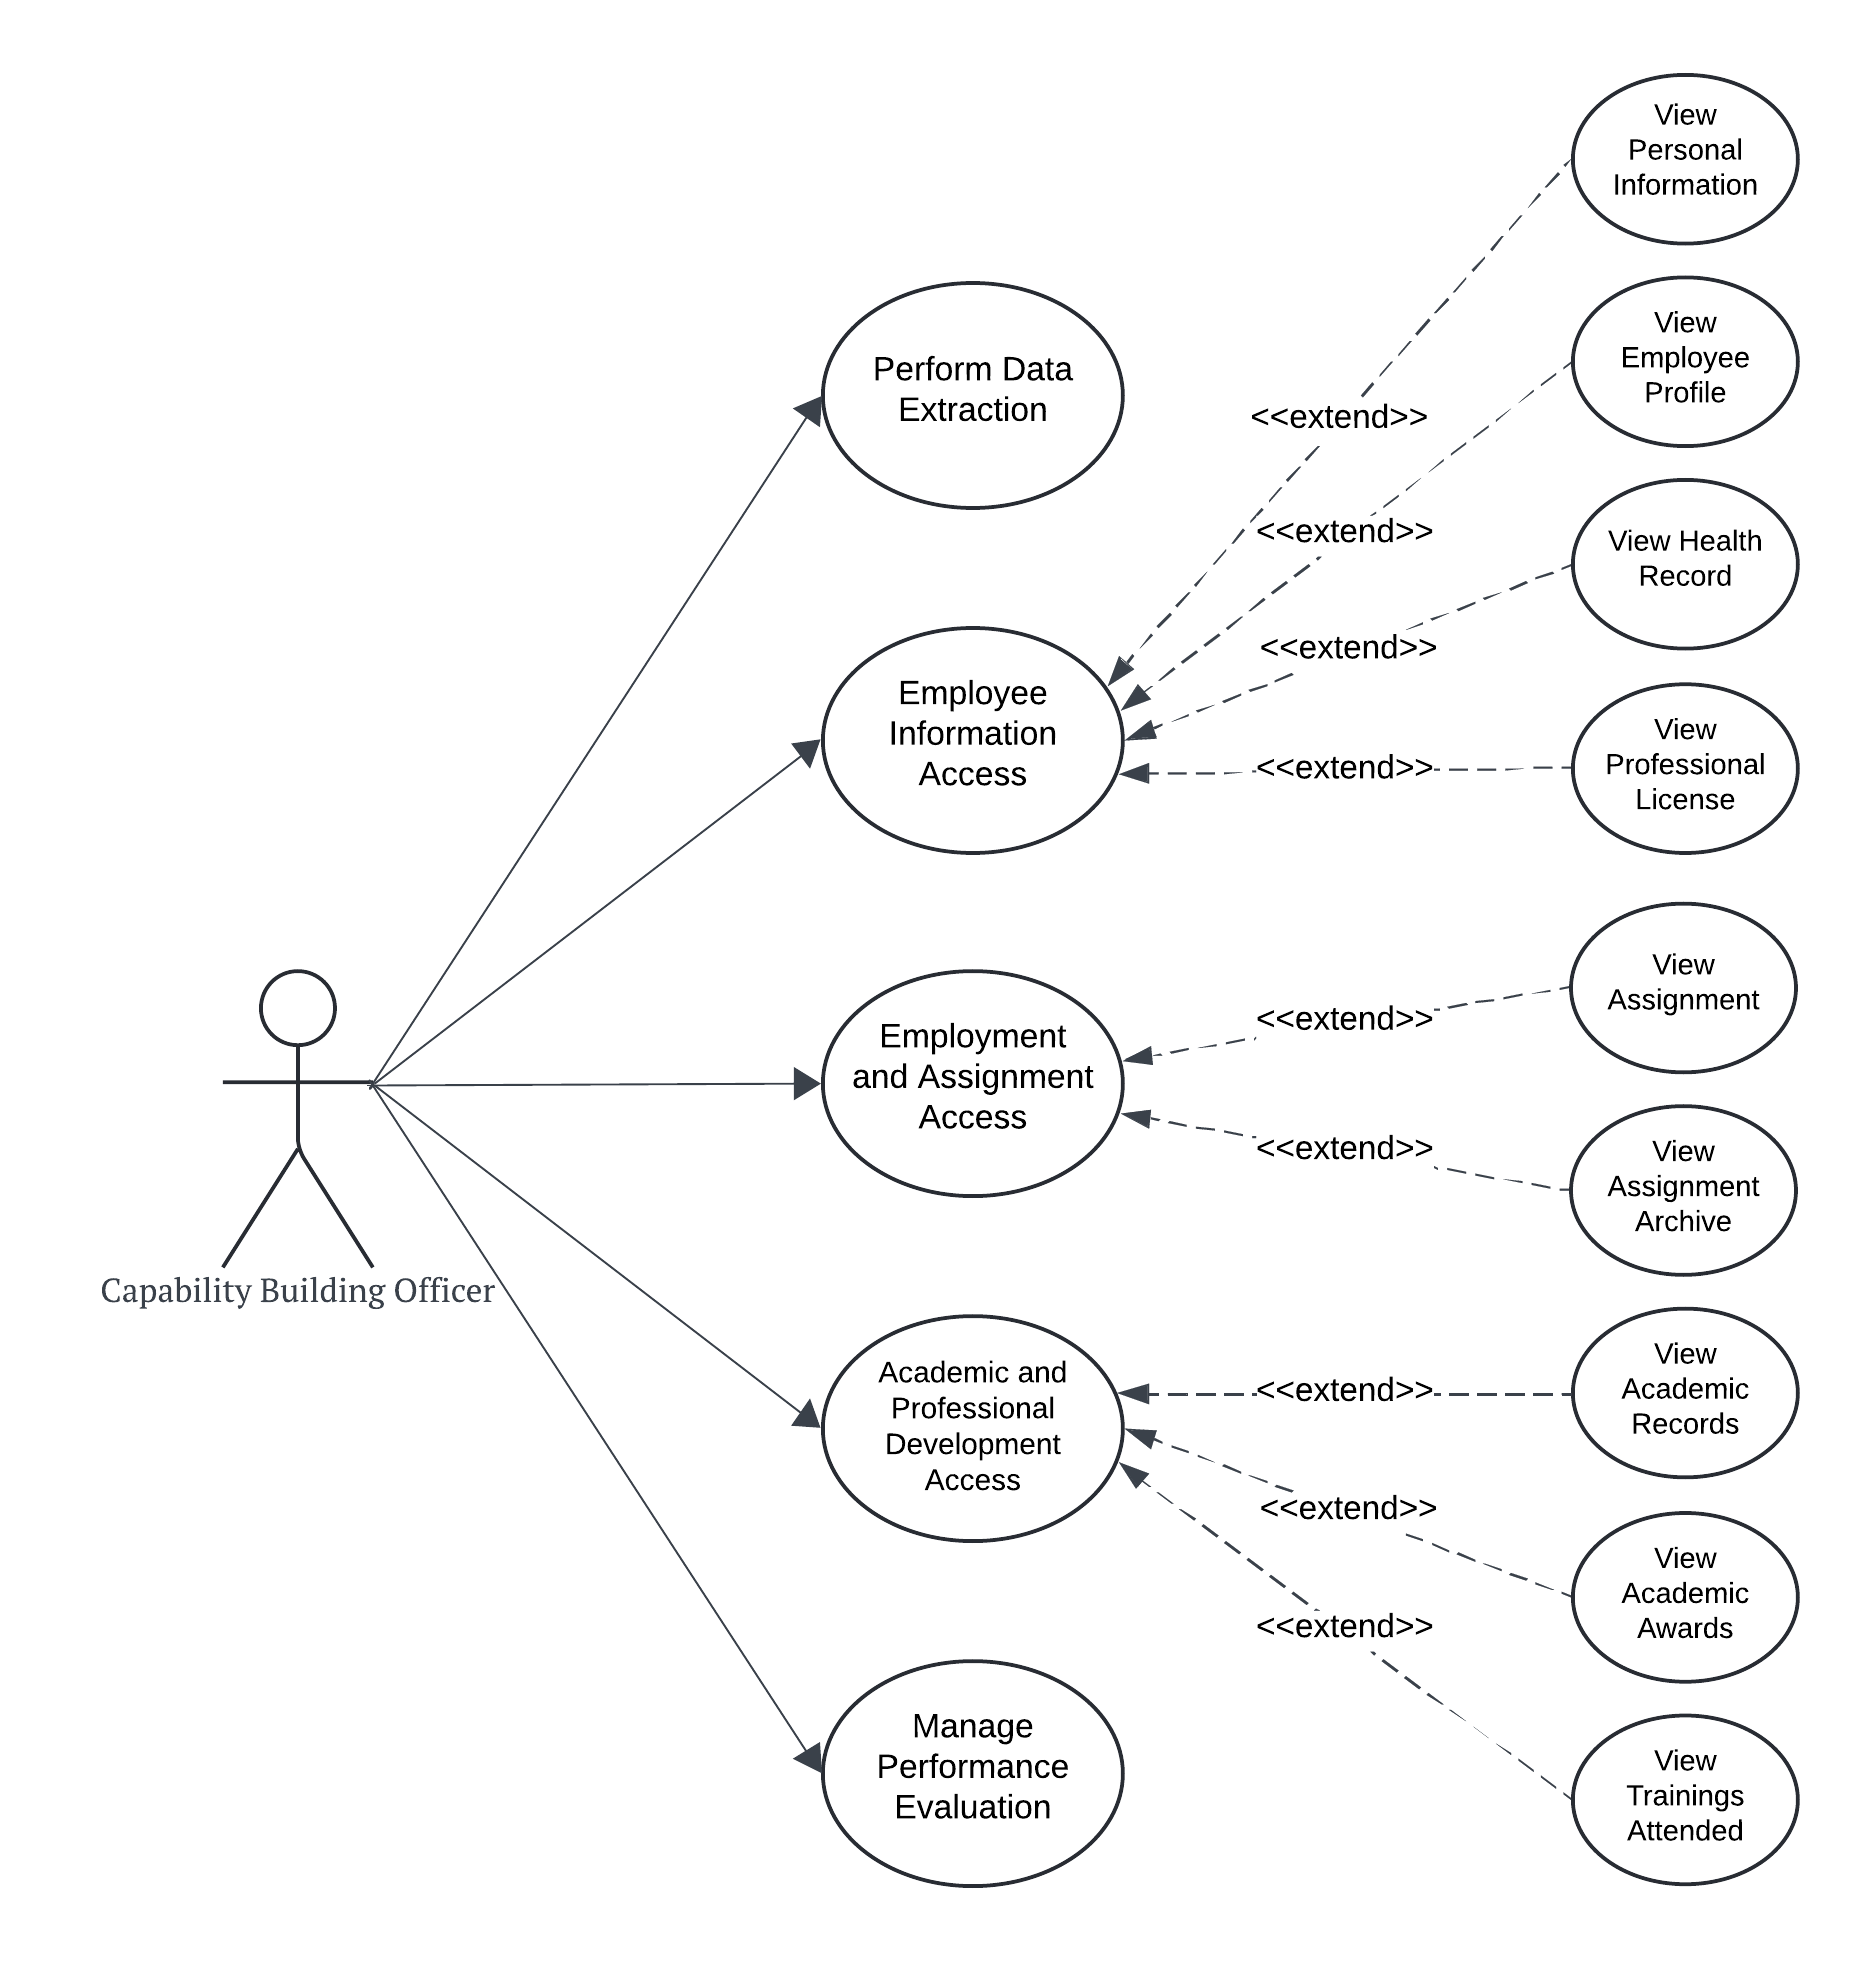
\includegraphics[width=0.9\linewidth]{figures/images/diagrams/usecase/use-case-basic-7.png}
        \caption{HRIS Basic Modules Use Case Diagram: Capability Building Officer.}
        \label{fig:use-case-basic-7}
    \end{figure}

    The figure \ref{fig:use-case-basic-7} illustrates the use case diagram for the Capability Building Officer. The actor has limited view access to the most of the use cases within the HRIS Basic Modules. This includes Performing Data Extraction, and the use cases that  encompasses the 3 functional areas: Employee Information Access, Employment and Assignment Access, and Academic and Professional Development Access. Moreover, the Capability Building Officer has the privilege to Manage the Performance Evaluation of the employees.

    \begin{figure}[H]
        \centering
        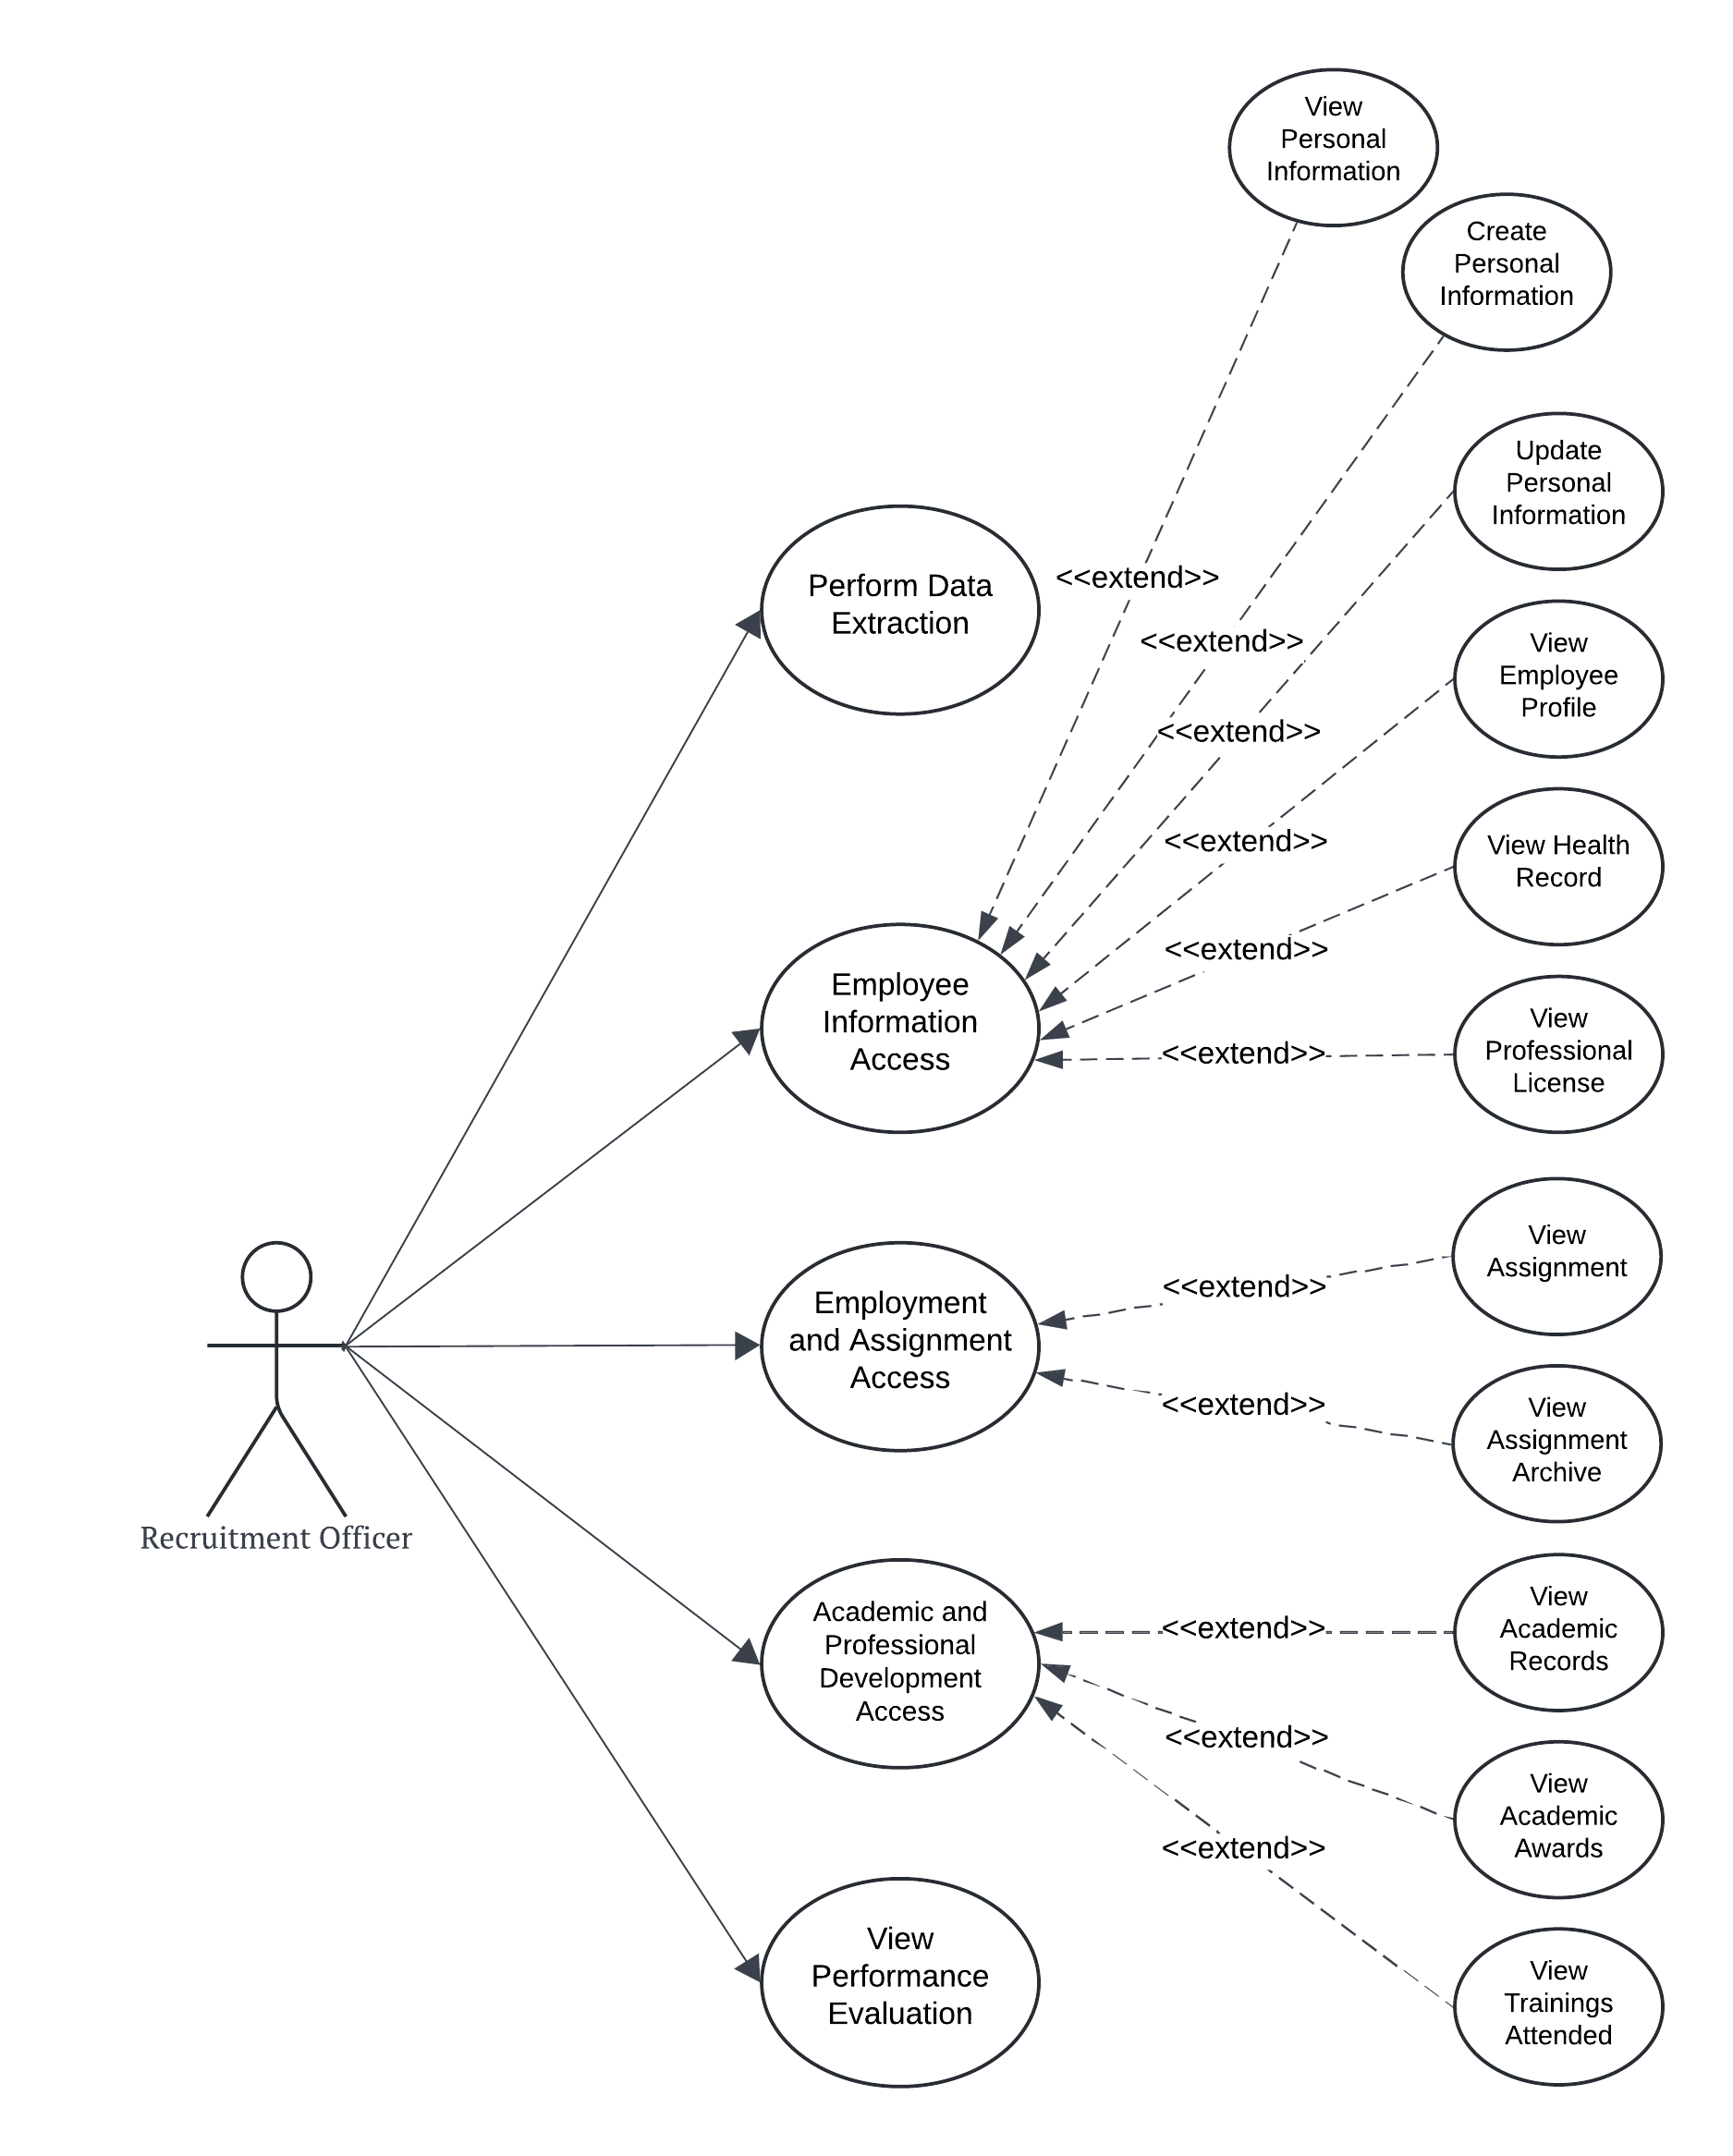
\includegraphics[width=0.9\linewidth]{figures/images/diagrams/usecase/use-case-basic-8.png}
        \caption{HRIS Basic Modules Use Case Diagram: Recruitment Officer.}
        \label{fig:use-case-basic-8}
    \end{figure}

    The figure \ref{fig:use-case-basic-8} illustrates the use case diagram for Recruitment Officers. The actor has limited view access to the most of the use cases within the HRIS Basic Modules. This includes Performing Data Extraction, Viewing Performance Evaluation, and the use cases that  encompasses the 3 functional areas: Employee Information Access, Employment and Assignment Access, and Academic and Professional Development Access. The only exception is that,  in the Employee Information Access functional area, the Recruitment Officer has a distinct privilege which is to view, create, and update the personal information of the employees.


    This section presents the use case diagram for the HRIS TIMESYS Module. The module involves four primary actors: System Admin, Attendance Monitoring Staff, College Faculty Attendance Checker, and Compensation and Benefits Officer. Each actor has specific access to various use cases within the TIMESYS module, enabling them to perform functions related to employee attendance monitoring and management.

    The module encompasses several key use cases, including managing employee attendance. This extends to archived attendance records and the generation of attendance reports. Additionally, it covers use cases related to managing work schedules, overtime, and holidays. A distinct functional area is created specifically for categorizing the management of tardiness, AWOL (Absent Without Leave), and remarks. This structured approach ensures comprehensive coverage of all time-related aspects of employee management.

    This diagram provides a comprehensive overview of the roles and responsibilities within the TIMESYS module, ensuring each actor has the necessary access to perform their tasks effectively.
    
    \begin{figure}[H]
        \centering
        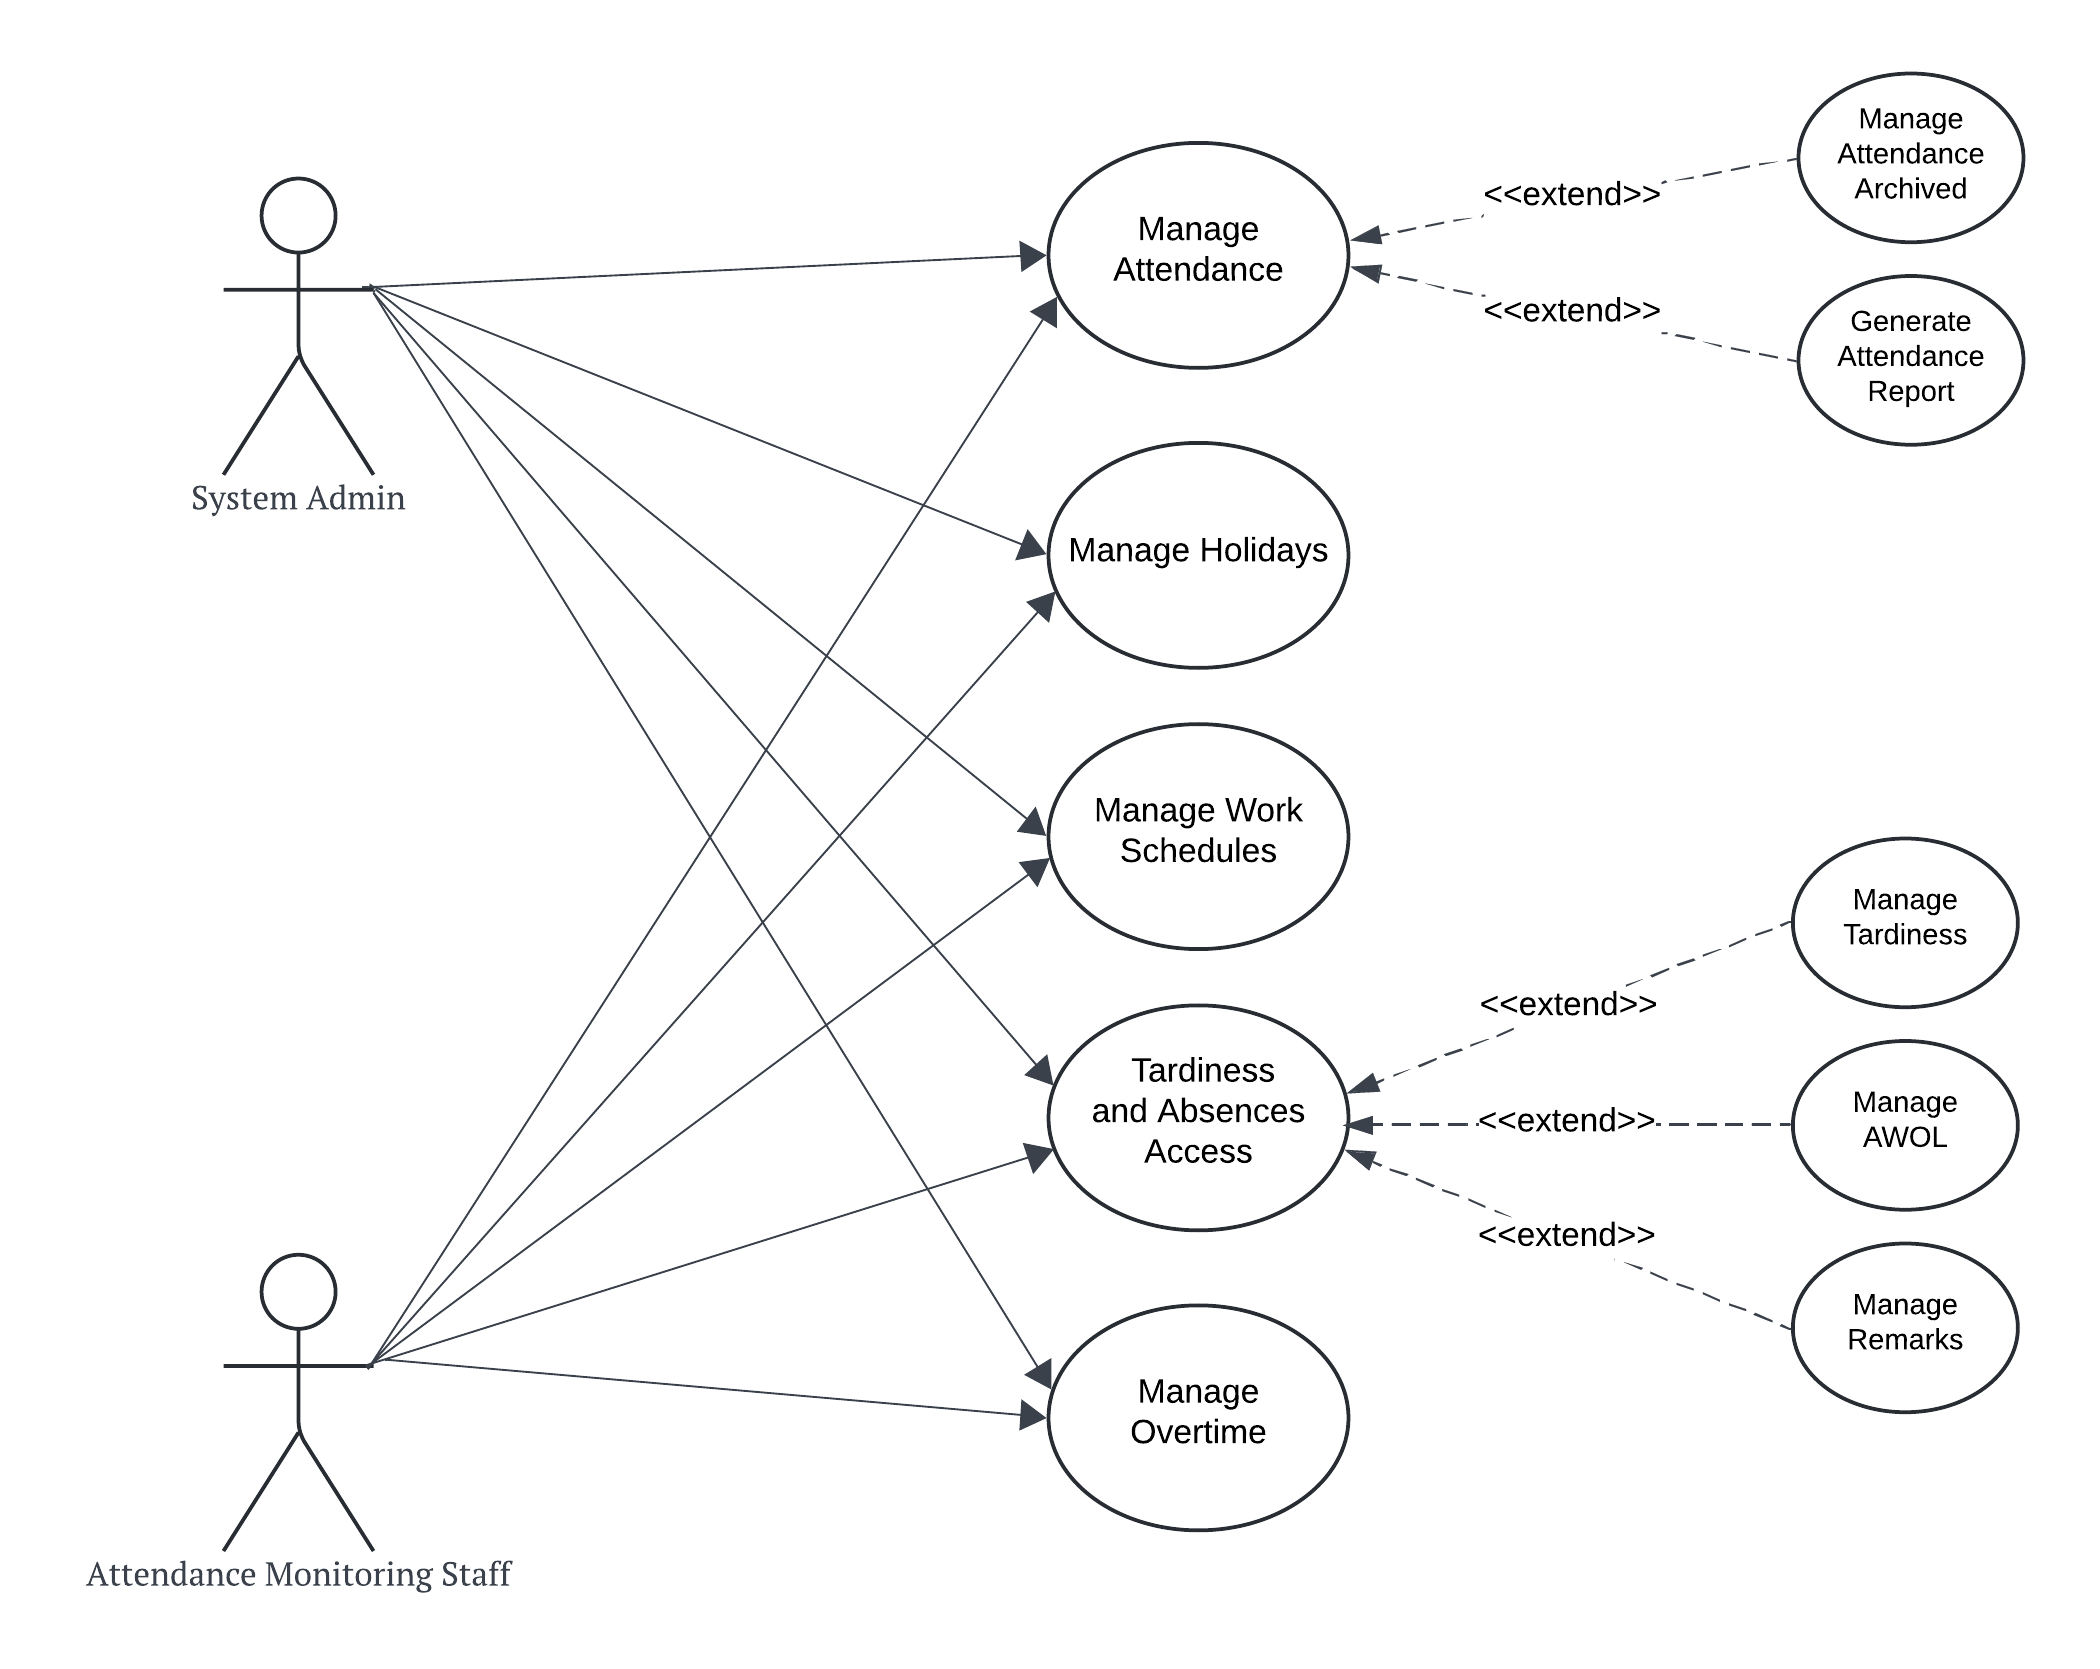
\includegraphics[width=0.9\linewidth]{figures/images/diagrams/usecase/use-case-time-1.png}
        \caption{HRIS TIMESYS Module: System Admin and Attendance Monitoring Staff.}
        \label{fig:use-case-time-1}
    \end{figure}

    The figure \ref{fig:use-case-time-1} demonstrates the use case diagram for the HRIS TIMESYS Module. The diagram shows the use cases for the System Admin and Attendance Monitoring Staff. Both of the actors have full managing access to all use cases found within the TIMESYS module. This comprehensive access enables the System Admin and Attendance Monitoring Staff to oversee and manage all aspects of the TIMESYS module, ensuring efficient and effective attendance monitoring and management.

    \begin{figure}[H]
        \centering
        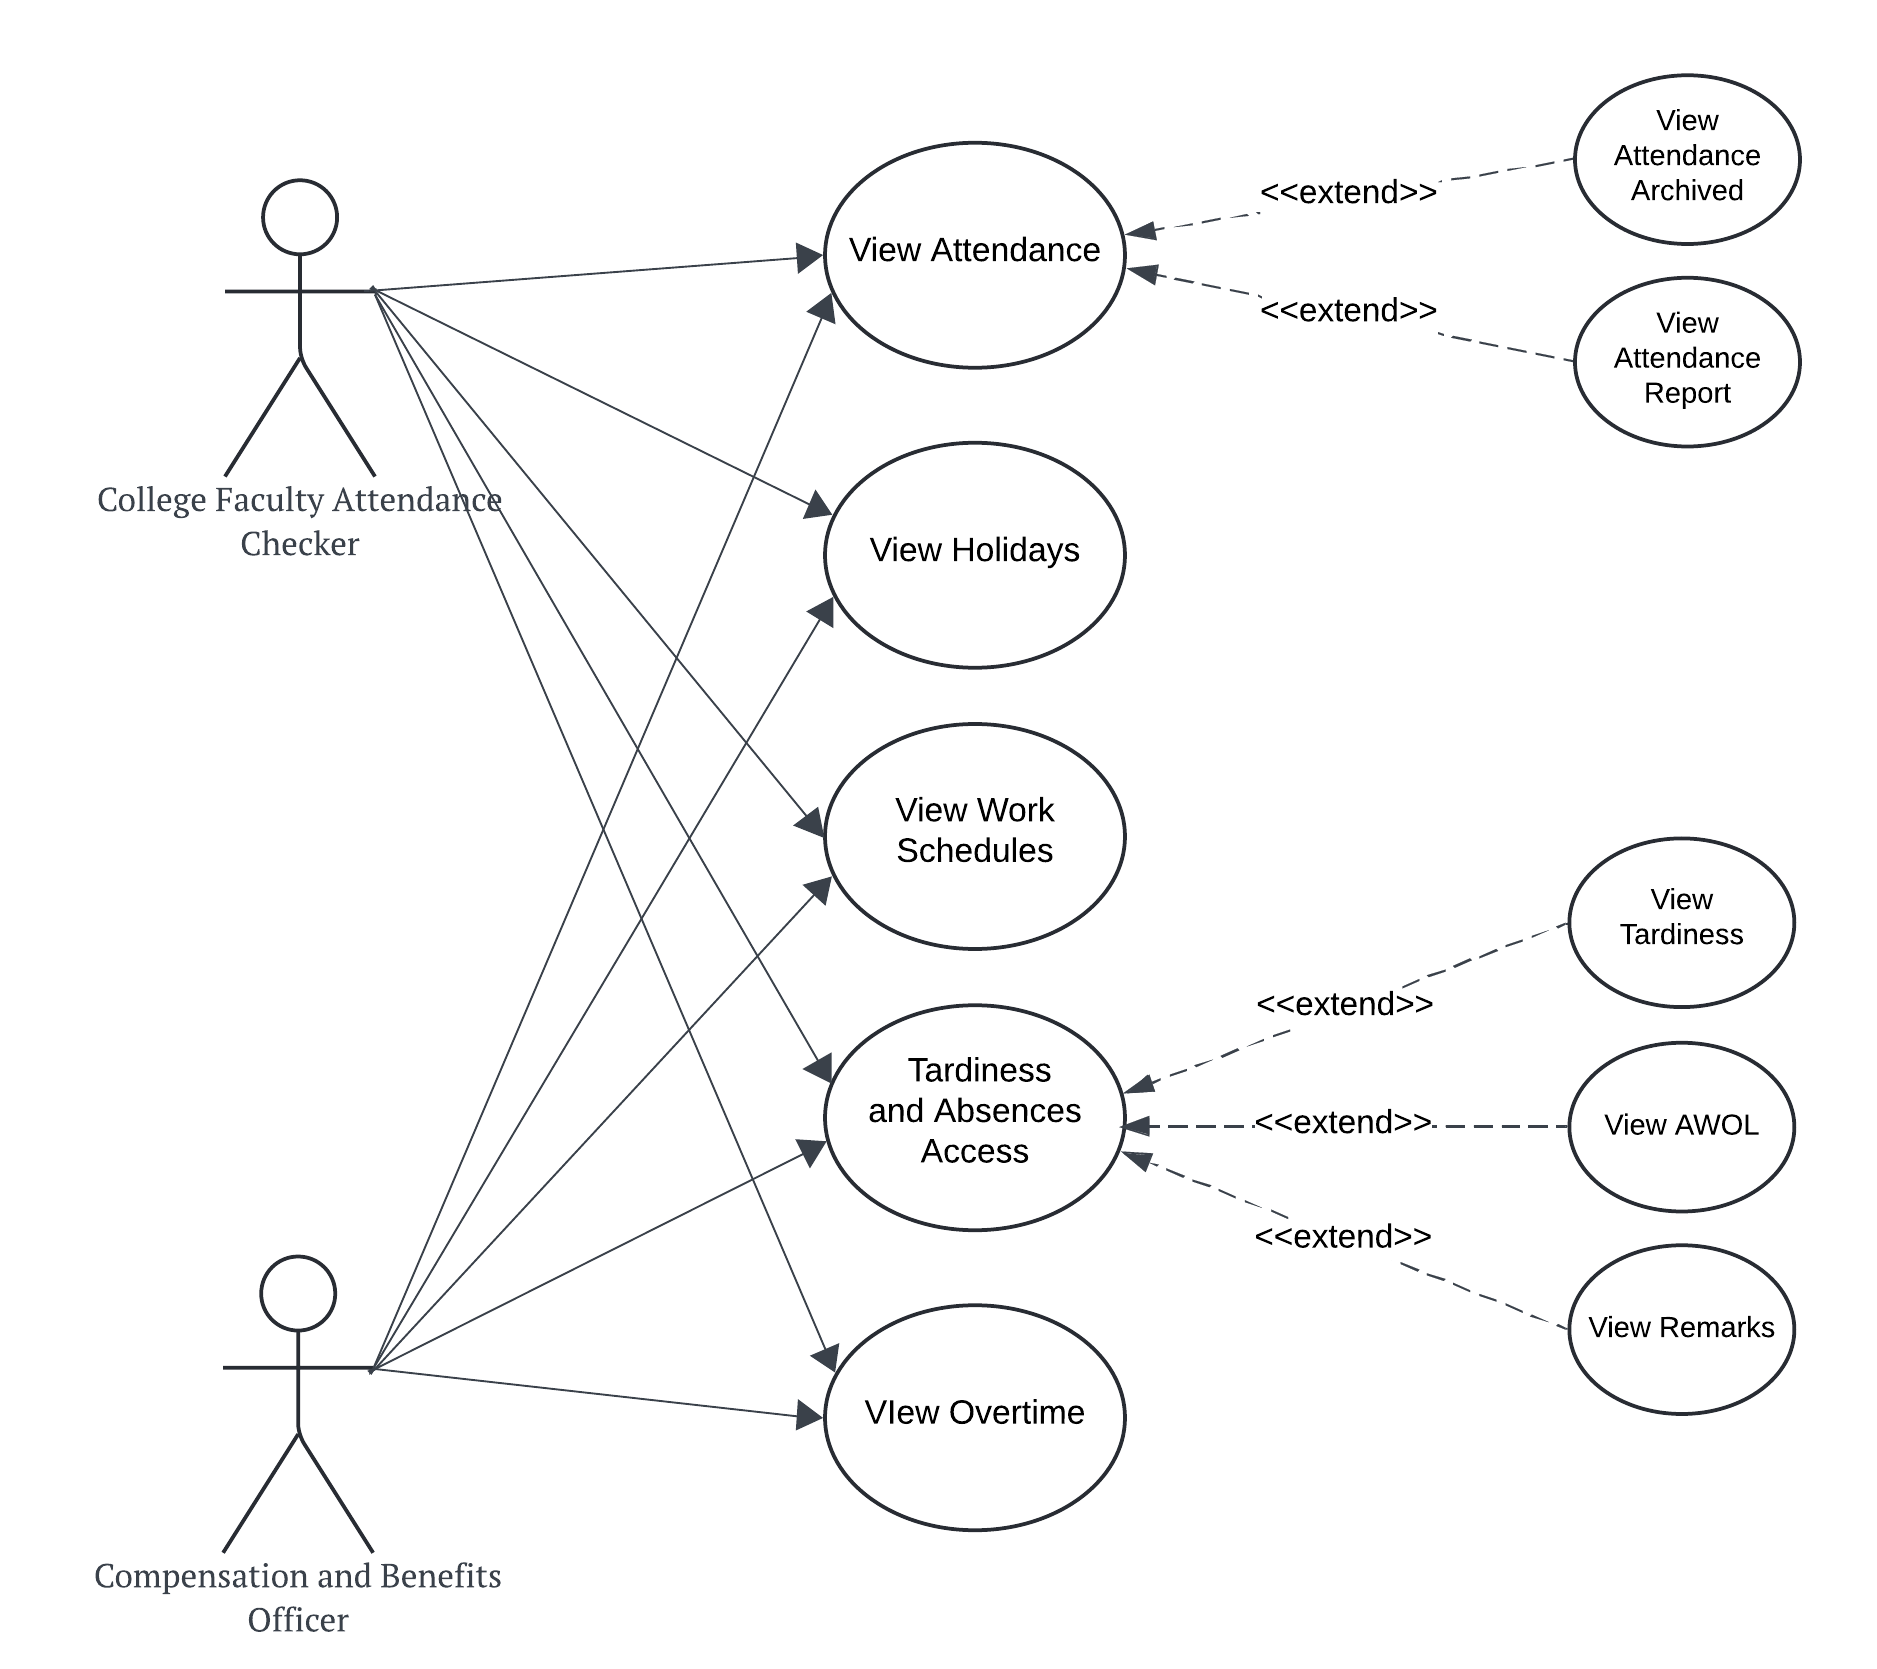
\includegraphics[width=0.9\linewidth]{figures/images/diagrams/usecase/use-case-time-2.png}
        \caption{HRIS TIMESYS Module: College Faculty Attendance Checker and Compensation and Benefits Officer.}
        \label{fig:use-case-time-2}
    \end{figure}

    The figure \ref{fig:use-case-time-2} depicts the use case diagram for the HRIS TIMESYS Module. The diagram illustrates the use cases for the College Faculty Attendance Checker and Compensation and Benefits Officer. Both actors share the same access which is limited to view-only access to all use cases found within the TIMESYS module. 


    In this section, it presents the use case diagrams for the HRIS FACSYS Module. The module involves five primary actors: System Admin, Attendance Monitoring Staff, College Faculty Attendance Checker, Compensation and Benefits Officer, and Student Assistant Attendance Checker. Each actor has specific access to various use cases within the FACSYS module, enabling them to perform functions related to faculty attendance monitoring and management. The FACSYS module consists of three primary use cases: Managing Faculty Attendance, which extends to the generation of faculty attendance reports; Managing Faculty Schedule, which includes handling pending faculty schedules; and Managing Required Class Hours. This structure ensures comprehensive coverage of all faculty attendance-related aspects of employee management.

    \begin{figure}[H]
        \centering
        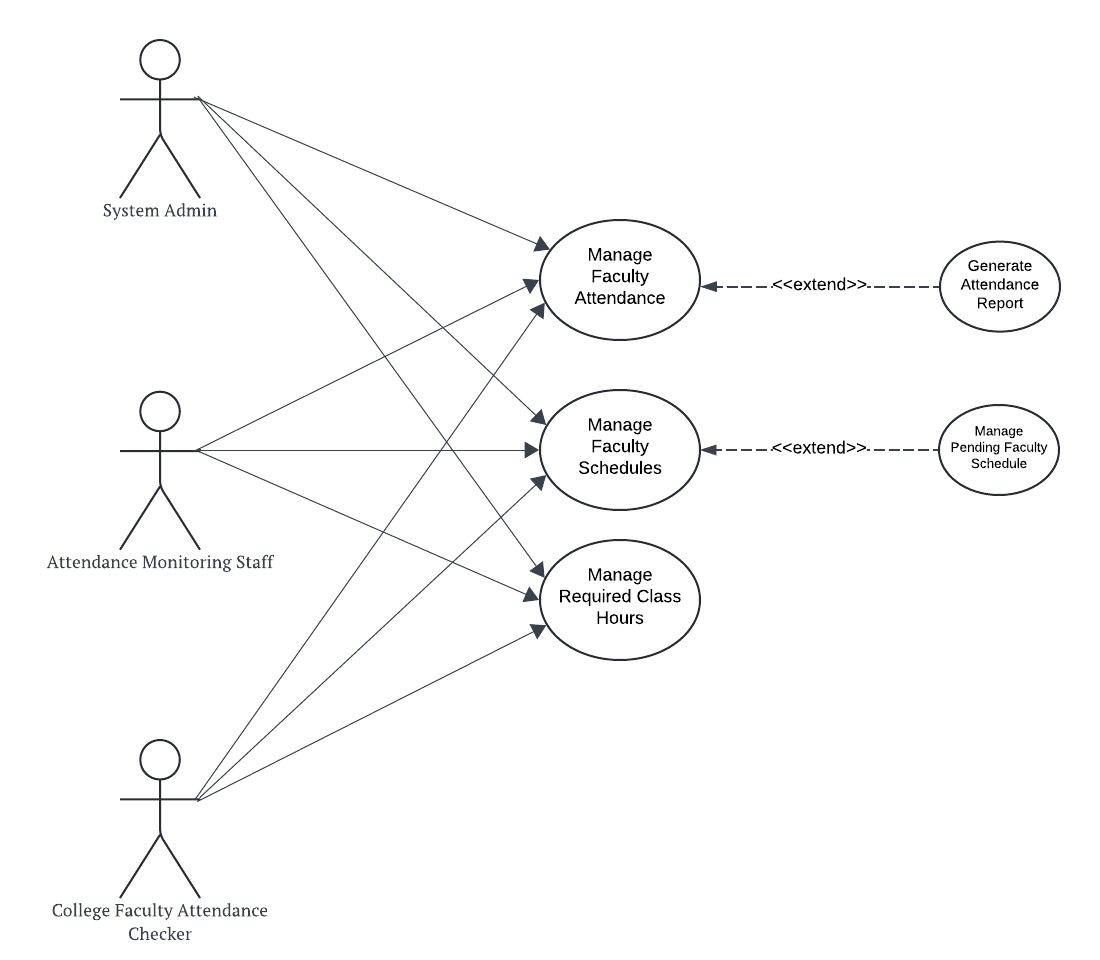
\includegraphics[width=0.9\linewidth]{figures/images/diagrams/usecase/use-case-fac-1.png}
        \caption{HRIS FACSYS Module: System Admin, Attendance Monitoring Staff, and College Faculty Attendance Checker.}
        \label{fig:use-case-fac-1}
    \end{figure}

    The figure \ref{fig:use-case-fac-1} illustrates the use case diagram of the System Admin, Attendance Monitoring Staff, and College Faculty Attendance Checker within the HRIS FACSYS Module. These three actors share the same full managing access to all use cases found within the FACSYS module. This comprehensive access enables the System Admin, Attendance Monitoring Staff, and College Faculty Attendance Checker to oversee and manage all aspects of the FACSYS module, ensuring efficient and effective faculty attendance monitoring and management.

    \begin{figure}[H]
        \centering
        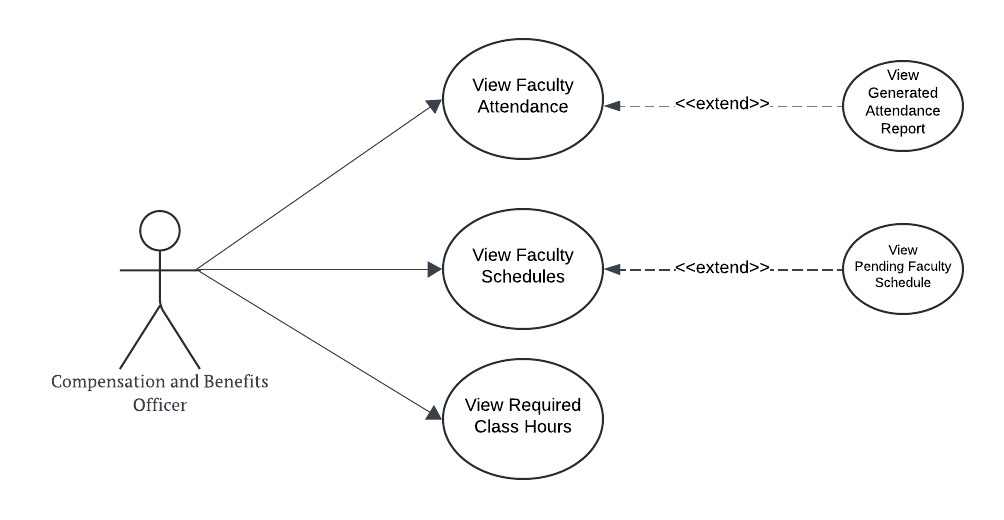
\includegraphics[width=0.9\linewidth]{figures/images/diagrams/usecase/use-case-fac-2.png}
        \caption{HRIS FACSYS Module: Compensation and Benefits Officer.}
        \label{fig:use-case-fac-2}
    \end{figure}

    The figure \ref{fig:use-case-fac-2} shows the use case diagram for the Compensation and Benefits Officer. The actor has limited view access to all of the use cases found within the FACSYS module. This includes Viewing Faculty Attendance, which extends to viewing of generated faculty attendance report; Viewing Faculty Schedule, which includes viewing of pending faculty schedules; and Viewing Required Class Hours. This structure ensures that the Compensation and Benefits Officer has the necessary access to view faculty attendance and schedule information, facilitating efficient monitoring and management of faculty attendance.

    \begin{figure}[H]
        \centering
        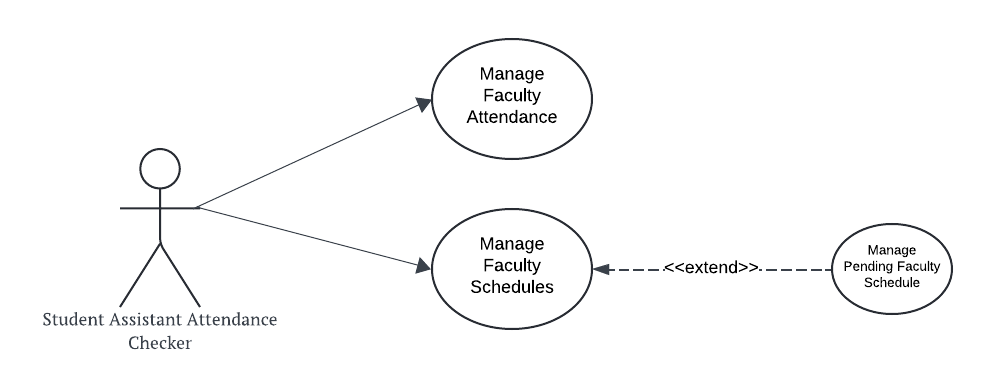
\includegraphics[width=0.9\linewidth]{figures/images/diagrams/usecase/use-case-fac-3.png}
        \caption{HRIS FACSYS Module: Student Asssitant Attendance Checker.}
        \label{fig:use-case-fac-3}
    \end{figure}

    The figure \ref{fig:use-case-fac-3} illustrates the use case diagram for the Student Assistant Attendance Checker. The actor has limited manage access to the use cases found within the FACSYS module. The Student Assistant Attendance Checker has the privilege to manage faculty attendance but wasn't able to generate faculty attendance report, and manage faculty schedule as well as managing the pending faculty schedules. This structure ensures that the Student Assistant Attendance Checker has the necessary access to manage faculty attendance, facilitating efficient monitoring and management of faculty attendance. 
    

    This section presents the use case diagrams for the HRIS LEAVESYS Module. The module involves four primary actors: System Admin, Attendance Monitoring Staff, College Faculty Attendance Checker, and Compensation and Benefits Officer. Each actor has specific access to various use cases within the LEAVESYS module, enabling them to perform functions related to employee leave management and processing. The LEAVESYS module consists of two primary use cases: Managing Leave Applications and Managing Leave Credits. The Managing Leave Applications use case extends to the management of leave reasons, while both Managing Leave Applications and Managing Leave Credits extend to the generation of leave application with Credits Report. This structure allows for comprehensive leave management, encompassing application processing, credit tracking, and reporting functionalities.

    \begin{figure}[H]
        \centering
        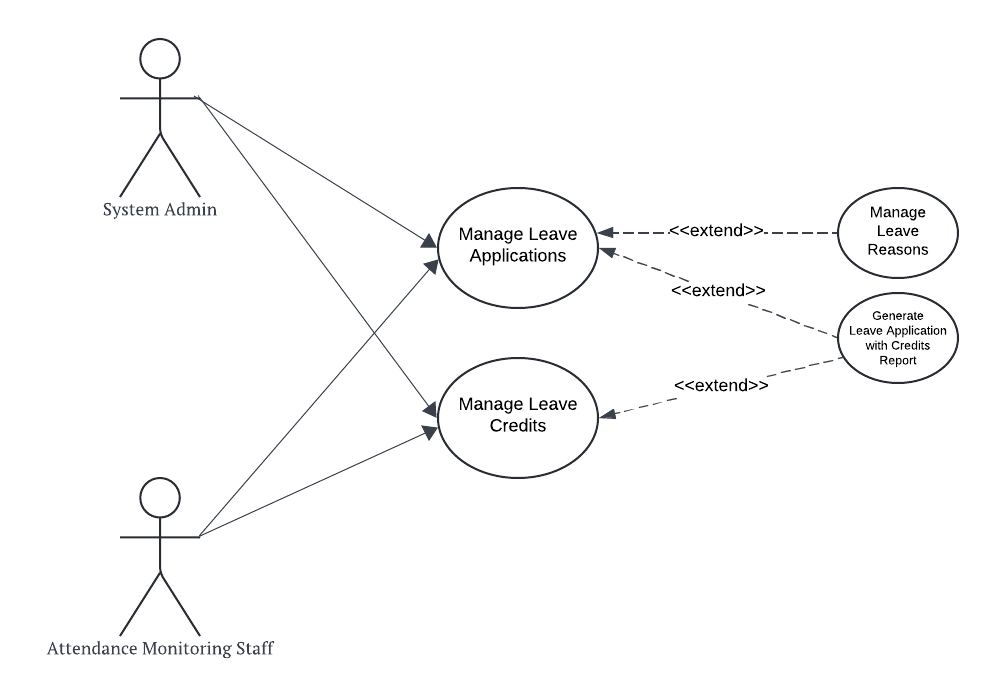
\includegraphics[width=0.9\linewidth]{figures/images/diagrams/usecase/use-case-leave-1.png}
        \caption{HRIS LEAVESYS Module: System Admin and Attendance Monitoring Staff.}
        \label{fig:use-case-leave-1}
    \end{figure}

    Figure \ref{fig:use-case-leave-1} illustrates the use case diagram for the System Admin and Attendance Monitoring Staff within the HRIS LEAVESYS Module. Both actors share full management access to all use cases within the LEAVESYS module. This includes Managing Leave Applications, which extends to managing leave reasons; and Managing Leave Credits. Both of the actors are able to Generate Leave Application with Credits Report. This comprehensive access enables the System Admin and Attendance Monitoring Staff to oversee and manage all aspects of the LEAVESYS module, ensuring efficient and effective leave management and processing.

    \begin{figure}[H]
        \centering
        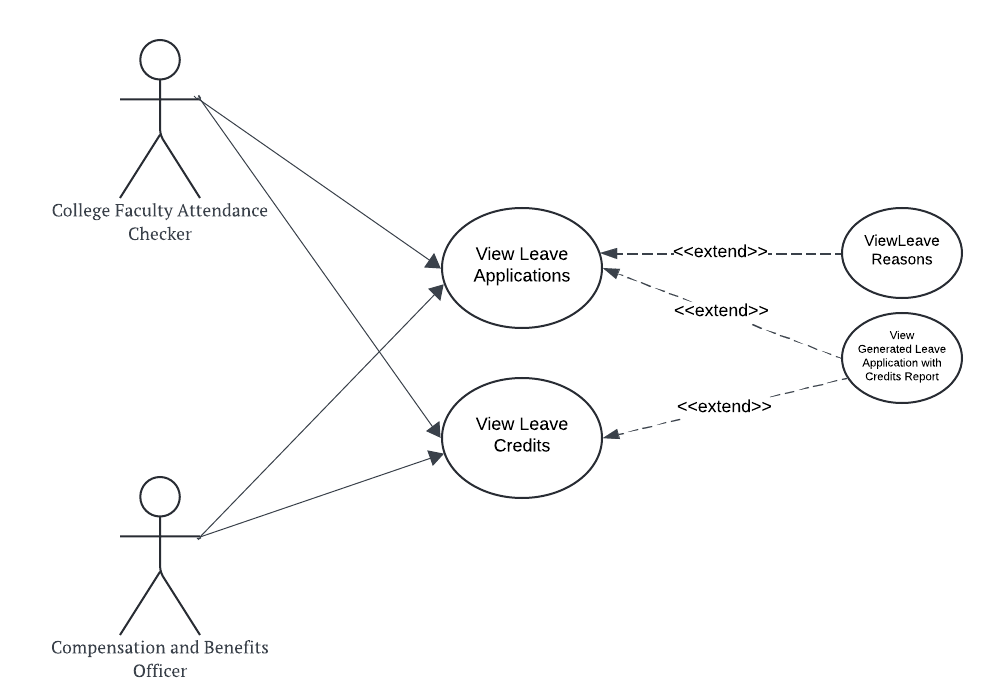
\includegraphics[width=0.9\linewidth]{figures/images/diagrams/usecase/use-case-leave-2.png}
        \caption{HRIS LEAVESYS Module: College Faculty Attendance Checker and Compensation and Benefits Officer.}
        \label{fig:use-case-leave-2}
    \end{figure}

    The figure \ref{fig:use-case-leave-2} depicts the use case diagram for the College Faculty Attendance Checker and Compensation and Benefits Officer within the HRIS LEAVESYS Module. Both actors share the same access which is limited to view-only access to all use cases found within the LEAVESYS module. This includes Viewing Leave Applications, which extends to viewing leave reasons; and Viewing Leave Credits. Both of the actors are only limited to viewing the Generated Leave Application with Credits Report. This structure ensures that the College Faculty Attendance Checker and Compensation and Benefits Officer have the necessary access to view leave applications, credits, and reports, facilitating efficient leave management and processing.


    \subsection{Entity Relational Diagram}
    
    The Entity Relational Diagram (ERD) will be used to visually represent the database structure that defines the relationships between different entities in the system and how they are related to one another through cardinalities and relationships. In the case of the HRIS application, MIS has provided ready access to the database scheme in preparation for the migration process. This ERD represents the various entities such as employees, departments, positions, and their relationships with each other. 
    
    Creating an ERD will allow the developers to design a database schema that accurately represents the data requirements of the HRIS system. This diagram is not only crucial for ensuring data integrity, normalization, and efficient data retrieval, but will also standardize and comply with the DBA requirements of the MIS for merge request and reviewing processes.

    \begin{figure}[H]
        \centering
        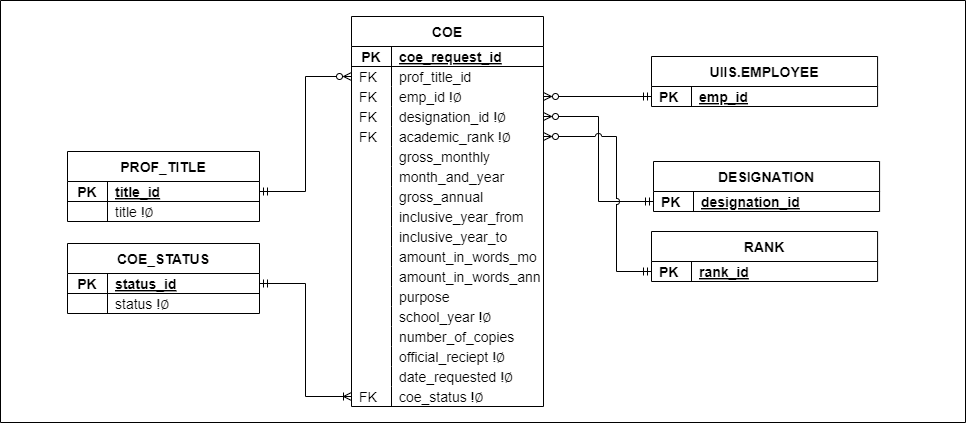
\includegraphics[width=1\linewidth]{figures/images/diagrams/erd/erd-core-coe.png}
        \caption{HRIS Core: Certificate of Employment ERD Model.}
        \label{fig:erd-core-coe} 
    \end{figure}

    This segment of the ERD model illustrates the Certificate of Employment (COE) module within the Human Resource Information System. The system is designed to efficiently manage and generate Certificates of Employment, incorporating various relevant factors for comprehensive employee documentation. Central to this module is the \texttt{hr.coe} entity, which is intricately connected to several other key entities. It links to \texttt{uiis.employee} for essential employee data, ensuring accurate personal information. The system also incorporates \texttt{hr.prof\_title} for the employee's professional designation, \texttt{hr.coe\_status} to track the current status of each certificate, \texttt{hr.office\_unit} to associate the employee with their specific department, \texttt{hr.designation} to capture the official job title, \texttt{hr.rank} to include information about the employee's hierarchical position, and \texttt{hr.employee\_status} to indicate their current employment arrangement. This structure enables the system to generate comprehensive and accurate Certificates of Employment, pulling relevant information from interconnected entities.

    \begin{figure}[H]
        \centering
        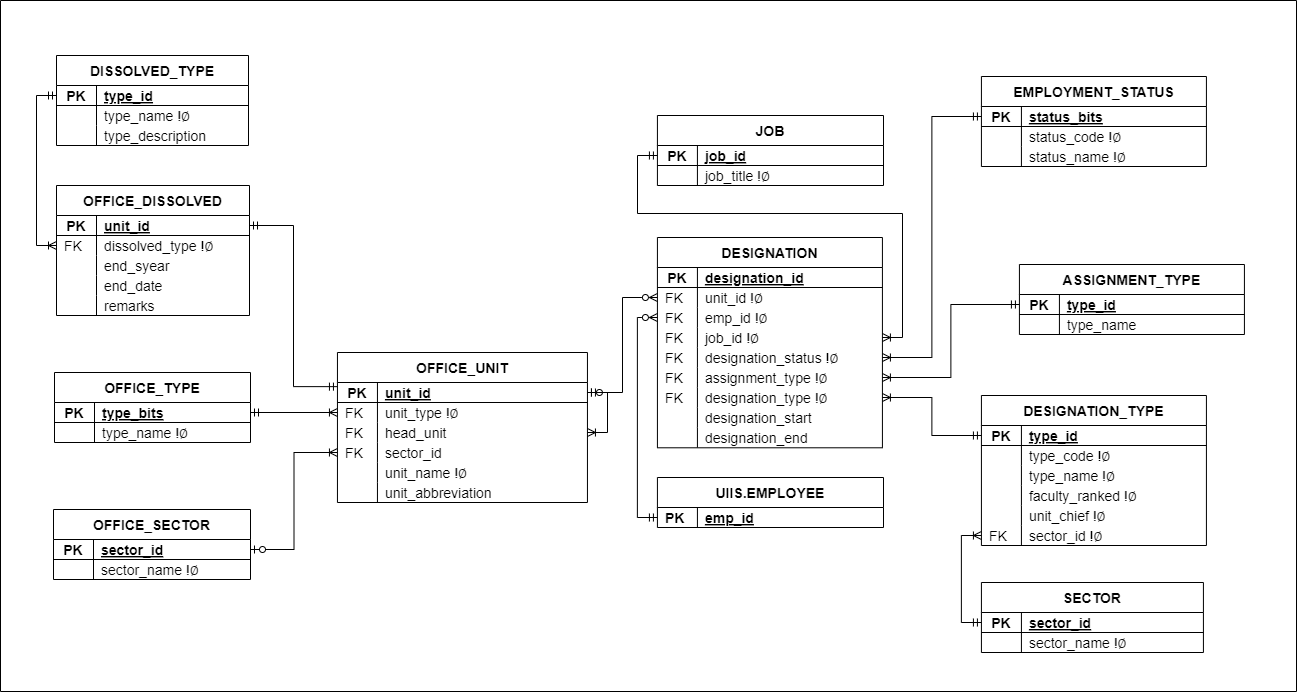
\includegraphics[width=1\linewidth]{figures/images/diagrams/erd/erd-core-office.png}
        \caption{HRIS Core: Designation ERD Model.}
        \label{fig:erd-core-office}
    \end{figure}

    The illutstration shows the ERD model for the designation module which is designed to manage the complex organizational structure and employee positions within the institution. The central \texttt{hr.designation} entity is linked to several other entities, providing a comprehensive view of each employee's position and organizational context. It connects to \texttt{uiis.employee} for individual employee data, \texttt{hr.office\_unit} for departmental information, and \texttt{hr.job} for specific job titles. The system incorporates \texttt{hr.employment\_status} to track the nature of employment (e.g., full-time, part-time), \texttt{hr.assignment\_type} for the kind of role assignment, and \texttt{hr.designation\_type} for categorizing positions. The \texttt{hr.designation\_type} entity further links to \texttt{hr.sector}, allowing for broader organizational grouping. The \texttt{hr.office\_unit} entity is part of a larger organizational structure, connecting to \texttt{hr.office\_sector} and \texttt{hr.office\_type} for detailed unit categorization. It also links to \texttt{hr.office\_dissolved} (which is also connects to \texttt{hr.dissolved\_type}), enabling the system to track historical changes in the organizational structure.

    \begin{figure}[H]
        \centering
        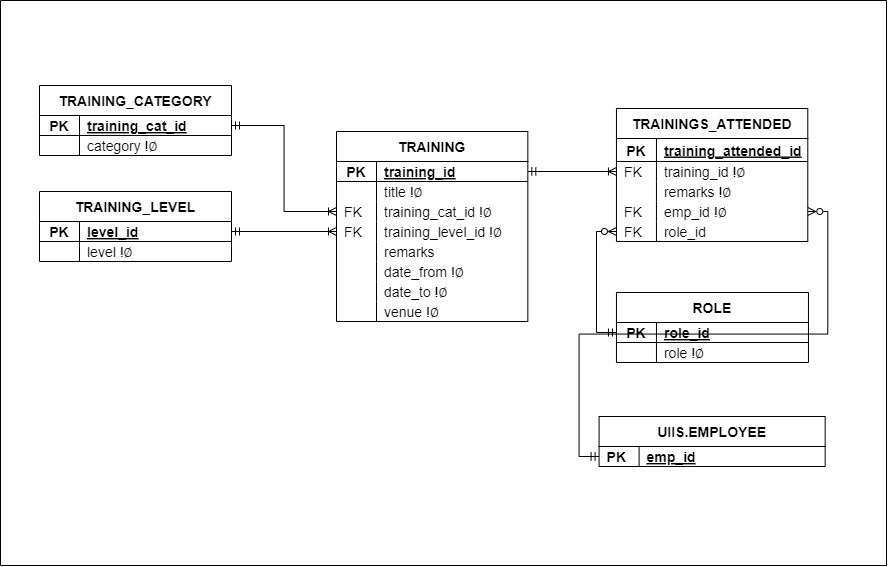
\includegraphics[width=1\linewidth]{figures/images/diagrams/erd/erd-core-trainings.png}
        \caption{HRIS Core: Trainings ERD Model.}
        \label{fig:erd-core-trainings}
    \end{figure}

    This part of the ERD model illustrates the Training module within the Human Resource Information System. The system is designed to comprehensively track and manage employee training activities. The central entity is \texttt{hr.training}, which captures essential details such as training title, date range, venue, and remarks. It's connected to \texttt{hr.training\_category} and \texttt{hr.training\_level}, allowing for classification of training types and levels of complexity or importance. The \texttt{hr.training\_attended} entity serves as a connection between individual employees \texttt{uiis.employee} and specific training sessions, also incorporating the \texttt{hr.role} of the employee in each training. This structure enables detailed recording of each employee's training history, including their role in each session.

    \begin{figure}[H]
        \centering
        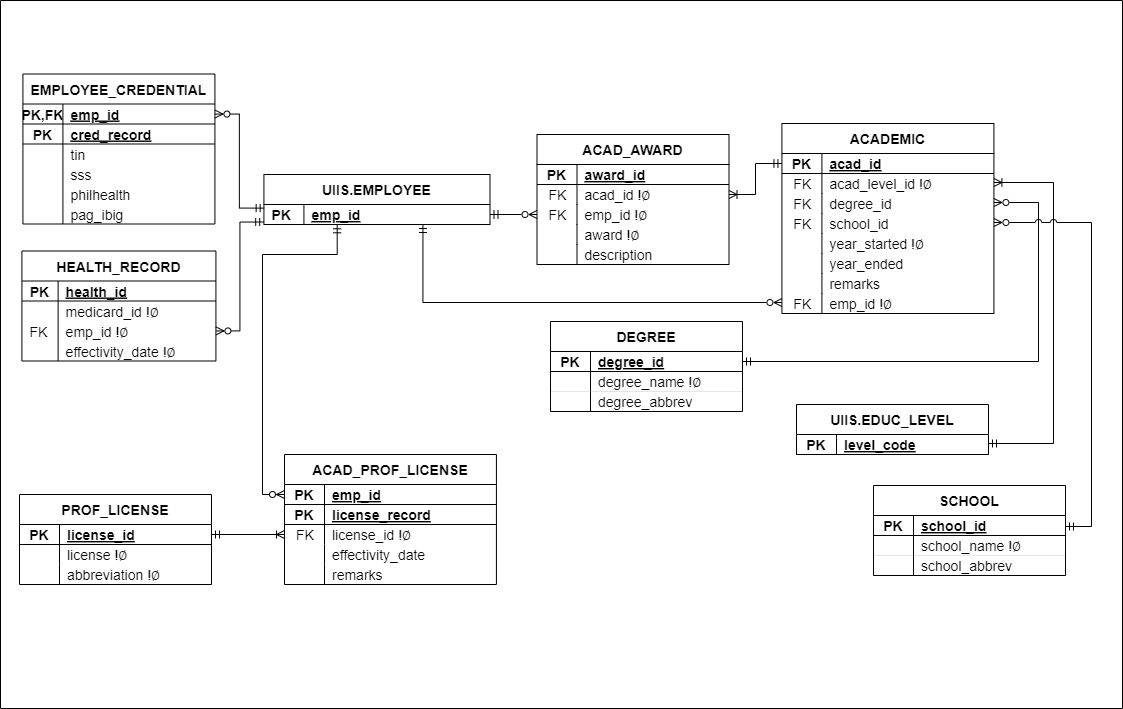
\includegraphics[width=1\linewidth]{figures/images/diagrams/erd/erd-core-emp-personal-info.png}
        \caption{HRIS Core: Employee Personal Information ERD Model.}
        \label{fig:erd-core-emp-personal-info}
    \end{figure}

    This segment of the Human Resource Information System is designed to manage comprehensive personal and professional information for each employee. The system revolves around the \texttt{uiis.employee} entity, which serves as the central point connecting various aspects of an employee's profile. The \texttt{hr.employee\_credential} entity stores essential identification and access information, directly linked to the employee record. Health-related information is captured in the \texttt{hr.health\_record} entity, ensuring that important medical id is securely associated with each employee. The \texttt{hr.academic} entity tracks educational background, connecting not only to the employee but also to \texttt{hr.school}, \texttt{uiis.educ\_level}, and \texttt{hr.degree} entities, allowing for a detailed educational history. 
            
    Academic achievements are recorded in the \texttt{hr.acad\_awards} entity, linked to both the employee and their academic records. Professional qualifications are managed through the \texttt{hr.acad\_prof\_license} entity, which connects employees to their professional licenses. This structure enables a holistic view of each employee's personal, educational, and professional qualifications, supporting various HR functions such as career development, compliance, and employee wellness initiatives.

    \begin{figure}[H]
        \centering
        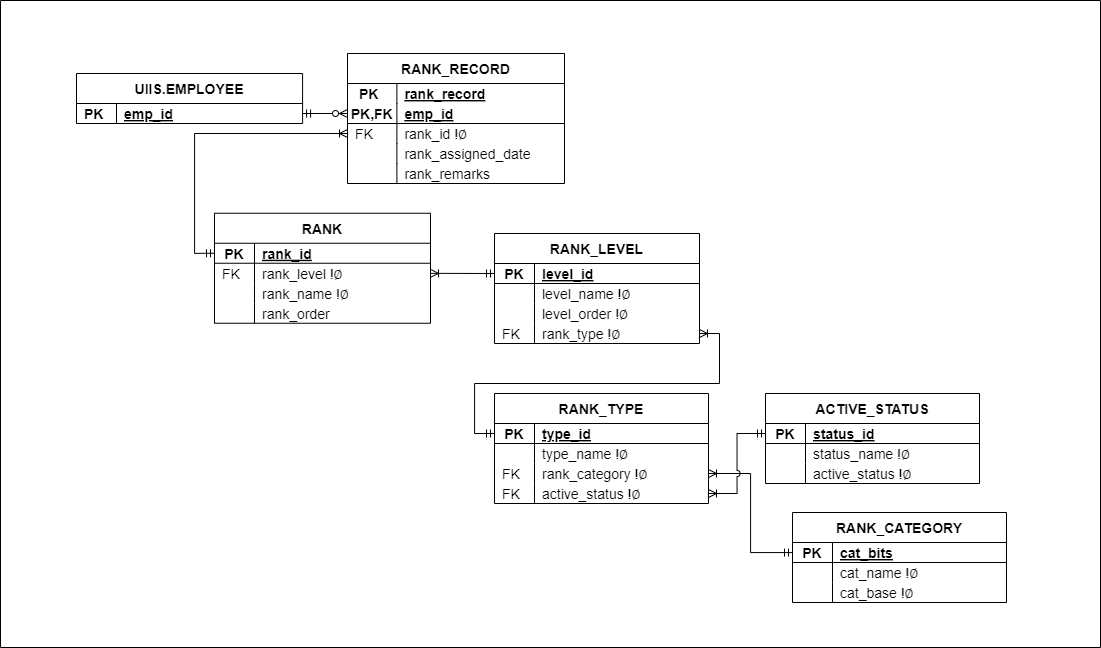
\includegraphics[width=1\linewidth]{figures/images/diagrams/erd/erd-core-rank.png}
        \caption{HRIS Core: Employee Rank ERD Model.}
        \label{fig:erd-core-rank}
    \end{figure}

    The Rank module in this HRIS is designed to manage the hierarchical structure of employee positions within the organization. The central \texttt{hr.rank\_record} entity is directly linked to \texttt{uiis.employee}, associating each employee with their current rank. This entity also connects to the \texttt{hr.rank} entity, which provides details about specific ranks. The \texttt{rank} entity is further linked to \texttt{hr.rank\_level}, allowing for a tiered structure of ranks. \texttt{hr.rank\_level}, then, is associated with \texttt{hr.rank\_type}, which categorizes different types of ranks. The \texttt{hr.rank\_type} entity is connected to both \texttt{hr.rank\_category} and \texttt{hr.active\_status}, enabling the system to classify ranks into broader categories and track their current status. 
            
    This hierarchical structure allows for detailed management of employee rankings, supports career progression tracking, and can facilitate reporting on organizational structure and employee distribution across different rank levels and categories.
    
    \begin{figure}[H]
        \centering
        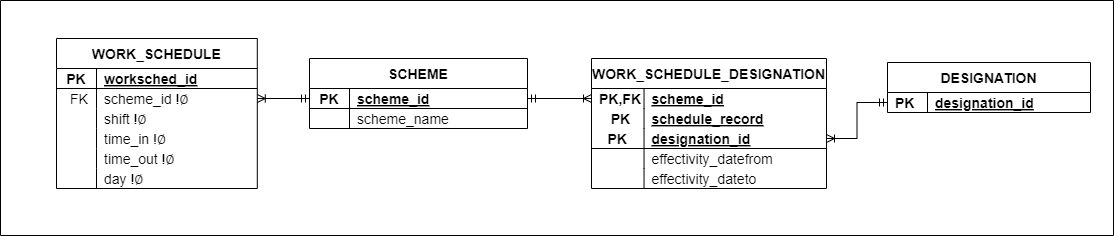
\includegraphics[width=1\linewidth]{figures/images/diagrams/erd/erd-timesys-work-schedule-scheme-and-assignment.png}
        \caption{HRIS TIMESYS: Work Schedule and Assignment ERD Model.}
        \label{fig:erd-timesys-work-schedule-scheme-and-assignment}
    \end{figure}

    The work schedule scheme and assignment module in the HRIS TIMESYS is designed to manage employee work schedules and assignments. The HR manages employee schedules by first defining schemes with assigned work schedules, shift, time-in/out, and day. The HR then assigns these scheme unto the employee under \texttt{hr.work\_schedule\_scheme\_designation}. This work schedule shall be used in reference for other tables within the schema.

    \begin{figure}[H]
        \centering
        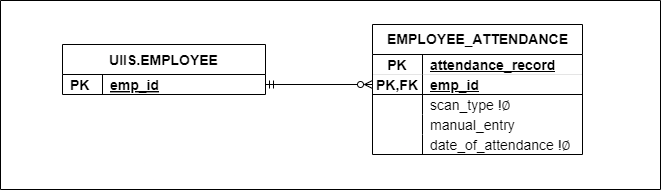
\includegraphics[width=1\linewidth]{figures/images/diagrams/erd/erd-timesys-employee-attendance.png}
        \caption{HRIS TIMESYS: Employee Attendance ERD Model.}
        \label{fig:erd-timesys-employee-attendance}
    \end{figure}

    One of the crucial components of the HRIS TIMESYS module is the employee attendance management system. The structure is designed to capture employee attendance data, including date, time, manual adjustment, and scan types as employees within the University is required to log in their attendance through RFID scanners. The \texttt{hr.employee\_attendance} entity will be the central point for recording not just for recording attendances but will also be used to compute for the employee's tardiness and overtime.

    \begin{figure}[H]
        \centering
        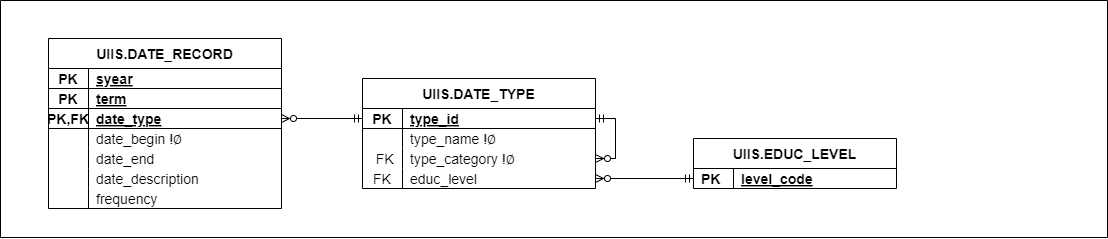
\includegraphics[width=1\linewidth]{figures/images/diagrams/erd/erd-timesys-holiday.png}
        \caption{HRIS TIMESYS: Holiday ERD Model.}
        \label{fig:erd-timesys-holiday}
    \end{figure}

    The holiday module in the HRIS TIMESYS is designed to manage non-working days that should not be counted as absences. The \texttt{hr.date\_record} entity captures detailed information about each holiday, including the date, name, and remarks. The primary purpose for utilizing a customized event management system for holidays is to ensure that employee leave records accurately reflect non-working days. 

    \begin{figure}[H]
        \centering
        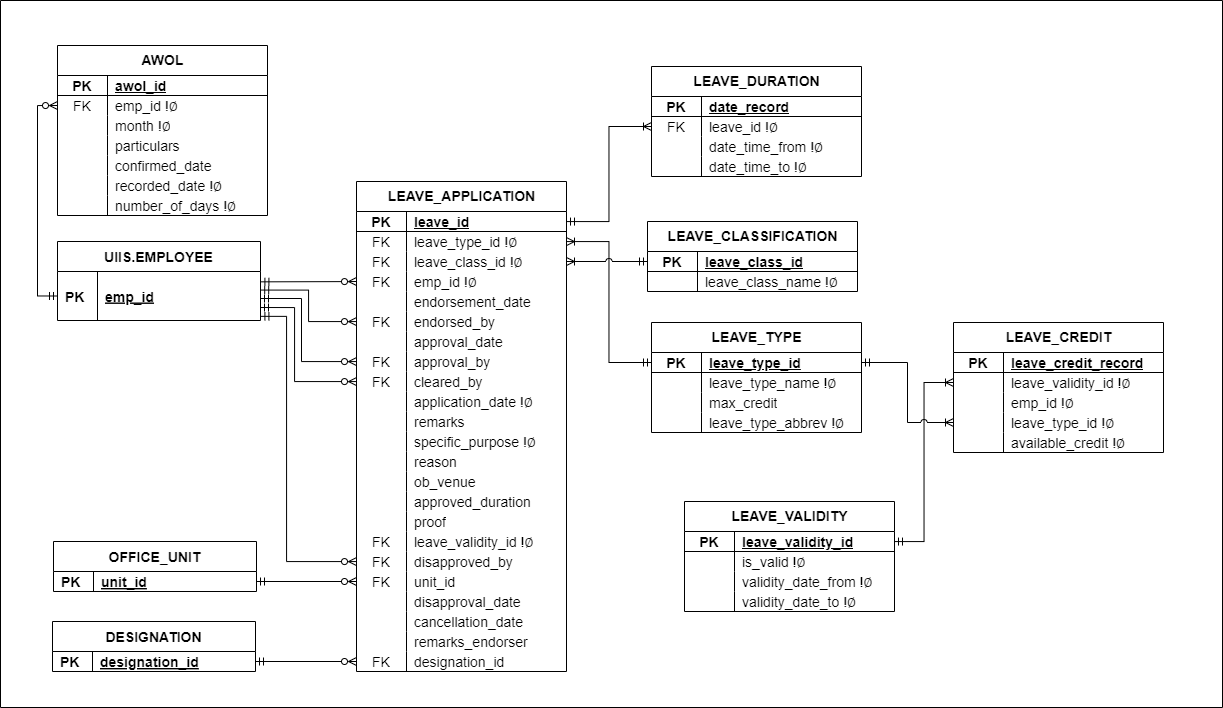
\includegraphics[width=1\linewidth]{figures/images/diagrams/erd/erd-leavesys-employee-leave.png}
        \caption{HRIS LEAVESYS ERD Model.}
        \label{fig:erd-leavesys-employee-leave}
    \end{figure}

    Among the key modules in the HRIS is a module for handling leave applications within the University. This includes handling leave from employees. The \texttt{hr.leave\_application} entity captures detailed information about each leave application, including the date, type, classification, reason, validity, and status. These leaves are then computed and deducted from the employee's leave credits and shall be used upon notifying the employees and for the HR's report.

    The system shall also capture Absent Without Leave (AWOL). The \texttt{hr.awol} entity captures recorded AWOLs, including the date, particulars, confirmed date, and number of days.

    \begin{figure}[H]
        \centering
        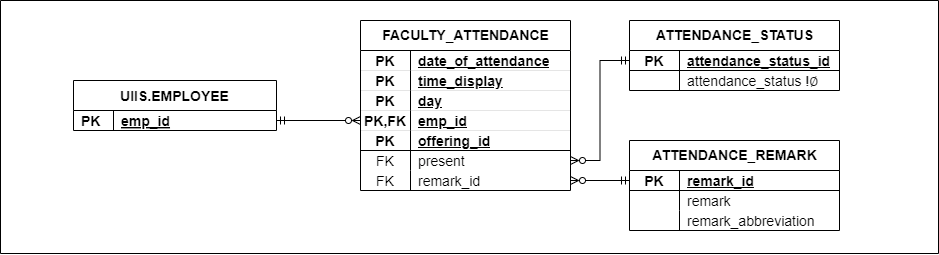
\includegraphics[width=1\linewidth]{figures/images/diagrams/erd/erd-facsys-faculty-attendance.png}
        \caption{HRIS FACSYS ERD Model.}
        \label{fig:erd-facsys-faculty-attendance}
    \end{figure}

    This segment of the ERD model illustrates the HRIS FACSYS module, which focuses on monitoring and recording faculty attendance. It centers around the \texttt{hr.faculty\_attendance} entity, which records detailed attendance information, including date, time, day, and associated course offerings for each employee. The system links to a separate \texttt{uiis.employee} entity, containing broader employee data. It incorporates two supporting entities: \texttt{hr.attendance\_status} for categorizing attendance and \texttt{hr.attendance\_remark} for additional notes. This structure allows for comprehensive tracking of faculty attendance, supporting multiple class offerings per employee and providing flexibility in recording attendance statuses and remarks. The design enables efficient record-keeping and could facilitate various attendance-related analyses and reports.

    \begin{figure}[H]
        \centering
        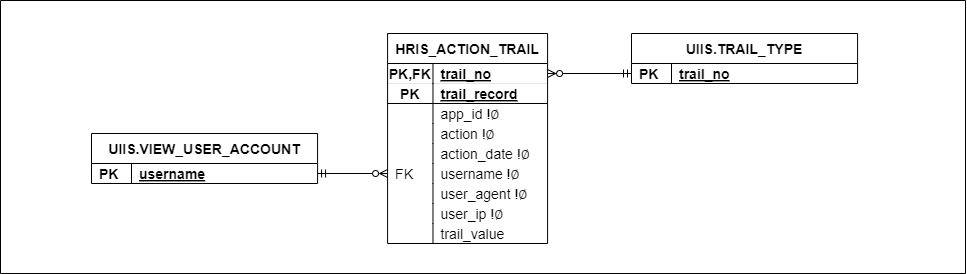
\includegraphics[width=1\linewidth]{figures/images/diagrams/erd/erd-trails.png}
        \caption{HRIS Trails ERD Model.}
        \label{fig:erd-trails}
    \end{figure}

    In order to ensure data integrity and accountability, the new HRIS shall incorporates trails that can tracks all system activities and changes. The trail captures the various entities involved in various modules The \texttt{HRIS\_TRAIL\_ACTION\_TRAIL} entity records the details of each system activity, including the action taken, the entity affected, and the user responsible. This allows for robust monitoring not just for HRMO but also for MIS and DBA to track system activities, changes, and user interactions. 

    This ERD has been reviewed and approved by the MIS DBA with a signed proof of acknowledgement in figure \ref*{fig:proof-ack-erd-consultation} during consultation for this ERD. 
    
    \subsection{Gantt Chart}
    
    Gantt chart allows for a visual representation of the project schedule that outlines the tasks, milestones, and dependencies throughout the development time. In connection with the development of project management strategy through RAD, the HRIS application's use of a Gantt chart will help in planning and tracking the project's progress. It will break down the development process into specific tasks, assign responsibilities, and establish timelines for each phase of the project.
    
    With this, the development team can effectively manage resources, monitor progress, and ensure that the project stays on track to meet the specified deadlines.

    \begin{figure}[H]
        \centering
        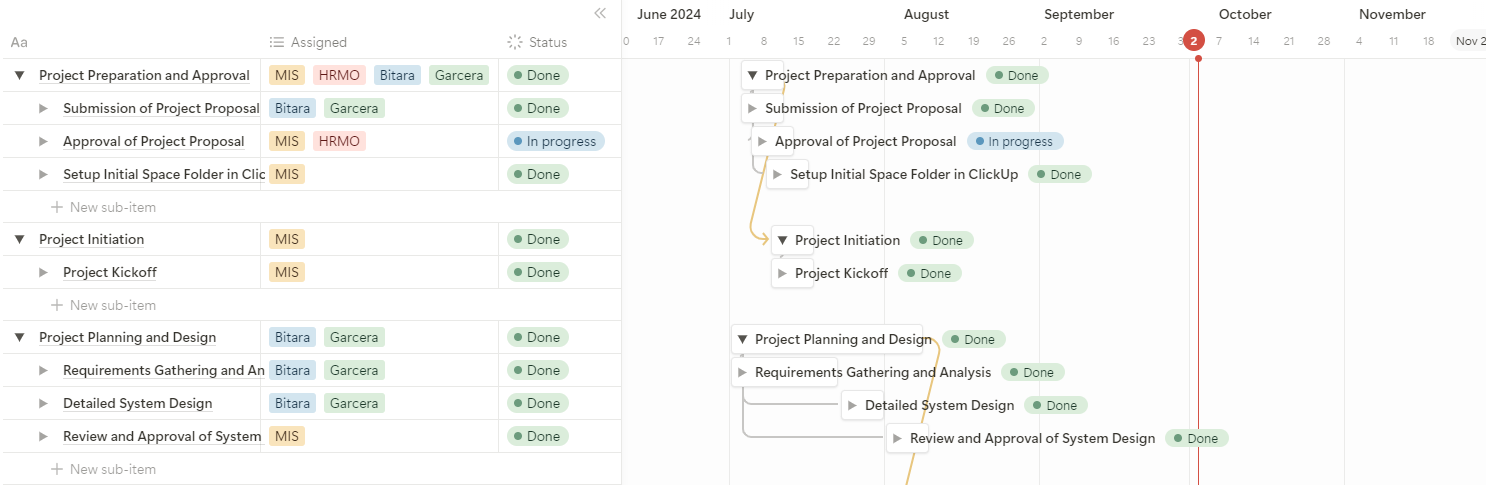
\includegraphics[width=1\linewidth]{figures/images/diagrams/gantt/gantt-chart-1.png}
        \caption{HRIS Gantt Chart Pre-planning Timeline.}
        \label{fig:gantt-chart-1}
    \end{figure}

    The gantt chart in figure \ref{fig:gantt-chart-1} illustrates the pre-planning timeline for the HRIS project. It outlines the key tasks and milestones that need to be completed before the development phase begins. This includes submission and approval of the project proposal, project management setup, to requirements gathering and system design. The timeline provides a clear overview of the project's initial stages and sets the foundation for the subsequent development phases.

    \begin{figure}[H]
        \centering
        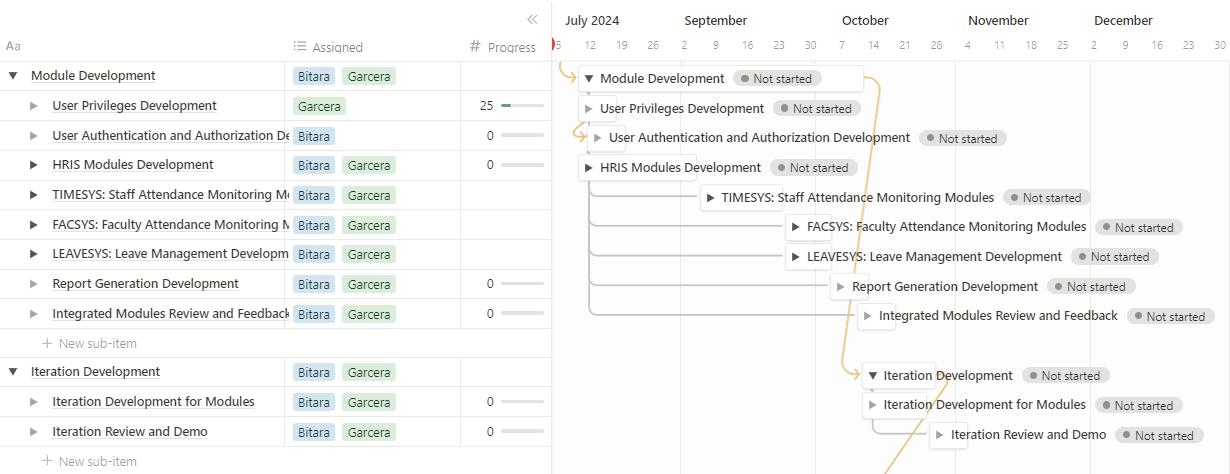
\includegraphics[width=1\linewidth]{figures/images/diagrams/gantt/gantt-chart-2.png}
        \caption{HRIS Gantt Chart Modules Development Timeline.}
        \label{fig:gantt-chart-2}
    \end{figure}

    In the figure \ref{fig:gantt-chart-2}, the gantt chart outlines the timeline for the modules development phase of the project. It breaks down the development process into specific tasks and assigns responsibilities to the development team. The timeline includes tasks from the user authentication to HR core modules, to TIMESYS, LEAVESYS, and FACSYS. During the development phase of the project, the developers shall also make iterations and adjustments based on user feedback and testing results.

    \begin{figure}[H]
        \centering
        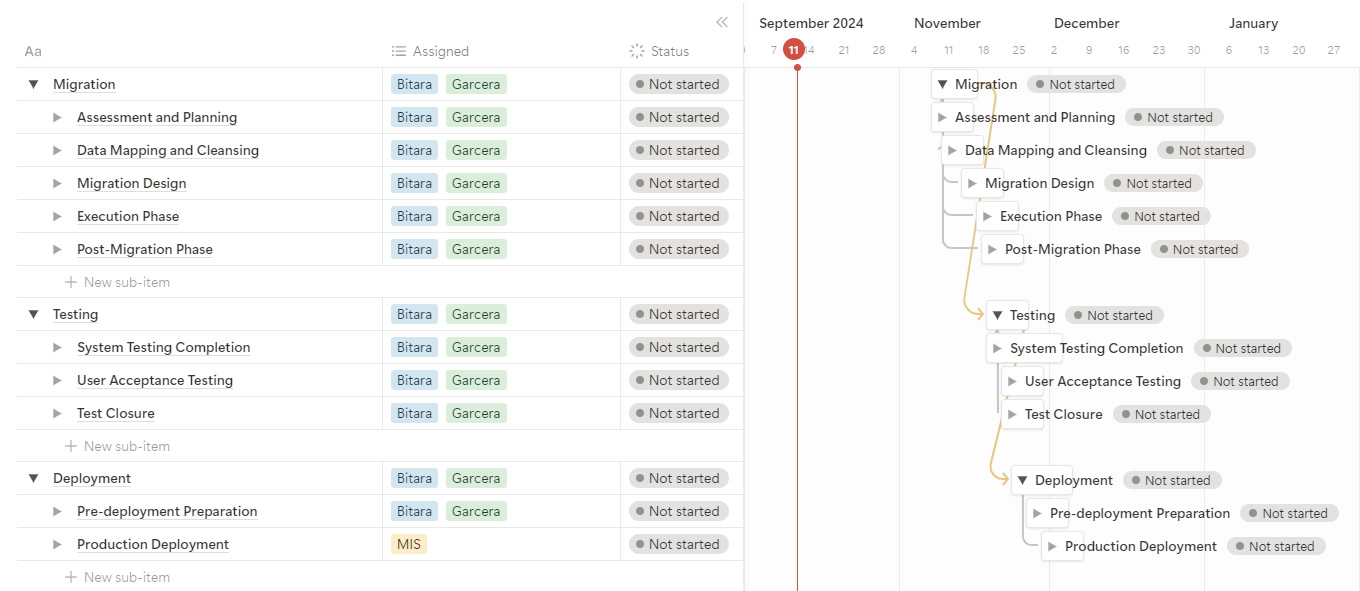
\includegraphics[width=1\linewidth]{figures/images/diagrams/gantt/gantt-chart-3.png}
        \caption{HRIS Gantt Migration to Deployment Timeline.}
        \label{fig:gantt-chart-3}
    \end{figure}

    In the figure \ref{fig:gantt-chart-3}, the gantt chart outlines the timeline for the migration phase of the project. Wherein, it will require other entities such as the HR, ISS, DBA, and MIS to work together to ensure a smooth transition of data from the existing HRIS system to the new HRIS application. The timeline includes migration plan, testing phase, and deployment phase.

    \begin{figure}[H]
        \centering
        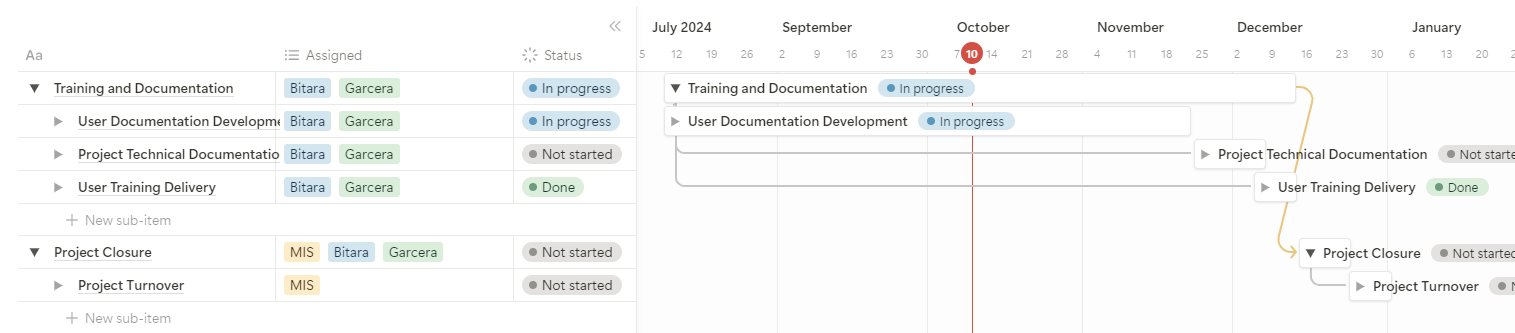
\includegraphics[width=1\linewidth]{figures/images/diagrams/gantt/gantt-chart-4.png}
        \caption{HRIS Gantt Post Development Timeline.}
        \label{fig:gantt-chart-4}
    \end{figure}

    After the deployment phase, the gantt chart in figure \ref{fig:gantt-chart-4} outlines the timeline for the post-development phase of the project. This includes creating trainings and documentations for the HRIS application, providing support, and monitoring the system's performance e.g., user manual, user trainings, and technical documentations. Once accomplished, the project will be handed over to MIS for further management and maintenance.

\section{Data Migration Plan}

    \subsection{Objectives}

    The data migration plan aims to ensure a smooth and efficient transition of data from the existing HRIS system to the new HRIS application. The key objectives of the data migration plan include:

    \begin{enumerate}
        \item Identify and extract relevant data from the existing HRIS system.
        \item Transform and map the data to align with the new HRIS database schema.
        \item Load the data into the new HRIS application while ensuring data integrity and accuracy.
        \item Validate the migrated data to ensure completeness and consistency.
        \item Minimize downtime and disruptions to the HR operation.
        \item Document the data migration process and outcomes for future reference.
    \end{enumerate}

    \subsection{Data Migration Strategy}

    The data migration strategy will involve the following key steps:
    
        \subsubsection{Assessment and Planning}
            This phase involves identifying the key stakeholders, analyzing the current HRIS that being utilized, gathering requirement for the new system. Having a proper assessment and planning are crucial in understanding the scope of the migration, identifying potential risks, and setting clear objectives. This phase ensures that all stakeholders are aligned and that the migration plan addresses all necessary aspects of the project. Also, effective planning will help mitigate risks and lays a solid foundation for the migration process.

        \subsubsection{Data Mapping and Cleansing}
            In this phase, it includes aligning the data fields from the legacy system to the new HRIS and correcting data quality issues. To ensure that all important data is correctly transferred to the new system, having an proper or accurate data mapping is needed. This phase also includes data cleansing as it is essential for maintaining data integrity and ensuring that the new system operates with accurate and reliable data. This step is critical for preventing data-related issues post-migration and ensuring a smooth transition.

        \subsubsection{Migration Design}
            The Migration design involves selecting migration tools  and deciding on the migration approach. Choosing the necessary and right tools and approach can significantly reduce the risk of errors and downtime. With a well-designed migration process ensures that data is transferred efficiently and securely. This step is important for optimizing the migration process and ensuring that it aligns with the project's goals and constraints
        
    \subsection{Execution Phase}
        \subsubsection{Pilot Migration}
            Conducting a pilot migration involves setting up a test environment and performing a trial run with a subset of data. A pilot migration helps identify potential issues and validate the migration process before the full migration. Also, with this step it will be helpful for minimizing risks and ensuring a smooth transition. It allows for adjustments to be made based on the findings from the pilot, thereby improving the overall migration strategy

        \subsubsection{Full Migration}
            In this full migration, it involves extracting, transforming, and loading the full dataset into the new system. Proper execution ensures that all data is accurately transferred and that the new system is ready for use. Validation and reconciliation are essential to confirm data integrity and completeness. This step is the core of the project and requires meticulous planning and execution to ensure success

    \subsection{Post-Migration Phase}
        Post-migration activities include system testing, data validation, user training, and providing support. These activities ensure that the new system operates correctly, that data integrity is maintained, and that users are comfortable with the new system. Ongoing support helps address any issues that arise after the migration. This step is crucial for ensuring the long-term success of the new system and for achieving user satisfaction
    
\section{System Testing Plan}

    The system testing phase aims to comprehensively evaluate the functionality, performance, and reliability of the application. To ensure a thorough assessment, we have established the following key objectives within the system testing plan:
    
    \begin{enumerate}
        \item Verify the functionality of all system features and modules.
        \item Ensure the system meets all specified requirements.
        \item Identify and document any bugs or issues.
        \item Validate the system's performance and response times.
        \item Test the user interface for usability and intuitiveness.
        \item Confirm data integrity and security measures.
        \item Assess the system's compatibility with different browsers and devices.
    \end{enumerate}

    \subsection{Participants}

    Throughout the testing phase, the participants will include the HR managers as well as the Information System Administrator, and the DBA Administrators.

    \subsection{Equipment and Hardware Requirements}

    The requirements for using the application is minimal due to its chosen deployed platform -- web. The application will only require any modern device that can access the internet through modern up-to-date browsers; specifically Google Chrome version 96 and above. 
    
    The testing phase will be conducted within University grounds as it will require the University's internal network for it to be accessed. 

\section{System Deployment Plan}

This section contains some of the high-level tasks and considerations that will be addressed during the deployment phase of the newly developed and migrated ADNU HRIS.

    \subsection{Deployment Planning}
        
        The deployment plan identifies the requirements and responsibilities of both the client and the development team in preparation for deployment. This includes accomplishing HR requirements -- HR core modules, TIMESYS, LEAVESYS, and FACSYS after reaching satisfaction within the testing plan.

    \subsection{Resources}
        \subsubsection{Facilities}

        The facilities required for testing and deployment to the new HRIS will be conducted within the HR office grounds equipped with modern computers as well a reliable and high-speed internet connection.

        \subsubsection{Hardware}

        The hardware required for running the application shall include:

        \begin{enumerate}
            \item Desktop Computers/Laptops
            \begin{enumerate}
                \item \textbf{Processor:} Minimum Intel Core i3 or AMD equivalent
                \item \textbf{RAM:} Minimum of 4GB (recommended 8GB or higher)
                \item \textbf{Storage:} Minimum of 128GB (recommended 256GB or higher)
            \end{enumerate}
            
            \item Backup and Recovery Hardware
            \begin{enumerate}
                \item \textbf{Backup Power supply:} This is to avoid downtime during any power outages to ensure uninterrupted workflow. Ensure that there is a Uninterruptible Power Supply (UPS) systems for critical hardware.
                
                \item \textbf{Electric Generators:} This is to for any extend outages that can occur within operations time. This ensures that the University can still cater and be operational despite the outages.
            \end{enumerate}
            
            \item Peripheral Devices
            \begin{enumerate}
                \item \textbf{DTR Scanner:} The HR module TIMESYS will utilize the DTR Scanner for employee attendance purposes.
                \item \textbf{RFID Scanner:} The RFID scanner will be utilized in support for the DTR within HR.
            \end{enumerate}
            
        \end{enumerate}

        \subsubsection{Support Software}

        As the project will utilize Oracle for the data migration, the supported software shall be to use Oracle 12c with instantclient12 installed and sqldeveloper for the database management solution. 

        Being a web-based application, the project requires to run on modern browsers with version 96 and above for Google Chrome. This ensures better up-to-date features and better security patches for each devices.

        \subsubsection{Support Documentation}

        The documentation required to support the application shall include:

        \begin{itemize}
            \item[] \textbf{User Manuals:} Detailed guides for end-users to navigate and utilize the HRIS effectively.
            \item[] \textbf{Technical Documentation:} In-depth documentation for developers detailing the system architecture, database schema, and configuration settings.
            \item[] \textbf{Training Materials:} Resources for training sessions, including slides, and user manuals.
            \item[] \textbf{FAQs and Troubleshooting Guides:} Common issues and their resolutions to assist users and support staff under user manual.
            \item[] \textbf{System Requirements:} Specifications for hardware, software, and network configurations needed to run the new HRIS.
        \end{itemize}

    \subsection{Deployment Strategies}
    
    The project will be deployed through a series of code review, database review, iteration, and installation of the developed app to the server after a series of testing and acceptance to the application. This process involves multiple personnel including the DB Administrator, Senior Application Developer, and Information System Administrator. 
    
    \subsection{Contingencies}
    
    Contingency plans are ensured to mitigate any potential issues that may arise during and after deployment, the following contingency plans will be put in place:

    \begin{itemize}
        \item[] \textbf{Rollback Plan:} A rollback strategy will be developed and practiced for each implementation to revert to the previous system in case of any critical failures during deployment. This includes utilizing version controls and maintaining a full backup of the old system.

        \item[] \textbf{Performance Monitoring:} Includes continuous monitor of system performance post-deployment through feedback and user reports from the HR for any performance degrade.
    \end{itemize}

    \subsection{Compatibility Strategies}
 
    To ensure smooth deployment and integration of the new ADNU HRIS, the following compatibility strategies will be implemented:
    
    \begin{itemize}
        \item[] \textbf{System Compatibility Testing:} Rigorous testing will be conducted to ensure the new HRIS is compatible with existing hardware, software, and network infrastructure at ADNU.
        
        \item[] \textbf{Browser Compatibility:} The web-based application will be tested across multiple browsers and versions to ensure consistent functionality and appearance.
        
        \item[] \textbf{Integration Testing:} Comprehensive testing will be performed to verify seamless integration with other existing systems and databases at ADNU.
        
        \item[] \textbf{Legacy System Compatibility:} Where necessary, interfaces or middleware will be developed to ensure compatibility with any legacy systems that need to interact with the new HRIS.
        
        \item[] \textbf{Scalability Testing:} The system will be tested to ensure it can handle increased load and user numbers as the university grows. This includes data optimization during any reports or querying. 
    \end{itemize}
    
\section{System Snapshots}

This section contains some of the few initial screen mock-ups for redesigning among the major services of the previous HR system. This includes samples of high-fidelity wireframe made in Figma. This allows for better visualization to the expected output for the new ADNU HRIS.

    \begin{figure}[H]
        \centering
        \frame{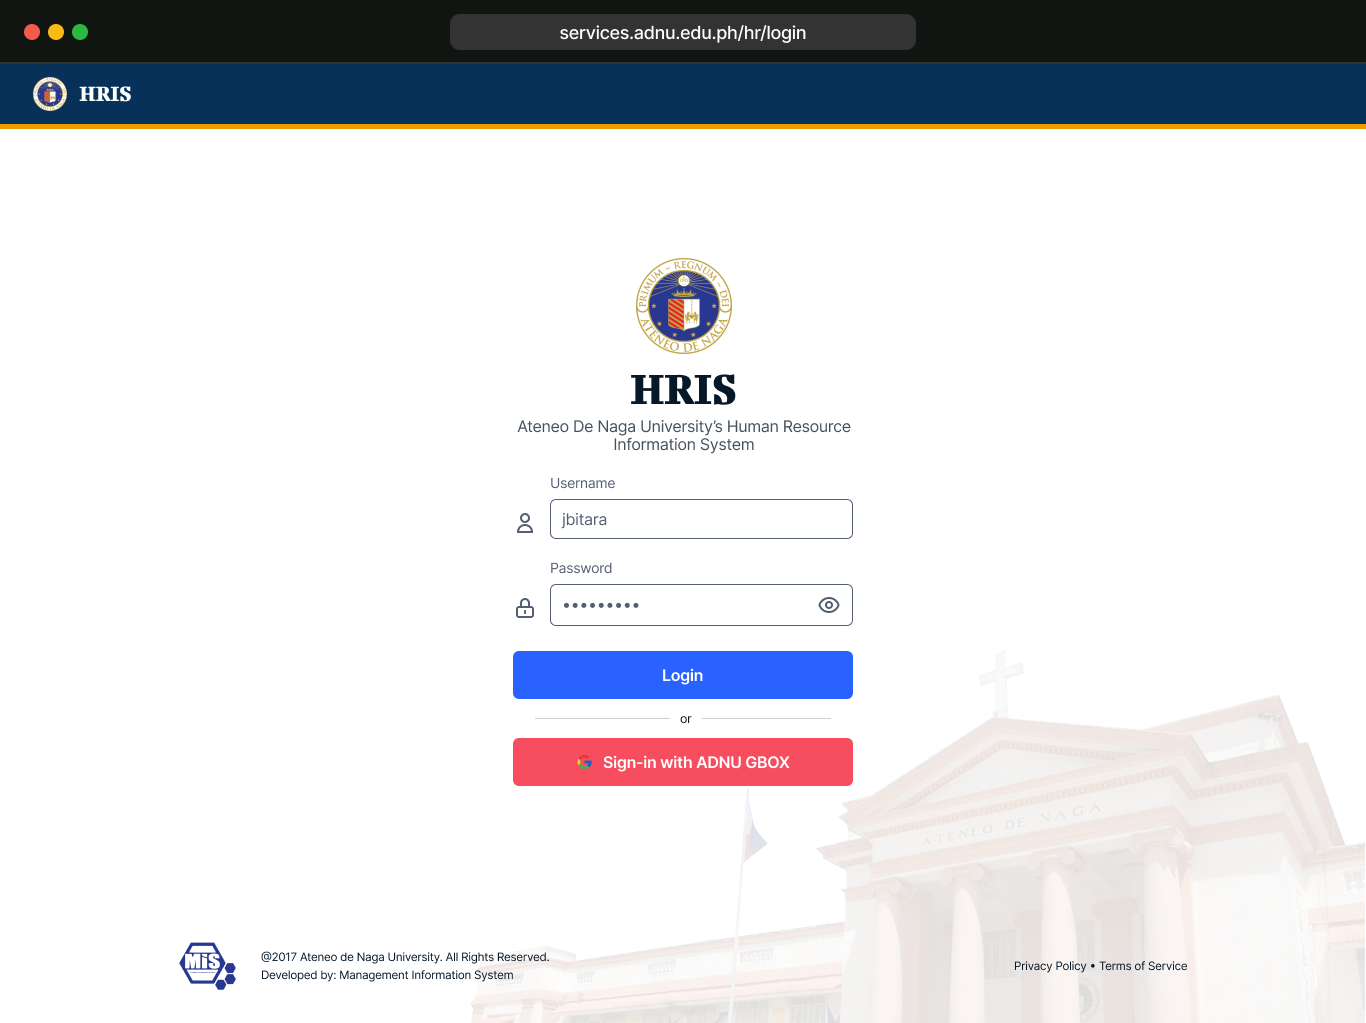
\includegraphics[width=1\linewidth]{figures/app/login.png}}
        \caption{Redesigned Login Page.}
        \label{fig:app-login}
    \end{figure}

    The new HRIS shall include an authentication module to handle HR managers i.e., Director, Administrative Assistant, Capability Building Officer, Compensation \& Benefits Officer, Information Support Systems Officer, Consultant, Recruitment Staff, Training \& Development Specialist, Benefits and Wellness Specialist, Attendance Monitoring Staff, College
    
    Within this page, users can input their University account credentials or login through the use of their GBOX account.

    \begin{figure}[H]
        \centering
        \frame{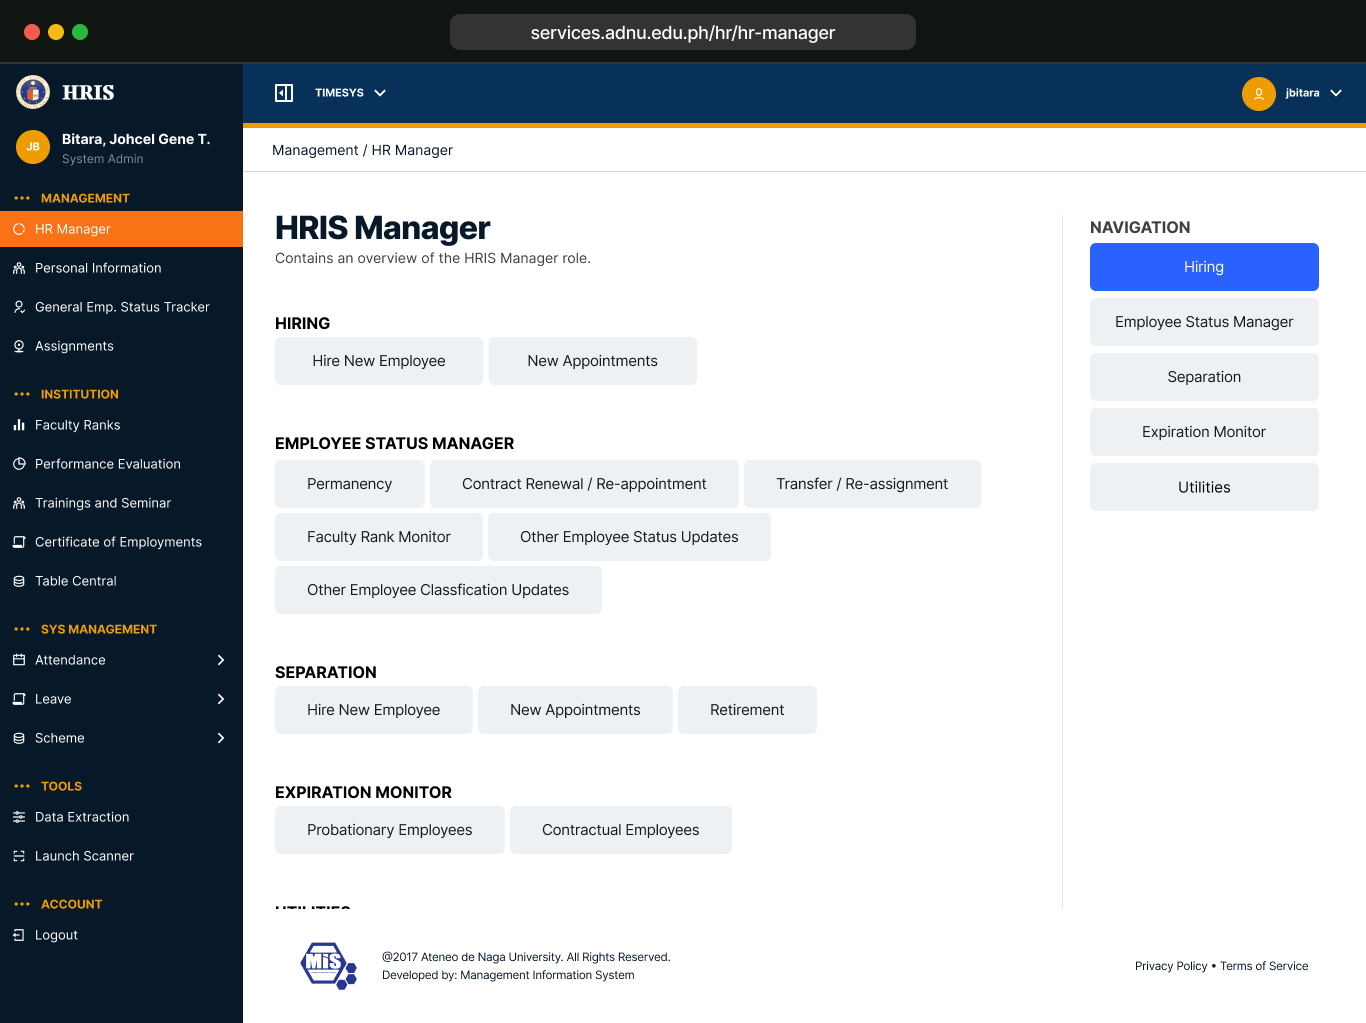
\includegraphics[width=1\linewidth]{figures/app/dashboard.png}}
        \caption{Redesigned Dashboard Page.}
        \label{fig:app-manager}
    \end{figure}

    Within this page, is the default home page for all HR managers. This page displays the summary of the HRIS system and the current status of the HRIS system. This includes a visualized Key Performance Indicators (KPIs) of the system's data and the current status of the system along with clickable links for different modules.

    \begin{figure}[H]
        \centering
        \frame{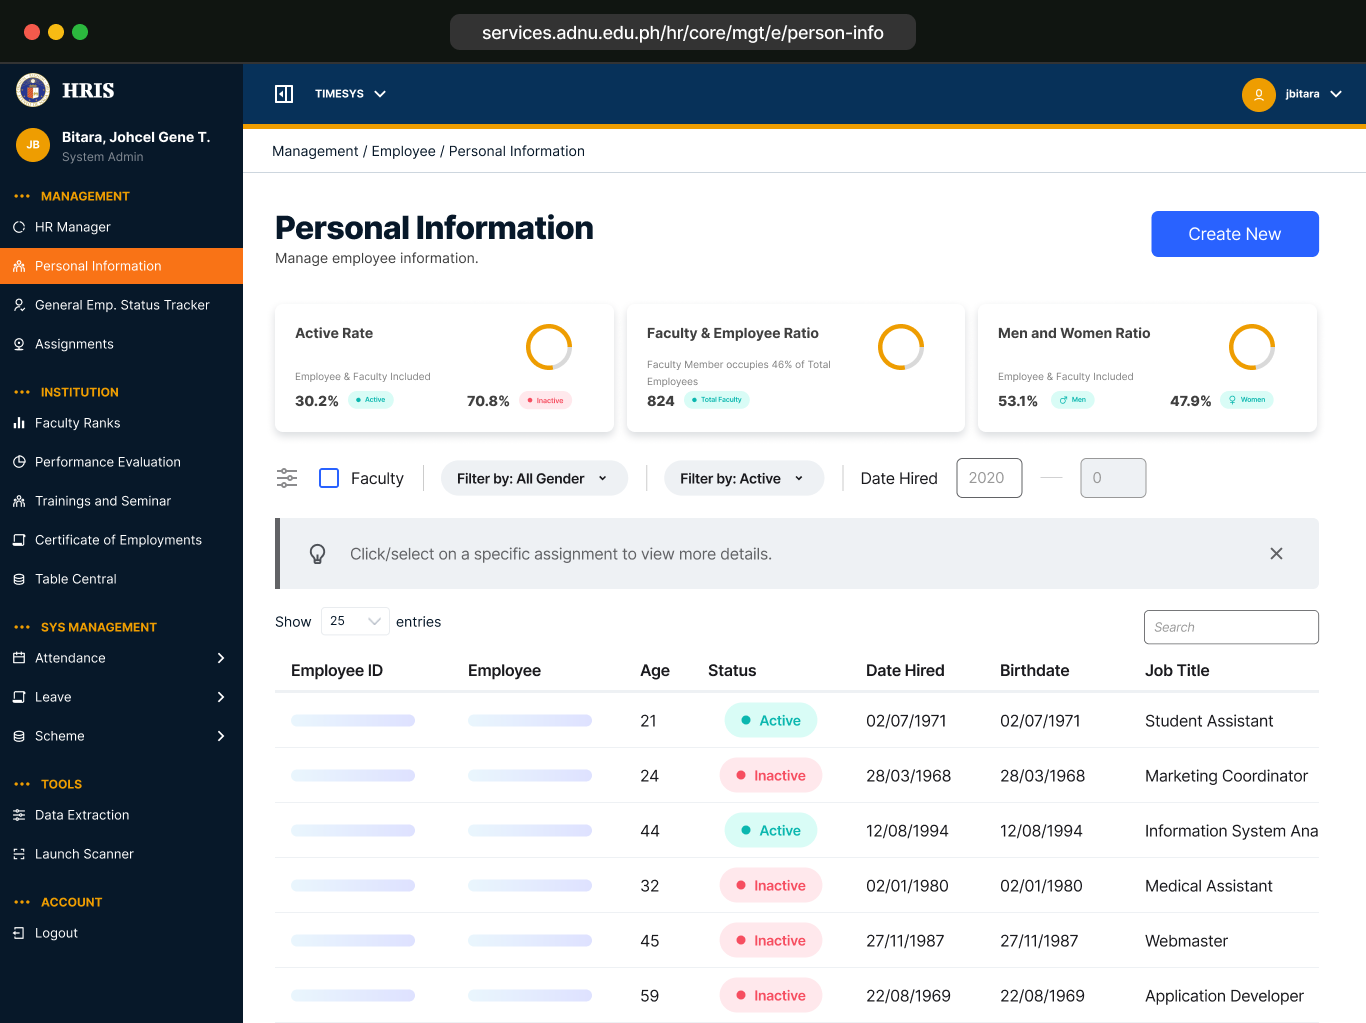
\includegraphics[width=1\linewidth]{figures/app/pi.png}}
        \caption{Redesigned Personal Information for All Employees.}
        \label{fig:app-pi}
    \end{figure}

    Within this page displays all the basic personal information for all employees in table view. This includes their personal information. Admins can select or filter among the employees to view more of their personal information.

    \begin{figure}[H]
        \centering
        \frame{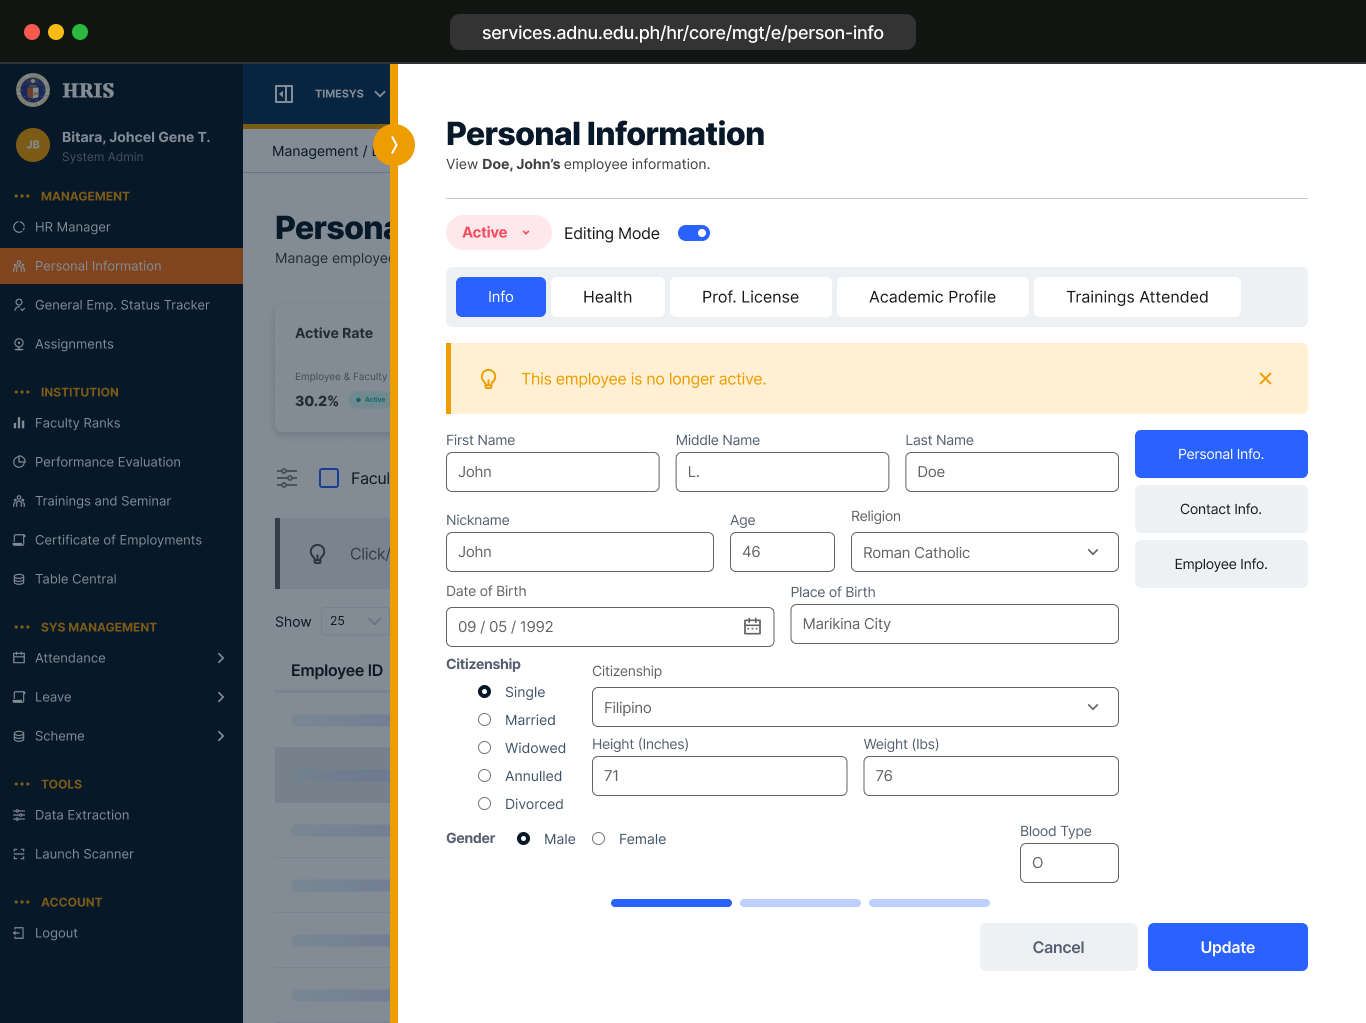
\includegraphics[width=1\linewidth]{figures/app/pi-info.png}}
        \caption{Viewing of Personal Information on Selected Employee.}
        \label{fig:app-pi-info}
    \end{figure}

    Upon selecting an employee, the page displays the interface for viewing/managing of the selected personal information in the record. Admins with access privileges can manage personal information for each employee  in the system.

    \begin{figure}[H]
        \centering
        \frame{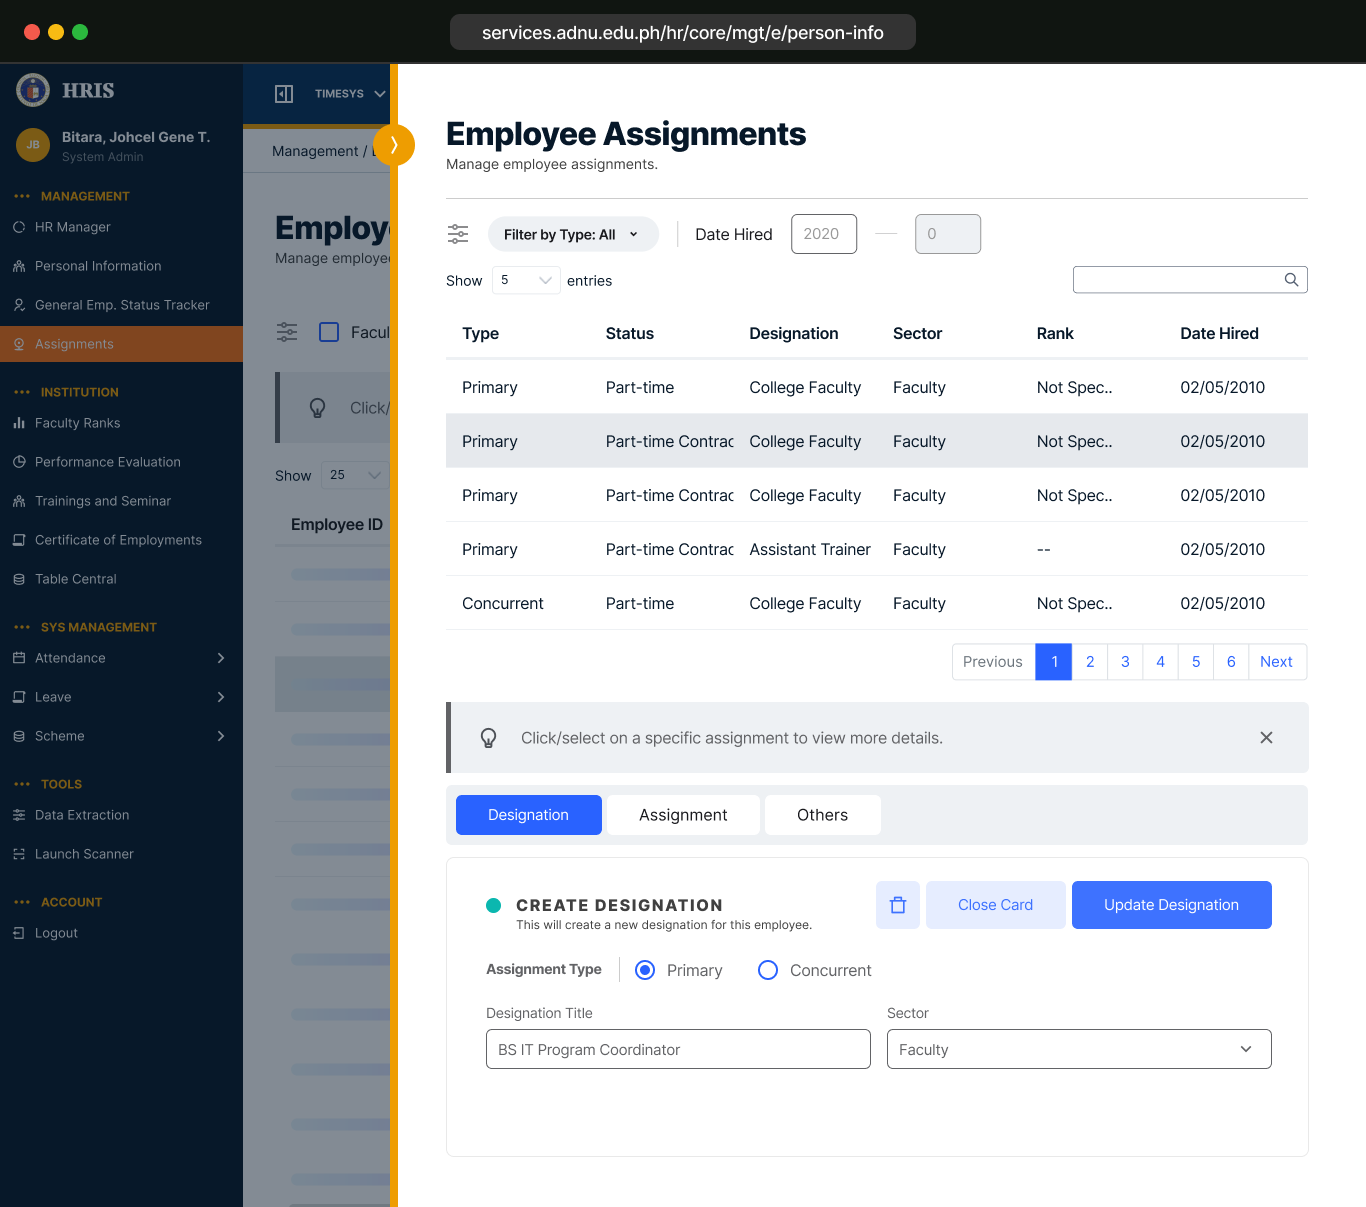
\includegraphics[width=1\linewidth]{figures/app/assignment.png}}
        \caption{Redesigned Employee Assignment Page.}
        \label{fig:app-assignment}
    \end{figure}

    Part of the crucial components of the system is managing employee designations and assignments. This page displays the interface for managing employee assignments and designations. Admins can assign employees to specific roles, office unit designation, create remarks, and employment status.

    \begin{figure}[H]
        \centering
        \frame{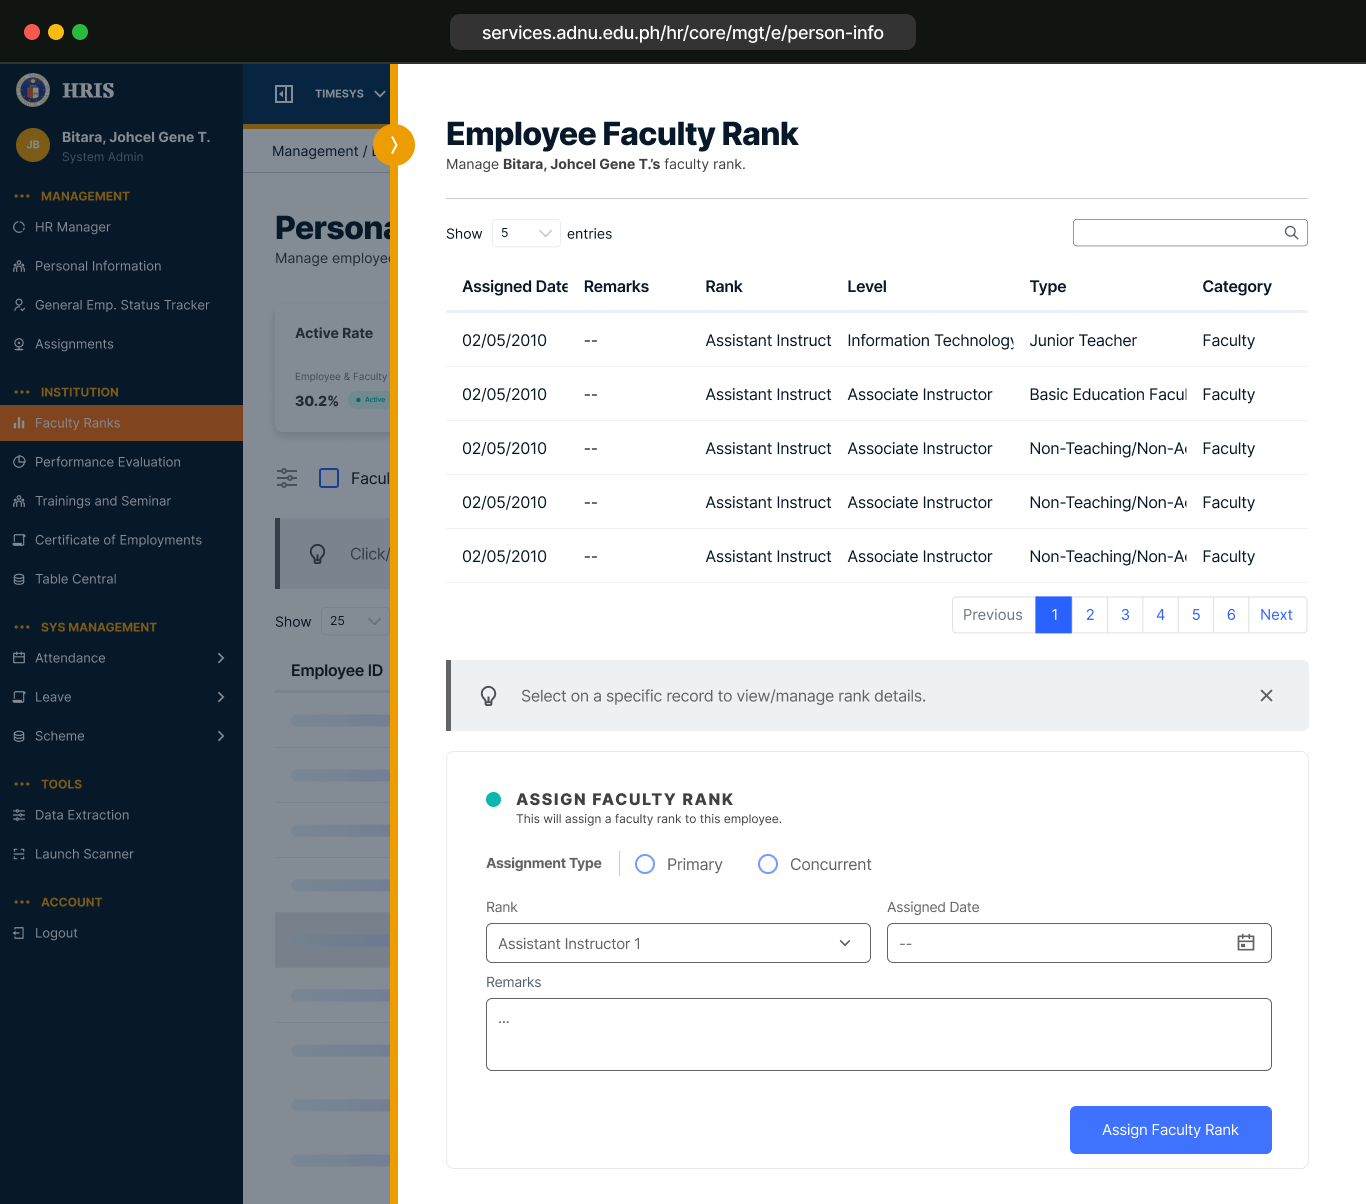
\includegraphics[width=1\linewidth]{figures/app/ranks.png}}
        \caption{Redesigned Faculty Rank Page.}
        \label{fig:app-fac-rank}
    \end{figure}

    This page displays the interface for managing faculty ranks. Similarly with managing employee information and assignments, the admin selects among the table and a sidebar will display the information for the selected faculty member.
    
    Admins can assign faculty members to specific ranks, rank levels, and rank types. This page also includes functionalities for tracking rank changes and historical data.

    \begin{figure}[H]
        \centering
        \frame{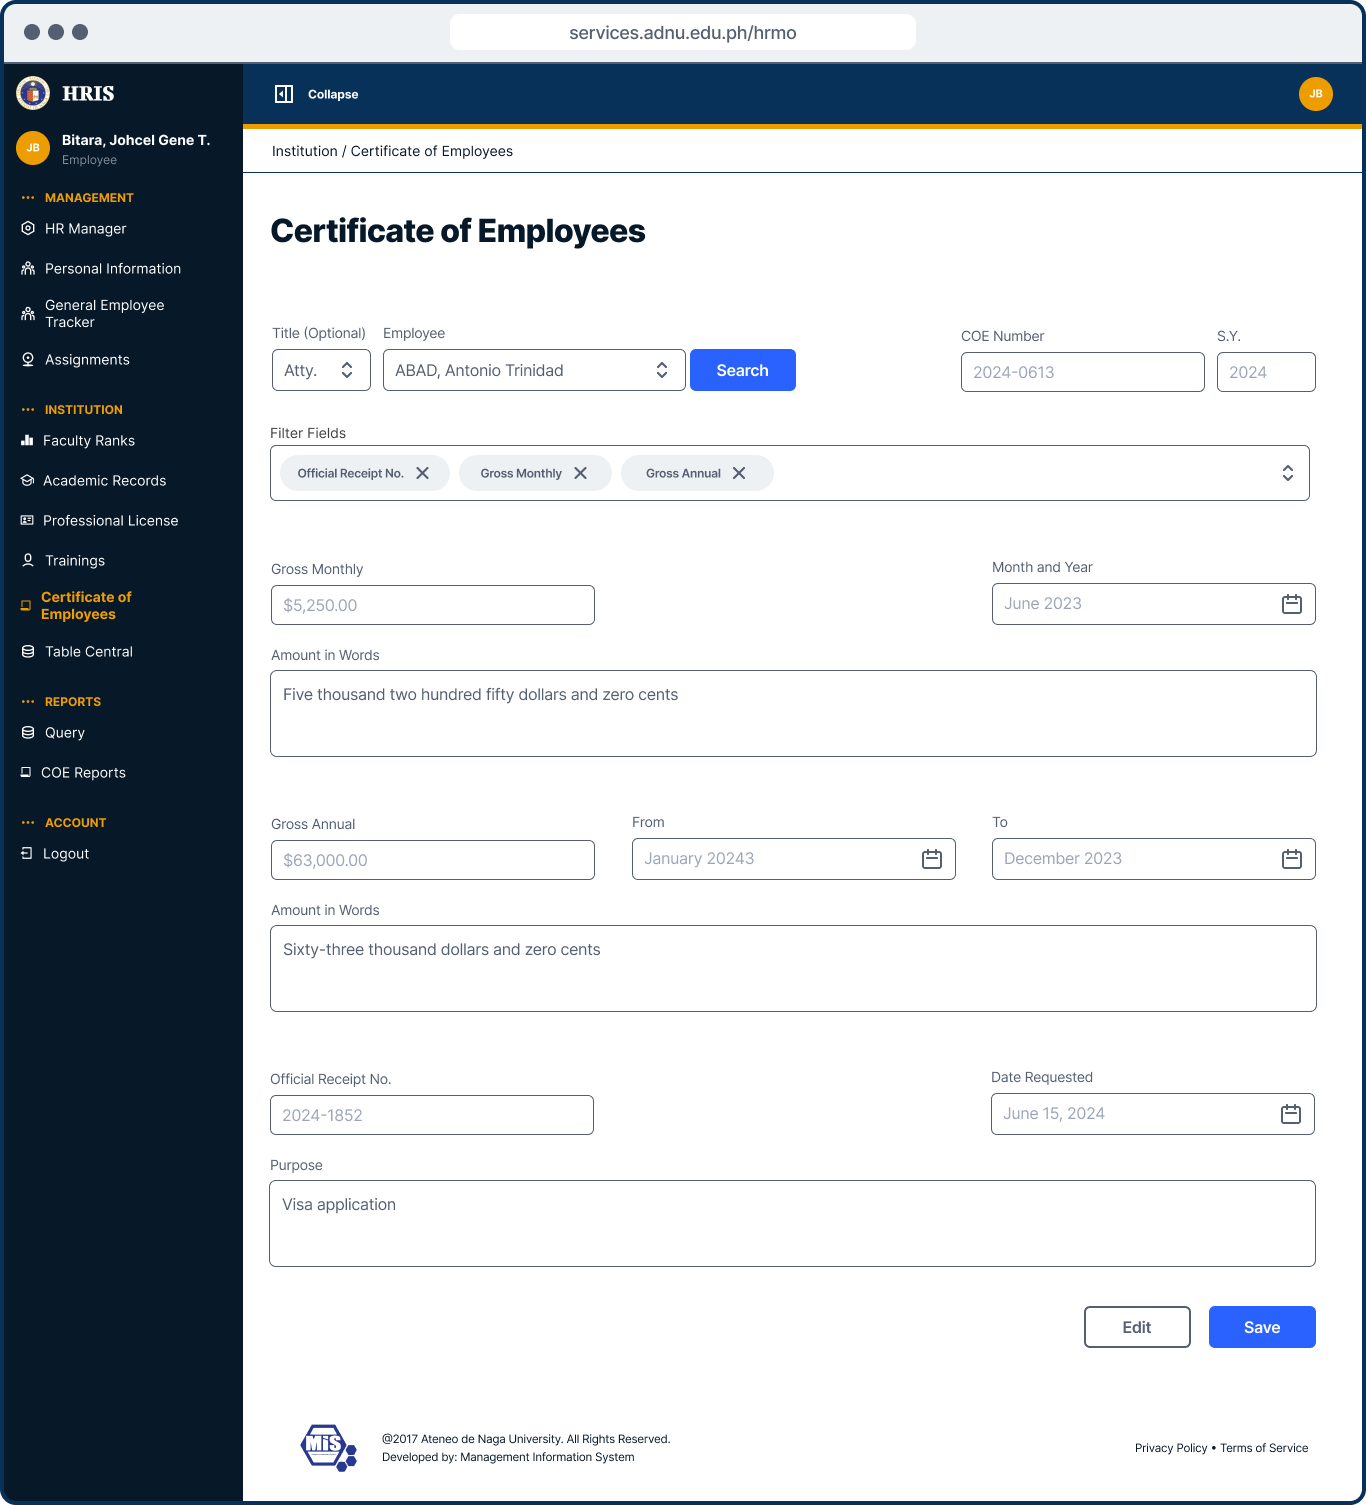
\includegraphics[width=1\linewidth]{figures/app/coe.png}}
        \caption{Redesigned Certificate of Employment Page.}
        \label{fig:app-coe}
    \end{figure}

    This page displays the interface for managing and generating newly issued or history of Certificates of Employment (COE). Within this page, admins can select or filter among the entries from the table and view the details of the selected COE. 

    \begin{figure}[H]
        \centering
        \frame{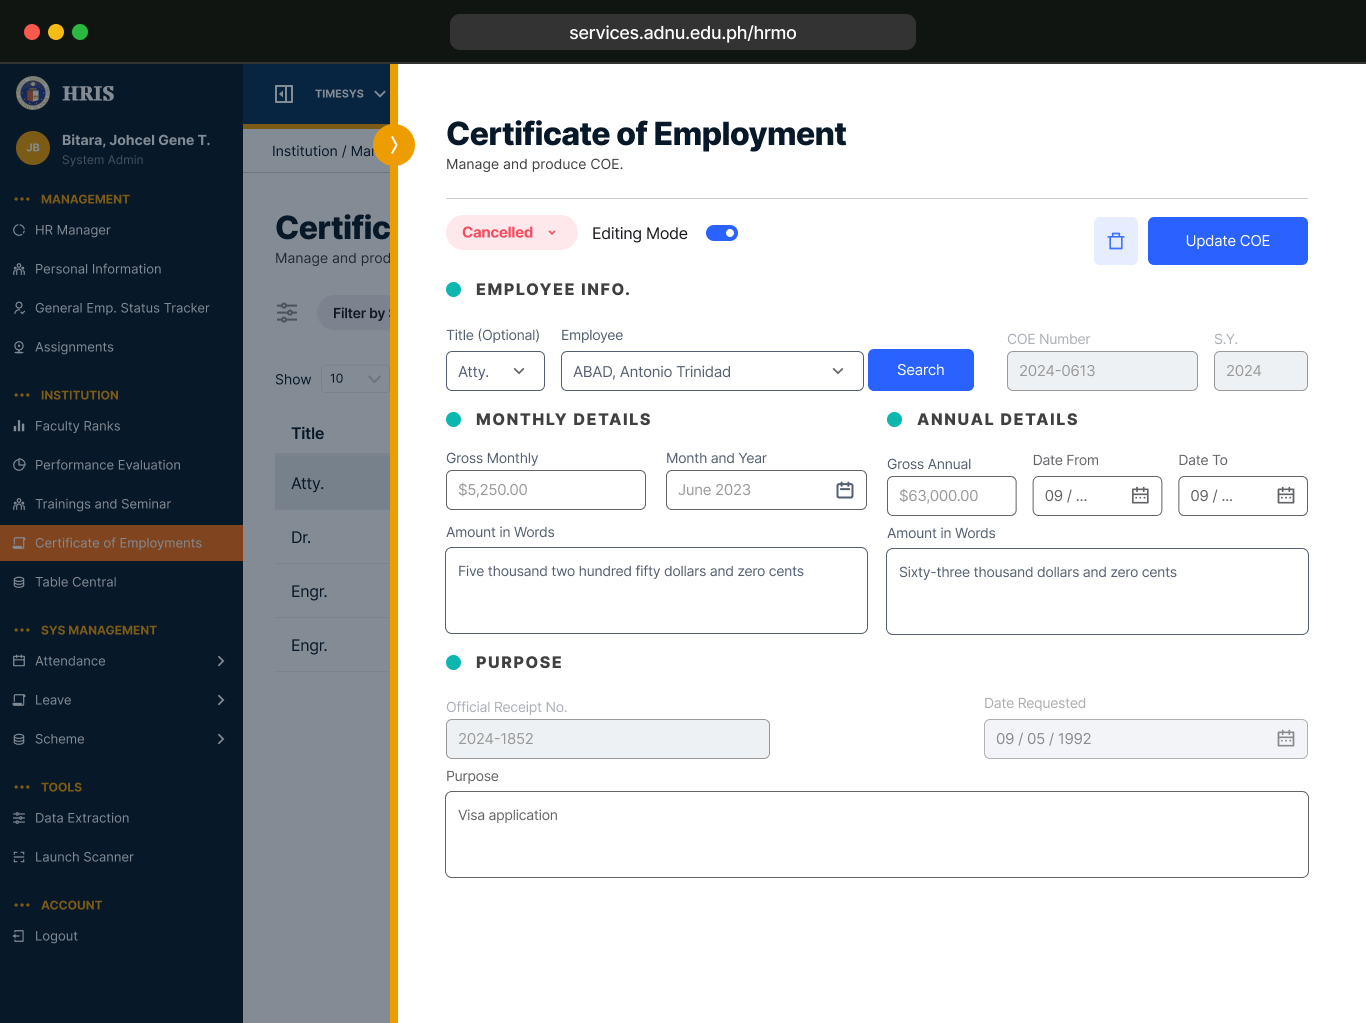
\includegraphics[width=1\linewidth]{figures/app/coe-info.png}}
        \caption{New HRIS Certificate of Employment Processing Page.}
        \label{fig:app-coe-info}
    \end{figure}

    Upon selecting a COE, the page displays the interface for viewing/managing of the selected COE in the record. Admins with access privileges can manage COE information for each employee in the system.

    \begin{figure}[H]
        \centering
        \frame{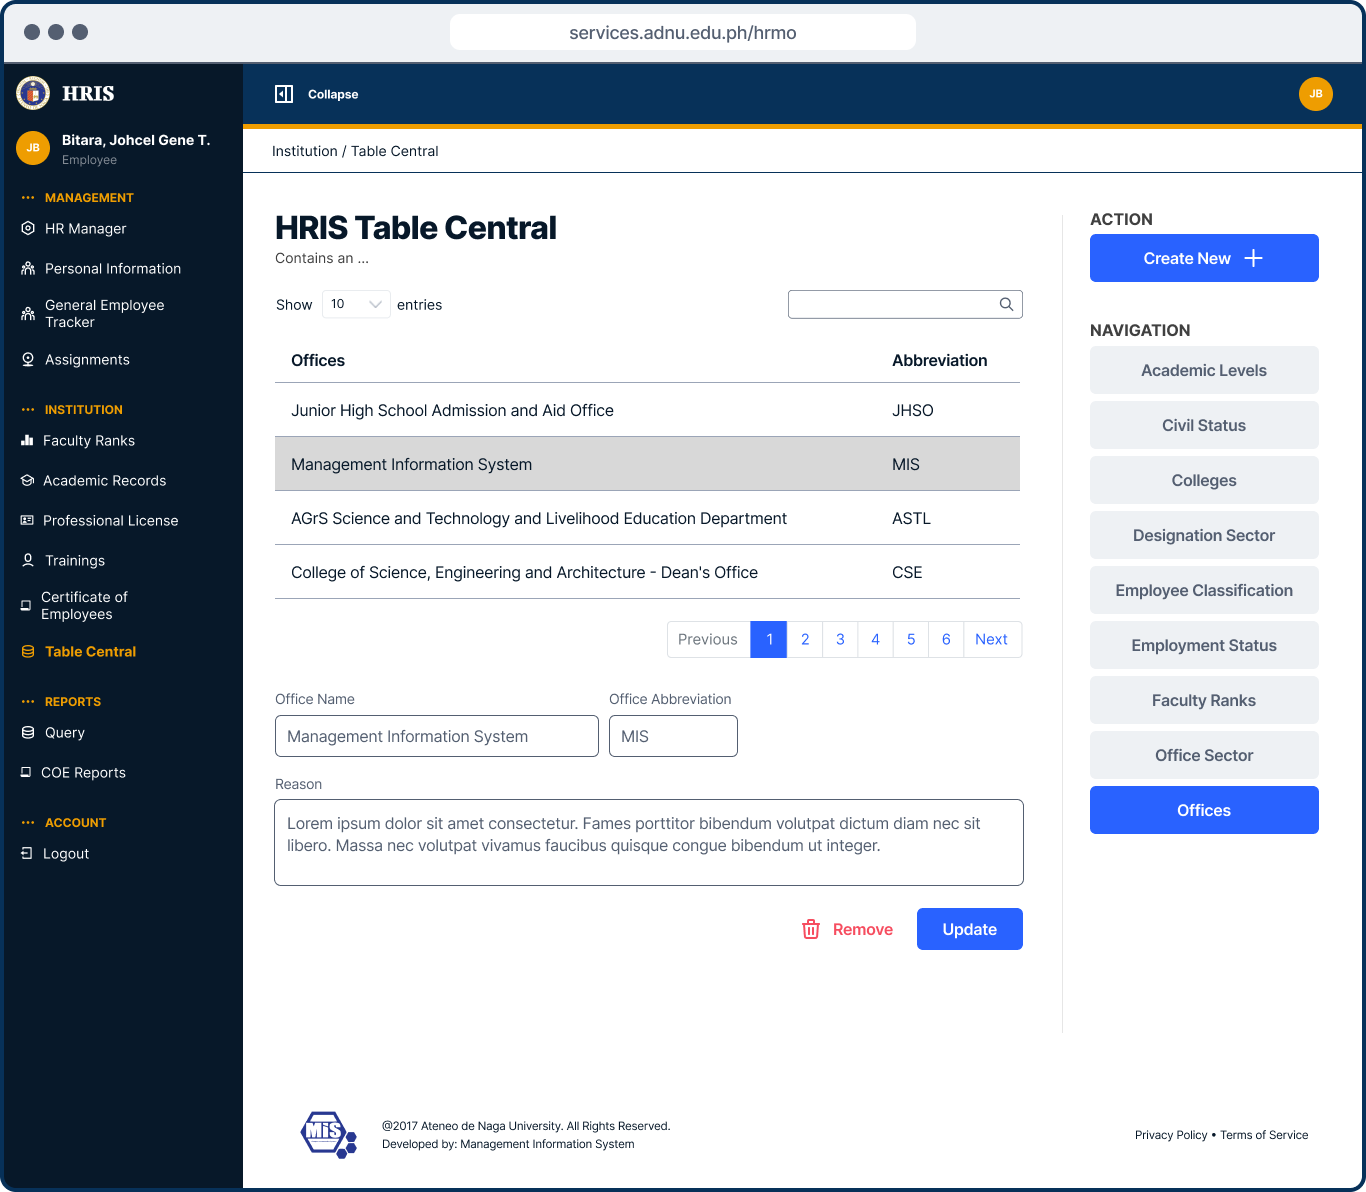
\includegraphics[width=1\linewidth]{figures/app/table-central.png}}
        \caption{Redesigned Table Central Page.}
        \label{fig:app-table-central}
    \end{figure}

    Within this page displays the HRIS Table Central module wherein, managers can manage certain sectors and department information and make updates within the schema's base tables. This includes the office type, office unit, office sector, academic levels, civil statuses, colleges, designation sectors, employee classification, employment status, and faculty ranks. which are used in reference to the HR's data as well on other University's systems.

    \begin{figure}[H]
        \centering
        \frame{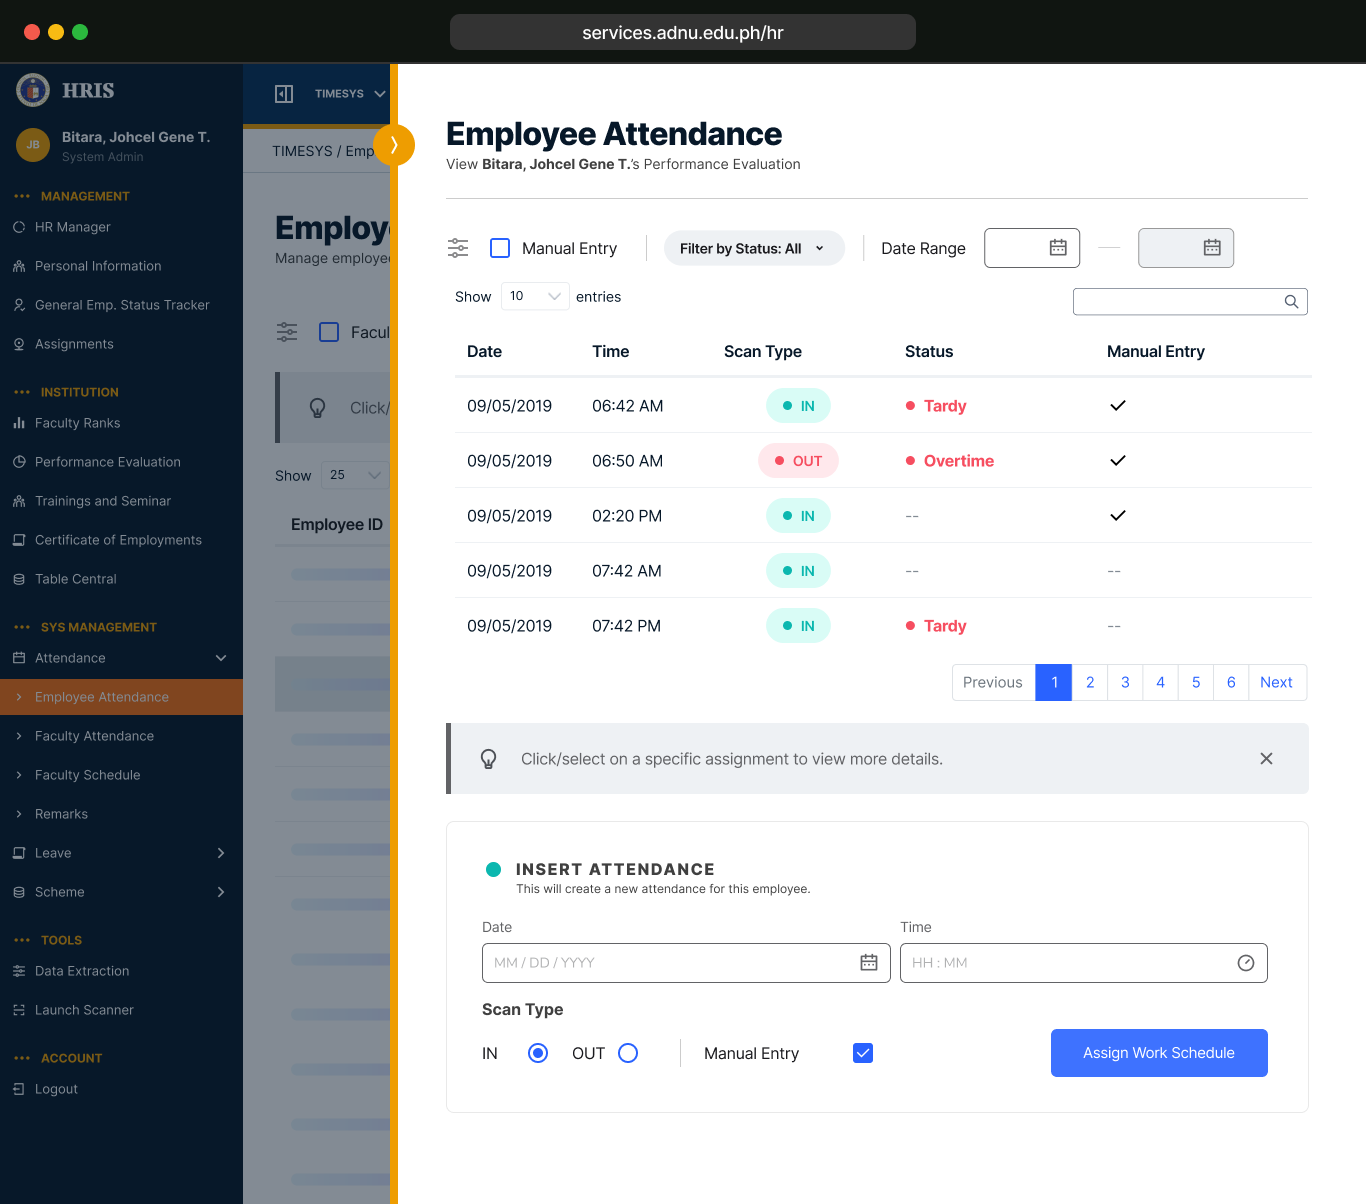
\includegraphics[width=1\linewidth]{figures/app/attendance-emp.png}}
        \caption{Redesigned Employee Attendance Management Page.}
        \label{fig:app-attendance-emp}
    \end{figure}

    Within this page displays the interface for managing employee attendance. This is in connection with the TIMESYS module and the DTR scanner. Records of employee attendance are displayed in table view, and admins can manage attendance records, including time-in/out, date, scan type and their computed status -- Tardy, Overtime, Absent, or Present.

    \begin{figure}[H]
        \centering
        \frame{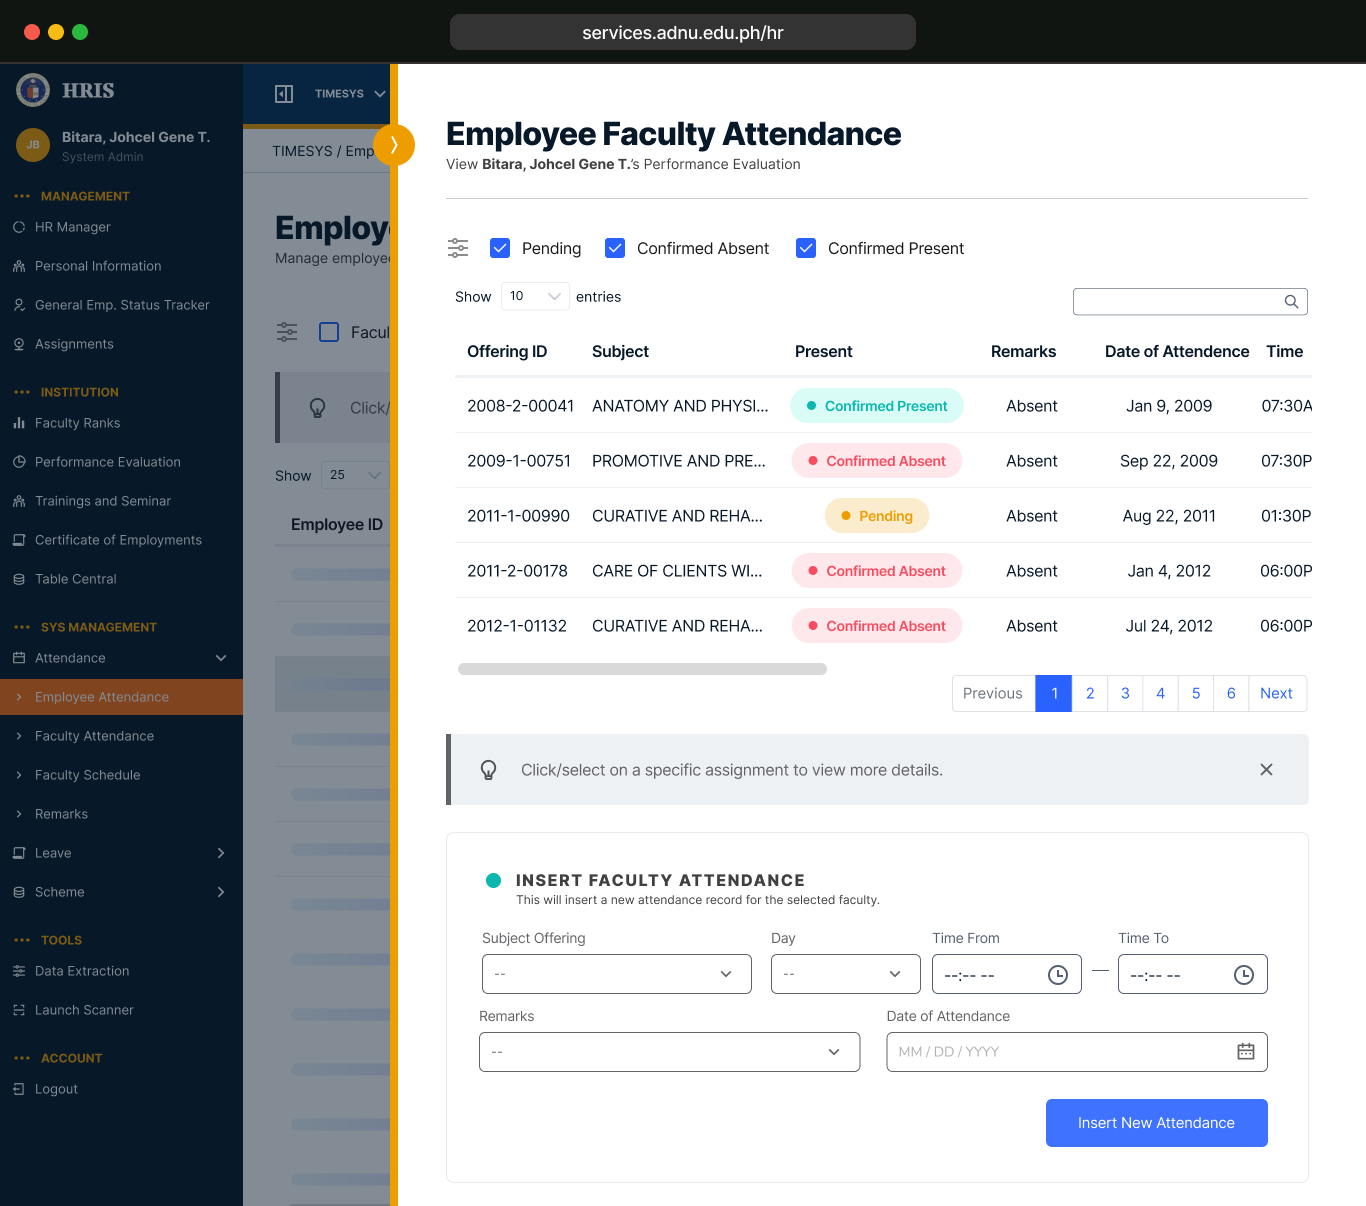
\includegraphics[width=1\linewidth]{figures/app/attendance-fac.png}}
        \caption{Redesigned Faculty Attendance Management Page.}
        \label{fig:app-attendance-fac}
    \end{figure}

    With this page displays the interface for managing faculty attendance. This is in connection with the FACSYS module. Records of faculty attendance are displayed in table view, and admins can manage attendance records, including the subject attended, day, remarks, and date of attendance.

    \begin{figure}[H]
        \centering
        \frame{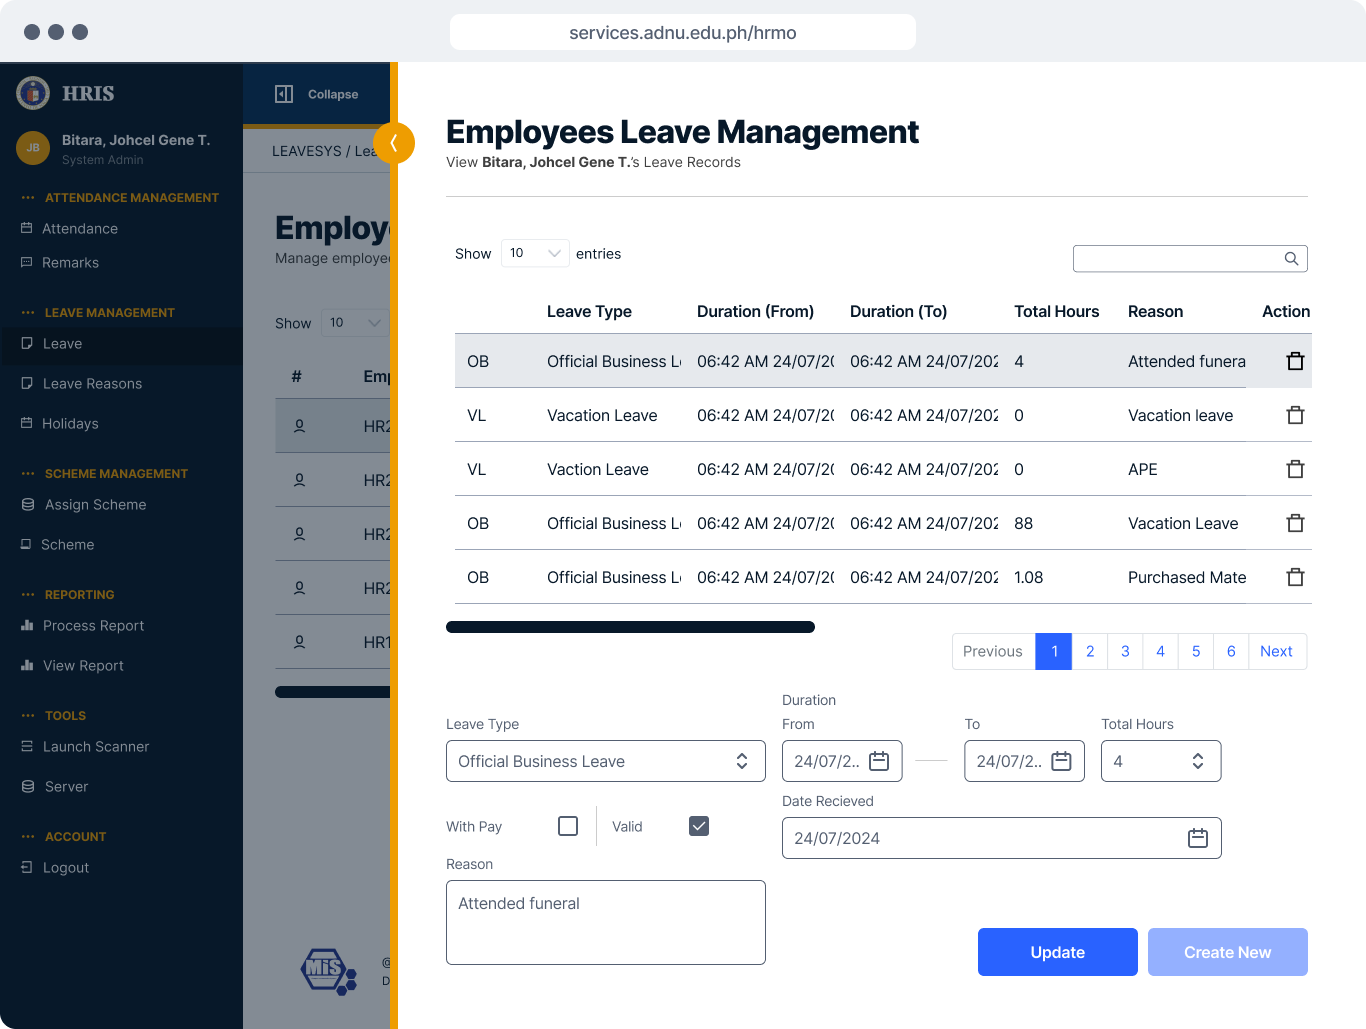
\includegraphics[width=1\linewidth]{figures/app/leave-mgt.png}}
        \caption{Redesigned Leave Management Page.}
        \label{fig:leave-mgt}
    \end{figure}

    Within this page, admins can manage filed employee leave applications and AWOLs. Admins can entry leave applications, view leave applications, and manage leave applications. This page also includes functionalities for tracking leave balances and leave credits of the selected employee.

    \begin{figure}[H]
        \centering
        \frame{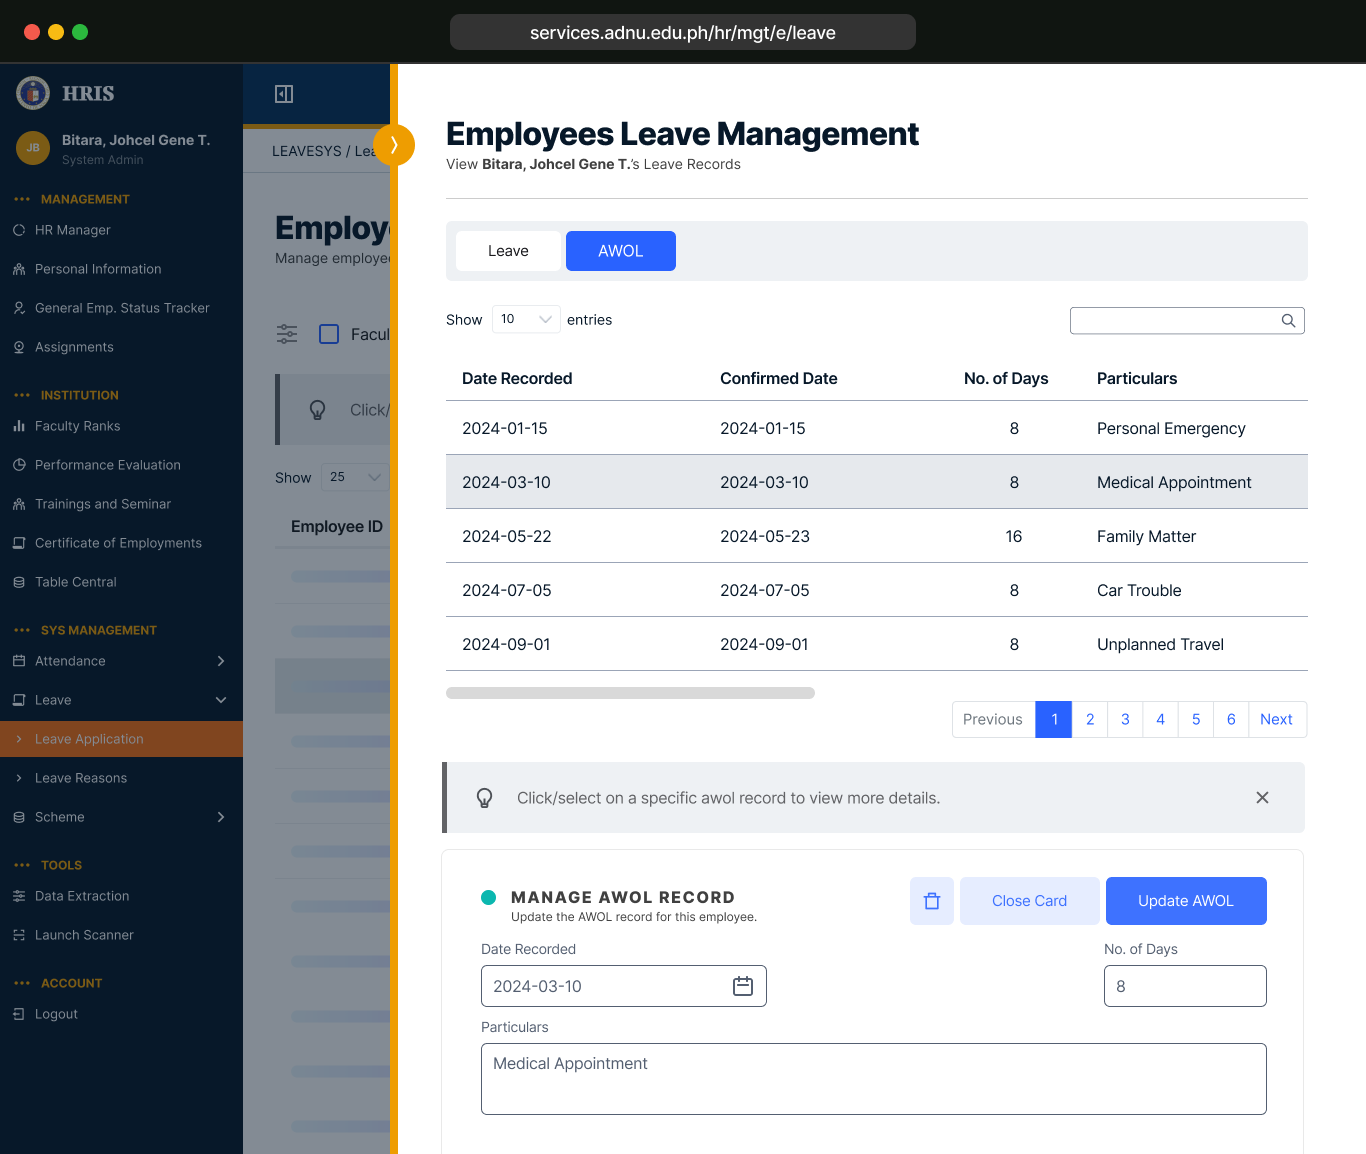
\includegraphics[width=1\linewidth]{figures/app/leave-awol.png}}
        \caption{New HRIS Employee AWOL Page.}
        \label{fig:leave-awol}
    \end{figure}

    Upon switching to the AWOL tab, the page displays the interface for managing and tracking Absent Without Leave (AWOL) records. In this section, admins can view, manage, and track AWOL records, including the date, particulars, confirmed date, and number of days.

    \begin{figure}[H]
        \centering
        \frame{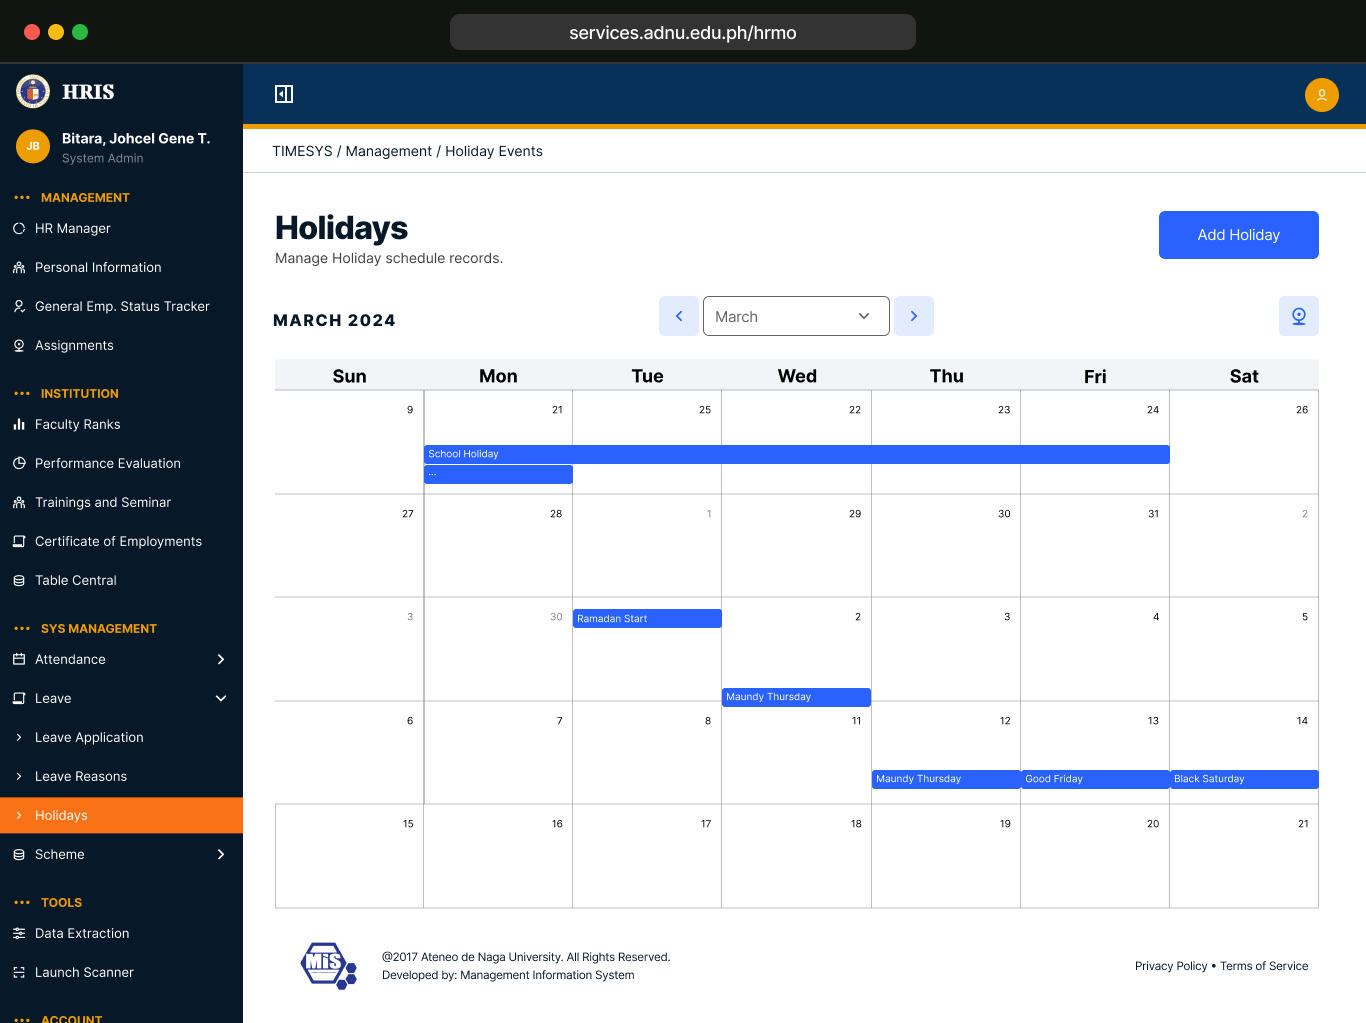
\includegraphics[width=1\linewidth]{figures/app/holiday.png}}
        \caption{Redesigned Holiday Management Page.}
        \label{fig:holiday}
    \end{figure}

    In this page, displays the management for holiday events. The interface provides a comprehensive view of the University's holiday schedules and non-working days. It includes functionalities for managing and updating holiday information with added optimization for their workflow by adding settings for recurrent dates.

    This record is crucial for the LEAVESYS and TIMESYS module as it is used to exclude non-working days from the leave computation and attendance monitoring.

    \begin{figure}[H]
        \centering
        \frame{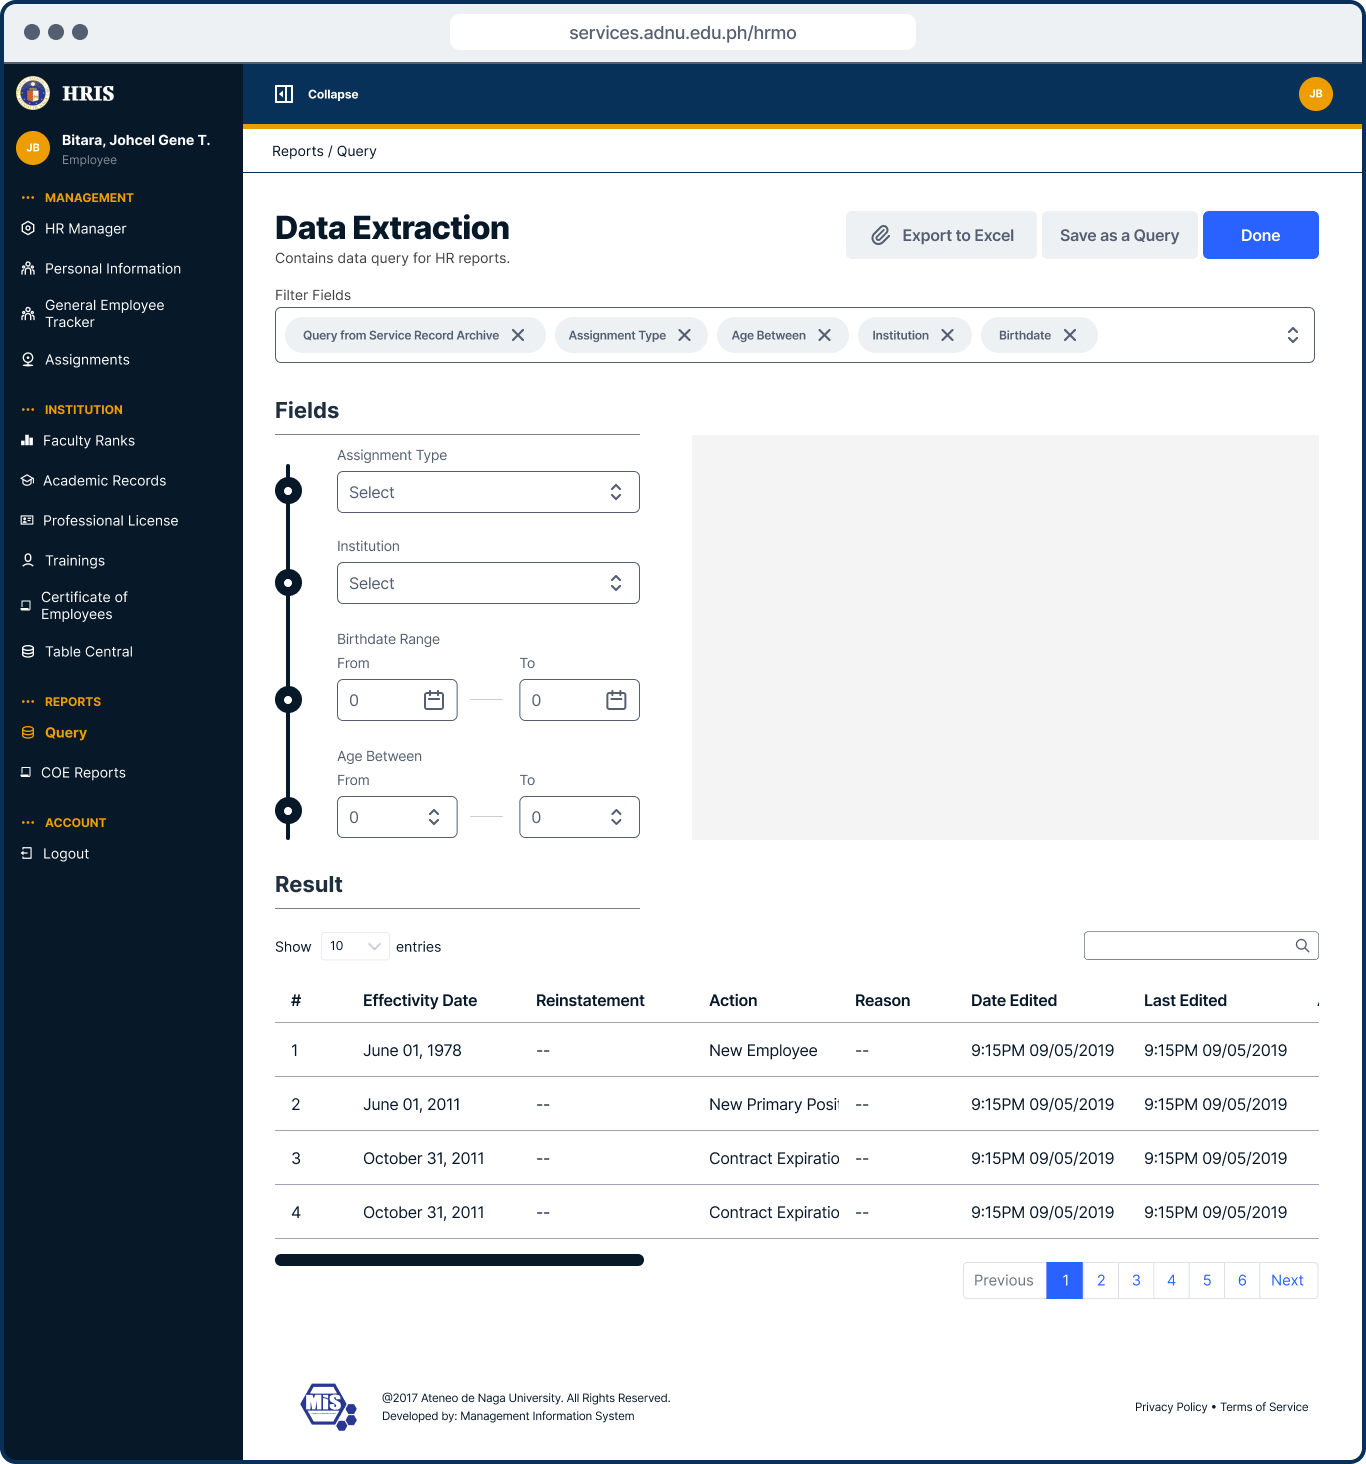
\includegraphics[width=1\linewidth]{figures/app/data-extraction.png}}
        \caption{Redesigned Data Extraction Page.}
        \label{fig:app-data-extraction}
    \end{figure}

    In this page, is the date extraction or query page for HR managers to extract reports. The interface is designed to facilitate efficient retrieval of HR data, likely offering options for customizable reports, data filtering, and exporting functionalities in Excel or CSV format.

    \begin{figure}[H]
        \centering
        \frame{\includegraphics[width=1\linewidth]{figures/app/chronos.png}}
        \caption{Redesigned Chronos Page.}
        \label{fig:app-chronos}
    \end{figure}

    The CHRONOS is designed as an interface for employee attendance in connection with DTR scanner devices to record employee attendance by scanning/tapping their ID cards. This record is then used to compute for the employee's tardiness, overtime, and absences in the figure \ref*{fig:app-attendance-emp}.
% %%%%%%%%%%%%%%%%%%%%%%%%%%%%%%%%%%%%%%%%%%%%%%%%%%%%%%%%%%%%%%%%%%%%%%%%%%%
\chapter{Results and Discussion}
%%%%%%%%%%%%%%%%%%%%%%%%%%%%%%%%%%%%%%%%%%%%%%%%%%%%%%%%%%%%%%%%%%%%%%%%%%%

Results and Discussion goes here...
% %%%%%%%%%%%%%%%%%%%%%%%%%%%%%%%%%%%%%%%%%%%%%%%%%%%%%%%%%%%%%%%%%%%%%%%%%%%
\chapter{Contributions and Recommendations}
%%%%%%%%%%%%%%%%%%%%%%%%%%%%%%%%%%%%%%%%%%%%%%%%%%%%%%%%%%%%%%%%%%%%%%%%%%%

Contributions and Recommendations goes here...
% %%%%%%%%%%%%%%%%%%%%%%%%%%%%%%%%%%%%%%%%%%%%%%%%%%%%%%%%%%%%%%%%%%%%%%%%%%%
\chapter{Conclusion}
%%%%%%%%%%%%%%%%%%%%%%%%%%%%%%%%%%%%%%%%%%%%%%%%%%%%%%%%%%%%%%%%%%%%%%%%%%%

Conclusion goes here... may also be used

\appendix
    \chapter{Interview Transcript}

\label{AppendixB}

To further understand the processes of the current HRIS along with specific details, the researchers sent a formal interview request letter on July 1, 2024. The document has undergo-ed reviews, approval, and endorsement of the SP Adviser/Dean/CITO/CSIO, as well as the CCS Chairperson, and given that the project is an MIS initiative, the approval of the MIS Director is requested.

On July 5, 2024, the researchers conducted a formal interview along with the System Administrator Specialist, HRMO -- Ms. Leanne Gemelly B. Briones. The interview lasted from 3:00PM to 4:00PM.

The interview covered various aspects of the current HRMO system and processes, starting from a general overview regarding HRIS to user experience, system limitations, data management, current requirements, and diagrams and documents. This allowed the researchers to better gain understanding of the processes and identify priorities within modules to create and disregard.

\begin{figure}[H]
    \centering
    \includegraphics[width=.78\linewidth]{figures/misc/minutes/interview-letter-request.jpg}
    \caption{Formal Interview Request.}
    \label{fig:interview-letter-request}
\end{figure}

\begin{figure}[H]
    \centering
    \includegraphics[width=1\linewidth]{figures/misc/minutes/interview-transcript-0001.jpg}
    \caption{Interview Transcript Page 1.}
    \label{fig:interview-transcript-0001}
\end{figure}

\begin{figure}[H]
    \centering
    \includegraphics[width=1\linewidth]{figures/misc/minutes/interview-transcript-0002.jpg}
    \caption{Interview Transcript Page 2}
    \label{fig:interview-transcript-0002}
\end{figure}

\begin{figure}[H]
    \centering
    \includegraphics[width=1\linewidth]{figures/misc/minutes/interview-transcript-0003.jpg}
    \caption{Interview Transcript Page 3}
    \label{fig:interview-transcript-0003}
\end{figure}

\begin{figure}[H]
    \centering
    \includegraphics[width=1\linewidth]{figures/misc/minutes/interview-transcript-0004.jpg}
    \caption{Interview Transcript Page 4}
    \label{fig:interview-transcript-0004}
\end{figure}
    % \chapter{Sample Reports}

Describe and discuss the details of sample reports here.

    % \chapter{Sample Input/Output}

Describe and discuss the details of sample I/O here.

    % \chapter{Code Listing}

\lstinputlisting{src/scs-greedy.cpp}

    % \chapter{User's Guide}




\nocite{*}
\bibliographystyle{siam}
{
\singlespace
\bibliography{references}
}

\begin{vita}

Johcel Gene T. Bitara is a BS Information Technology student of the Department of Computer Science at the Ateneo de Naga University.
\\
\\
Miguel Damien L. Garcera is a BS Information Technology student of the Department of Computer Science at the Ateneo de Naga University.
\\
\\
\end{vita}

\end{document}
